\documentclass[
  11pt,a4paper,twoside,openright,
  bibliography=totoc,listof=totoc,
  captions=tableheading,headings=normal,numbers=noenddot
]{scrbook}

\usepackage[T1]{fontenc}
\usepackage[utf8]{inputenc}
\usepackage{lmodern}
\usepackage[english]{babel}
\usepackage[autostyle,english=american]{csquotes}
\usepackage{microtype}
\usepackage[inner=3.0cm,outer=2.5cm,top=2.5cm,bottom=2.7cm]{geometry}
\usepackage{setspace}
\onehalfspacing
\emergencystretch=3em
\usepackage{graphicx}
\graphicspath{{figures/}}
\usepackage{array,booktabs,tabularx,tabulary,longtable,multirow,makecell,threeparttable}
\usepackage{xcolor}
\usepackage{tikz}
\usetikzlibrary{arrows.meta,positioning,fit,calc}
\usepackage{caption,subcaption}
\usepackage{enumitem}
\usepackage{amsmath,amssymb}
\usepackage{listings}
\usepackage[
  style=authoryear,backend=biber,maxcitenames=3,mincitenames=1,
  maxbibnames=99,giveninits=true,uniquename=init,uniquelist=false,
  doi=true,url=true,isbn=false,dashed=false,natbib=true
]{biblatex}
\addbibresource{references.bib}
\usepackage[hidelinks,pdfencoding=auto]{hyperref}
\usepackage{xurl}
\usepackage[nameinlink,capitalize,noabbrev]{cleveref}

\captionsetup{format=plain,labelfont={bf,small},font=small,skip=6pt,
  justification=RaggedRight,singlelinecheck=false}
\captionsetup[table]{position=top,skip=4pt}
\captionsetup[figure]{position=bottom,skip=6pt}
\setkomafont{disposition}{\rmfamily\bfseries}
\setkomafont{title}{\rmfamily\bfseries}

\newcommand{\MPR}{\textsc{mpr}}
\newcommand{\MI}{\textsc{mi}}
\newcommand{\kstar}{$k^{\ast}$}
\newcommand{\ie}{\textit{i.e.}}
\newcommand{\eg}{\textit{e.g.}}
\newcommand{\cf}{\textit{cf.}}

\title{Audited Semantic Propagation in LLM-Agent Societies\\
Persona Composition, Network Topology, and Climate Firestorms}
\author{[CANDIDATE NAME]}
\date{[SUBMISSION DATE]}

\begin{document}
\frontmatter

\begin{titlepage}
\centering
{\Large Technical University of Munich\par}
\vspace{0.4cm}
{\large [SCHOOL OR DEPARTMENT]\par}
\vspace{2.2cm}
{\huge\bfseries Audited Semantic Propagation in LLM-Agent Societies\par}
\vspace{0.4cm}
{\Large Persona Composition, Network Topology, and Climate Firestorms\par}
\vfill
{\Large Master's Thesis\par}
\vspace{1.2cm}
\begin{tabular}{@{}ll@{}}
Candidate: & [CANDIDATE NAME] \\
Student ID: & [MATRICULATION NUMBER] \\
Programme: & [DEGREE PROGRAMME] \\
First examiner: & [FIRST EXAMINER] \\
Supervisor: & [SUPERVISOR NAME] \\
Advisor: & [ADVISOR NAME, IF APPLICABLE] \\
Submission date: & [SUBMISSION DATE] \\
\end{tabular}
\vfill
{\small TUM-compatible KOMA-Script fallback. The named official template
\texttt{6aaeb12d2d2eaea03e67a80b} was unavailable at integration time.\par}
\end{titlepage}

\chapter*{Abstract}
\addcontentsline{toc}{chapter}{Abstract}
Online firestorms can connect scientific proposals with established
misinformation narratives. This thesis examines how factual content changes
when large language model (LLM) agents transmit climate and geoengineering
messages. It extends a prior auditor--node instrument with persona compositions,
eight generated topologies, and a separate 63-node complex network. Four
research questions address measurement, persona composition, topology, and
empirical anchoring.

The canonical Phase~2 campaign used \texttt{gpt-4o-mini}, eight hops, one run
per configuration, 288 configurations, and 1,728 article cells. It retained
292 cells with at most one scored event as hatched dead cascades. Continuous
and dual-discrete Misinformation Propagation Rate (MPR) remained separate.
Dual-discrete scores exceeded continuous scores on every topology aggregate,
which demonstrates instrument sensitivity rather than a common-scale increase.
Conspiracy-oriented personas and conspiracy-heavy mixes scored above scientific
personas and the conspiracy-free mix in both instruments. Topology conditioned
these contrasts, but no universal ranking emerged.

The D-net experiment applied the same protocol to a 63-node hashtag
co-occurrence graph. Conspiracy-only assignments exceeded mixed assignments on
both articles and instruments. Structural validation failed overall. The graph
was not a hydrated retweet cascade, empirical timing was unavailable, and
Debnath et al.\ provided no empirical Twitter MPR. The results therefore support
a traceable archived mechanism probe, not a causal account of human behaviour
or a validated digital twin. The selected runs also recorded 64,270 HTTP-error
responses; a zero-error-run sensitivity reversed the small continuous H--He
contrast but not the dual-discrete contrast.

\chapter*{Individual contribution and prior-work boundary}
\addcontentsline{toc}{chapter}{Individual contribution and prior-work boundary}
The auditor--node engine, MI, MPR, and the general-news linear-chain study are
co-authored prior work \parencite{maurya2025simulating}. The climate corpus,
Phase~2 campaign, Pfeffer operationalisation, composition analysis, and D-net
boundary test form the thesis research layer. \textbf{Unresolved placeholder:}
the candidate must insert the exact sentence-level division of code,
experimental design, analysis, and writing among all co-authors before
submission.

\chapter*{Declaration}
\addcontentsline{toc}{chapter}{Declaration}
\textbf{Official wording required.} Insert the current statutory declaration
from the responsible TUM examination office here. The official text, place,
date, signature fields, and any generative-AI disclosure were not available in
the source material and have not been invented.

\tableofcontents
\listoffigures
\listoftables

\chapter*{Abbreviations}
\addcontentsline{toc}{chapter}{Abbreviations}
\begin{description}[style=multiline,leftmargin=3.7cm]
  \item[D-net] Separate 63-node custom complex network.
  \item[DTFS] Digital Twin Fidelity Score.
  \item[H] Homogeneous persona assignment.
  \item[He] Heterogeneous persona assignment.
  \item[IFD] Information Fidelity and Distortion record.
  \item[LLM] Large language model.
  \item[MI] Misinformation Index.
  \item[MPR] Misinformation Propagation Rate.
  \item[T2c] Phase~2 continuous-instrument campaign.
  \item[T2d] Phase~2 dual campaign with a discrete headline.
  \item[\(k^{*}\)] First tick above MI 3 with no later observed recovery.
\end{description}

\mainmatter
% Draft chapter. Bibliography keys are placeholders pending integration with the
% thesis-wide .bib file. A source checklist appears at the end of this file.

\chapter{Introduction}
\label{chap:introduction}

\section{Problem and motivation}
\label{sec:introduction_problem}

Online misinformation changes as people repeat, reinterpret, and contest it.
This process matters when a scientific proposal becomes attached to an established conspiracy narrative.
Solar geoengineering provides such a case.
Public discussion of stratospheric aerosol intervention and Harvard's SCoPEx project has intersected with claims about chemtrails, weather control, and elite manipulation \parencite{debnath2023conspiracy}.
These claims can affect how citizens interpret research, institutions, and climate policy.
The relevant problem is therefore not only whether false content travels.
It is also how network structure and social identity shape factual change during transmission.

Online firestorm theory offers a social account of rapid, affective, and clustered communication.
Pfeffer, Zorbach, and Carley describe an online firestorm as a sudden volume of negative word of mouth directed at a person, company, or group \parencite{pfeffer2014firestorms}.
Their Outlook identifies seven interrelated factors: speed and volume, binary choices, network clusters, unrestrained information flow, lack of diversity, cross-media dynamics, and network-triggered decision processes.
The theory explains why particular communication environments can intensify collective reactions.
It does not specify a generative agent model or a quantitative tipping rule.

Geoengineering discourse supplies an empirical setting in which several of these mechanisms may matter.
Debnath and colleagues analysed 814,924 English-language tweets containing the geoengineering hashtag between 2009 and 2021 \parencite{debnath2023conspiracy}.
They identified a prominent chemtrails discourse alongside climate-action and environmental-concern themes.
They also documented temporal changes around solar-radiation-management projects and governance events.
Their study maps observed discourse at scale.
It does not provide controlled counterfactuals in which the same message enters different networks or identity compositions.

Agent simulation can provide such control, but it introduces a separate validity problem.
Classical cascade models represent diffusion through states or activation probabilities \parencite{kempe2003influence}.
They can isolate structural mechanisms, but they do not directly represent claim-level changes in natural language.
Large language model agents can transform text while retaining persona and interaction context.
Their outputs, however, reflect prompts, model behaviour, and scoring choices rather than observed human conduct.
Generative social simulations must therefore expose their assumptions and restrict claims to the evidence that their design supports \parencite{sargent2013verification}.

Maurya and colleagues provide the immediate technical basis for this thesis.
Their LASS workshop paper at ACM CIKM 2025 introduced an auditor--node framework for persona-conditioned rewrites on linear chains \parencite{maurya2025simulating}.
The framework scores factual degradation through a misinformation index (MI) and aggregates scores through a misinformation propagation rate (MPR).
That study used general-news domains, fixed chains of up to 30 rewrites, and a discrete question-answering auditor.
Its framework and published findings are prior work.
This thesis neither reintroduces those metrics nor reuses its crime and commercial results as new evidence.

\section{Research gap}
\label{sec:introduction_gap}

The three preceding research strands leave a specific methodological gap.
Pfeffer et al.\ provide a theory of firestorm conditions without a generative testbed.
Debnath et al.\ provide an observational account of geoengineering discourse without controlled interventions on network structure or identity composition.
Maurya et al.\ provide a generative misinformation instrument without a climate corpus, a graph-topology comparison, or an explicit mapping to firestorm theory.
The gap addressed here lies at their intersection.
It concerns how to design and audit a controlled climate-firestorm simulation without treating simulation output as observed social behaviour.

The proposal framed this intersection as six factors: valence, surprise, identity alignment, network clustering, information echo, and temporal acceleration.
Those labels are not Pfeffer et al.'s original seven-factor list.
This thesis treats them as a computational remapping.
It also records the parts that the simulation does not implement.
Cross-media dynamics has no media-broadcast layer.
Binary platform choices have no direct analogue because agents may forward, reinterpret, or drop a message.
Surprise remains a single-node drip seed, and the temporal horizon remains fixed.
The study therefore evaluates selected mechanisms rather than claiming to reproduce the complete firestorm theory.

Measurement creates a second gap inside the simulation.
The prior discrete auditor counts omitted and contradicted answers.
The present campaign also uses a continuous factual-recovery score.
These instruments share an approximate range but not a common measurement scale.
A difference between their outputs may reflect scoring design rather than a different social process.
The analysis must therefore keep discrete and continuous MI separate.

Empirical grounding creates a third constraint.
The public Debnath artefacts available to this study did not yield hydrated tweet text or conversation cascades.
The thesis consequently uses theory-faithful behavioural-profile reductions.
It also uses a 63-node hashtag co-occurrence graph as a structural fallback.
Neither object is an empirical user cluster or a retweet network.
This distinction prevents the simulation from being described as a digital twin of Twitter.

\section{Aim and analytical approach}
\label{sec:introduction_aim}

This thesis aims to develop and evaluate an exploratory artificial-society testbed for climate-misinformation propagation.
The testbed extends the prior auditor--node framework with climate and geoengineering seeds, Debnath-grounded behavioural profiles, and configurable network topologies.
It maps the firestorm theory to simulation controls, held conditions, and measured outcomes.
It then tests how identity composition, topology, and auditor design shape measured factual degradation.

The main campaign crosses eight graph topologies with two identity designs and two scoring modes.
The topologies are a linear chain, ring, Erdős--Rényi graph, small-world graph, scale-free graph, echo chamber, polarised graph, and hierarchy.
The homogeneous arm assigns one of 12 behavioural profiles to all eight nodes.
The heterogeneous arm assigns one of six eight-profile mixtures.
Each configuration processes six climate or geoengineering articles over eight ticks.
The resulting design contains 1,728 article-level cells.
All cells use \texttt{gpt-4o-mini}, one graph seed, and one stochastic run.

The analysis reports MI and mean node MPR within each scoring mode.
It defines \(k^{*}\) as the first tick at which mean MI exceeds 3 and remains above 3 for every later observed tick.
This quantity is a right-censored simulator clock.
It is not an estimate of ignition time on social media.
The analysis also retains 292 cells with at most one scored event as hatched dead cascades.
It excludes those cells from live-cell means but does not recode them as zero.

A separate D-net analysis places the same agents on the 63-node hashtag graph.
This analysis compares simulated cascade shape with the documented fallback structure.
It also compares homogeneous conspiracy profiles with a mixed profile assignment on the same edge set.
The comparison concerns graph structure and simulated auditor scores.
Debnath et al.\ report no empirical MI or MPR against which those scores could be validated.

\section{Research questions}
\label{sec:introduction_rqs}

The study addresses four research questions.
Each question follows from a design choice that the available evidence can evaluate.

\begin{enumerate}
    \item[\textbf{RQ1}] \textbf{Holding identity arm and topology labels fixed, how do the continuous and dual-discrete auditor instruments change estimated misinformation severity, \(k^{*}\) occurrence, and topology ordering?}

    RQ1 treats scoring mode as a measurement question.
    It compares modes without averaging their values or interpreting their gap as a third misinformation measure.

    \item[\textbf{RQ2}] \textbf{Within one scoring mode, does explicit conspiracy composition explain misinformation severity and \(k^{*}\) occurrence more consistently than the coarse homogeneous or heterogeneous label?}

    RQ2 compares persona families and named mixtures.
    It treats composition as substantive and H or He as an assignment description.

    \item[\textbf{RQ3}] \textbf{How does topology condition the same-mode relationship between persona composition, live-cell MI, and irreversible \(k^{*}\) within the eight-tick horizon?}

    RQ3 compares the eight generated topologies.
    It reports dead-cell rates with live-cell means because cascade survival changes the observed population.

    \item[\textbf{RQ4}] \textbf{What can the 63-node hashtag-based D-net comparison establish about structural similarity and identity-conditioned factual degradation, and where does that comparison fail?}

    RQ4 separates empirical graph properties from simulated content scores.
    It tests a documented fallback rather than claiming reconstruction of Debnath et al.'s tweet cascades.
\end{enumerate}

These questions support descriptive comparisons.
They do not support population estimates or causal effects.
The single stochastic run also precludes confirmatory inference about topology, identity, or scoring mode.

\section{Contributions}
\label{sec:introduction_contributions}

This thesis makes four bounded contributions.

\begin{enumerate}
    \item It provides an explicit mapping from Pfeffer et al.'s seven firestorm factors to the simulation's varied, held, measured, and absent elements.
    The mapping corrects the proposal's six-factor shorthand and retains cross-media dynamics as an unimplemented boundary.

    \item It constructs a documented climate and geoengineering simulation layer for the prior auditor--node framework.
    This layer contains six campaign articles, 12 homogeneous behavioural profiles, six heterogeneous mixtures, eight topologies, and reproducible configuration files.
    The profiles reduce themes reported by Debnath et al.; they are not clusters estimated from 814,924 tweets.

    \item It evaluates identity composition and network topology under two distinct factual-degradation instruments.
    The analysis preserves dead cascades, separates continuous from discrete scores, and distinguishes persona composition from the broad homogeneous--heterogeneous contrast.

    \item It links a 63-node hashtag co-occurrence structure to a custom simulation graph and audits the limits of that comparison.
    This analysis reports structural mismatch as well as similarity.
    It does not equate auditor MI with Twitter behaviour.
\end{enumerate}

These contributions concern operationalisation, experimental design, and transparent measurement.
They do not include the original auditor--node architecture, MI, MPR, or the published linear-chain findings.
They also do not establish a validated model of public response to geoengineering.

\section{Scope and limitations}
\label{sec:introduction_scope}

The empirical scope is deliberately narrow.
The campaign uses six authored or curated climate articles and a finite set of prompt-based behavioural profiles.
It runs eight-node graphs for eight ticks with one model and one graph seed.
The design changes text through LLM role-play.
It does not model stable human belief, individual psychology, or platform recommendation systems.

The data scope is narrower than the proposal anticipated.
The study did not hydrate the 814,924 tweet identifiers.
It did not estimate HDBSCAN profiles, reconstruct conversation trees, or reproduce Debnath et al.'s temporal series.
The hashtag graph records co-occurrence structure, not retweet transmission.
The simulation clock cannot be converted into minutes, days, or empirical hop distance.

The inferential scope follows these design limits.
The results describe one stochastic campaign.
They do not warrant significance claims, robust rankings, or general laws about homogeneous and heterogeneous groups.
The two auditors remain model-based measurements.
Their disagreement is evidence about the instrument, not an independent factual ground truth.
The \(k^{*}\) measure is conditional on the eight-tick observation window.
A value of ``none'' means that no irreversible crossing appeared within that window.

\section{Thesis roadmap}
\label{sec:introduction_roadmap}

Chapter~\ref{chap:related_work} develops the theoretical and empirical background.
It covers online firestorms, climate and geoengineering discourse, diffusion models, LLM-agent simulation, and automated factuality assessment.
Chapter~\ref{chap:theory} maps Pfeffer et al.'s seven factors to the thesis design.
Chapter~\ref{chap:methods} separates the inherited system from the climate-specific design and documents the articles, behavioural profiles, and hashtag graph.
Chapter~\ref{chap:methods} specifies the factorial campaign, both auditor modes, dead-cell rule, and \(k^{*}\).
Chapter~\ref{chap:results} answers RQ2 and RQ3 across the 1,728-cell campaign.
It then answers RQ4 through the D-net comparison.
Chapter~\ref{chap:discussion} interprets the findings against Pfeffer, Debnath, and the prior linear-chain study.
Chapter~\ref{chap:limitations} addresses validity, ethics, and reproducibility.
Chapter~\ref{chap:conclusion} answers the research questions and states the conditions required for stronger claims.

The thesis therefore proceeds from theory to operationalisation, from operationalisation to measurement, and from measurement to bounded interpretation.
Its central claim is methodological.
An LLM society can expose how climate-misinformation results depend on identity, topology, and the scoring instrument, but this campaign cannot stand in for the public it simulates.

% ---------------------------------------------------------------------------
% COMPANION SOURCE LIST FOR THIS DRAFT
% Add or verify these records in the thesis-wide bibliography before compiling.
%
% pfeffer2014firestorms
%   Pfeffer, J.; Zorbach, T.; Carley, K. M. (2014).
%   Understanding Online Firestorms: Negative Word-of-Mouth Dynamics in
%   Social Media Networks. Journal of Marketing Communications, 20(1--2),
%   117--128. DOI: 10.1080/13527266.2013.797778.
%   Supports: firestorm definition and original seven-factor Outlook.
%
% debnath2023conspiracy
%   Debnath, R. et al. (2023). Conspiracy Spillovers and Geoengineering.
%   iScience, 26(3), 106166. DOI: 10.1016/j.isci.2023.106166.
%   Supports: 814,924-tweet observational corpus, discourse themes, and
%   geoengineering context. It does not provide empirical MI or MPR.
%
% maurya2025simulating
%   Maurya, R. G. et al. (2025). Simulating Misinformation Propagation in
%   Social Networks using Large Language Models. 1st Workshop on LLM Agents
%   for Social Simulation (LASS), ACM CIKM 2025. arXiv:2511.10384.
%   Supports: prior auditor--node framework, MI/MPR, severity bands, and
%   30-hop linear-chain study. Cite as workshop work, not CIKM main track.
%
% kempe2003influence
%   Kempe, D.; Kleinberg, J.; Tardos, E. (2003). Maximizing the Spread of
%   Influence through a Social Network. KDD '03, 137--146.
%   DOI: 10.1145/956750.956769.
%   Supports: activation-based cascade-model contrast.
%
% tornberg2024validation
%   Törnberg, P. et al. (2024). Validation is the central challenge for
%   generative social simulation. Journal of Computational Social Science.
%   Verify final author list, volume, pages, and DOI before submission.
%   Supports: validation limits of generative social simulation.
%
% Internal evidence used for design statements, not bibliography entries:
%   thesisExperiment/PHASE2_PLAN.md
%   thesisExperiment/LOG.md
%   thesisExperiment/results_phase2/summary.json
%   thesisExperiment/analysis_phase2/SUMMARY.md
%   thesisExperiment/analysis_full/COMPARISONS.md
%   thesisExperiment/analysis_full/PFEFFER_DEBNATH_VS_SIM.md
%   thesisExperiment/analysis_phase2/PFEFFER_FIRESTORM.md
%   thesisExperiment/discovery/01_literature/_extract/proposal_pfeffer_v5.txt
%   thesisExperiment/discovery/01_literature/do_not_reprint.md
% ---------------------------------------------------------------------------

\chapter{Literature Review}
\label{chap:related_work}

This chapter locates the thesis at the intersection of misinformation diffusion,
online-firestorm theory, geoengineering discourse, network science, and
large-language-model (LLM) agent simulation.  The distinction between these
literatures matters.  A model may reproduce the reach of a cascade without
representing how its claims change, while fluent agent output may look socially
plausible without constituting a valid model of people.  The review therefore
connects substantive theory to the thesis's observables and closes by stating
the specific gap addressed by the experiments.

\section{Misinformation as diffusion and semantic transformation}
\label{sec:lit-misinformation}

Misinformation is not a single technical object.  The term can refer to false
content, an actor's belief, an exposure, a sharing decision, or a population-level
diffusion pattern.  \textcite{lazer2018science} consequently call for research
that joins individual cognition, institutions, and platform structure rather
than treating falsity as a classification problem alone.  Large-scale
observational evidence confirms that diffusion is socially structured:
\textcite{vosoughi2018false} found that false news on Twitter travelled farther,
faster, deeper, and more broadly than true news in their data.  Novelty and
emotional response helped distinguish false from true cascades, while automated
accounts accelerated both.  These findings motivate models with content and
agent state, but they do not imply that every simulated cascade should reproduce
the same ordering.

Classical diffusion models provide useful null formalisms.  In the independent
cascade model, an activated node receives one probabilistic opportunity to
activate each neighbour \parencite{kempe2003influence}.  Related compartmental
and threshold models reduce the state of a node to susceptible, active, adopted,
or an opinion scalar.  Their abstraction is an advantage for identifying
conditions for reach or consensus, but an edge transmits a state rather than
rewriting a proposition.  This thesis instead studies a transmission in which
the text itself can lose, invert, or acquire claims.  The distinction is between
\emph{whether} something propagates and \emph{what it becomes while propagating}.

Empirical cascade size is also not synonymous with virality.
\textcite{goel2016virality} show that similarly popular diffusion events range
from broadcast-like stars to multigenerational chains and define structural
virality from pairwise distances in a diffusion tree.  A scale-free contagion
model did not recover the full empirical diversity they observed.  This is a
warning against explaining an outcome from a topology label alone.  In the
present study, event count, semantic degradation, and time to a severity
threshold are therefore conceptually separate outcomes.

\section{Online firestorms: theory and operationalisation}
\label{sec:lit-firestorms}

\textcite{pfeffer2014firestorms} define an online firestorm as a sudden discharge
of large quantities of negative word-of-mouth and complaint behaviour directed
at a person, organisation, or group.  Their contribution is a qualitative
synthesis of the mechanisms that make rapid, affective outrage possible.  The
paper's outlook identifies \emph{seven} interrelated factors: speed and volume
of communication, binary choices, network clusters, unrestrained information
flow, lack of diversity, cross-media dynamics, and network-triggered decision
processes.  It does not present an agent-based generative model, a semantic
misinformation scale, or a tipping-time estimator.

This point prevents a common attribution error.  The six simulation dimensions
used in this thesis---valence, surprise, identity alignment, network clustering,
information echo, and temporal acceleration---are a \emph{computational
remapping}, not Pfeffer et al.'s original list.  Valence represents the affective
character of firestorm messages.  Identity alignment and information echo
approximate lack of diversity and clustered reinforcement.  Network clustering
maps directly to local structure, while surprise and temporal acceleration
separate seeding shocks from the speed of subsequent exchange.  Cross-media
dynamics has no equivalent in the present single-platform society and is a
boundary condition.  Nor does the simulator reproduce the original paper's
binary platform affordances in a literal way.  The remapping is thus an
operational hypothesis to be assessed, not a claim that all seven mechanisms
have been implemented.

Later work has moved toward measuring observed firestorms.
\textcite{nuortimo2020scale} propose a three-level scale based on a media-analytics
case, and \textcite{nuortimo2025scale} develop dimensions of firestorm width,
intensity, and peak duration with AI-assisted validation.  These studies make
event severity more explicit, but remain different from a claim-level instrument
applied during a controlled generative cascade.  The literature leaves open how
a theory of rapid collective outrage should be connected to the semantic
mutation of scientific information.

\section{Geoengineering discourse as the substantive case}
\label{sec:lit-geoengineering}

Solar geoengineering is an unusually demanding case for studying that
connection.  Discussion combines scientific uncertainty, climate politics,
governance, distrust, and established conspiracy narratives.  It therefore
cannot be represented adequately as generic ``fake news.''  The principal
empirical grounding is \textcite{debnath2023conspiracy}, who analysed 814,924
English-language tweets containing \texttt{\#geoengineering} from 2009 to 2021.
Using natural-language processing, toxicity analysis, word embeddings, and
network analysis, they show that the false chemtrails narrative substantially
shaped geoengineering discussion.  Conspiracies spilled into debates in the
United Kingdom, United States, India, and Sweden and connected with broader
political themes.  Positive emotions tended to increase following governance
events, whereas negative and neutral emotions increased around project and
experiment announcements; toxicity widened anti-solar-radiation-management
spillovers.

Debnath et al. establish an observational association, not a causal diffusion
model or an LLM-agent society.  Their corpus is nevertheless valuable for
defining plausible discourse tendencies and seed events.  This thesis derives
reduced belief profiles for conspiracy, climate-action, and environmental-concern
positions from that account.  These profiles are \emph{theory-grounded types};
they are not user clusters or fitted population proportions.  The public data
deposit contains tweet identifiers \parencite{debnath2023dataset}.  The thesis
did not hydrate and recluster the 814,924 tweets and therefore does not claim to
replicate Debnath et al.'s analysis, infer their social graph, or construct a
Twitter digital twin.

This separation supports a defensible use of the case.  The observational study
supplies the empirical phenomenon---chemtrails-related spillover, affect, and
toxicity---while the simulation supplies counterfactual control over seeds,
identity composition, and network structure.  Agreement between the two would
be evidence of external plausibility, not proof that the simulated agents are
the users in Debnath et al.'s data.

\section{Network topology, homophily, and echo}
\label{sec:lit-topology}

Topology changes who can expose whom and how many independent or reinforcing
paths connect groups.  Erd\H{o}s--R\'enyi graphs provide a random-graph reference
\parencite{erdos1960evolution}; Watts--Strogatz networks combine local clustering
with short paths \parencite{watts1998collective}; and preferential attachment
generates heavy-tailed degree distributions and hubs
\parencite{barabasi1999emergence}.  These models are not interchangeable proxies
for real social media.  They are controlled structural hypotheses whose degree
distribution, clustering, path length, and seed position must be reported.

The content being transmitted also changes which topology should facilitate
diffusion.  \textcite{centola2007complex} distinguish simple contagion, for which
one contact may suffice, from complex contagion requiring reinforcement from
multiple neighbours.  Long weak ties can accelerate the former but fail to
provide sufficiently wide bridges for the latter.  Firestorm participation and
conspiracy reinterpretation may involve social affirmation and are therefore
not safely assumed to behave like infection over a single edge.

Agent composition and topology are joined by homophily.  Similarity structures
social ties and thereby the information, attitudes, and interactions available
to people \parencite{mcpherson2001homophily}.  Empirically, selective exposure and
homogeneous interaction can support polarised information communities:
\textcite{delvicario2016echo} relate emotional contagion and group polarisation
in Facebook communities, while \textcite{tornberg2018echo} models viral
misinformation as a complex contagion.  A high-level ``echo chamber'' label,
however, is not a measurement.  This thesis therefore distinguishes treatment
variables (network generator and persona assignment) from observables such as
edge homophily and community separation.  Modularity compares within-group
edge density with a degree-preserving null expectation
\parencite{newman2006modularity}; it indicates structural segregation, not the
truth or extremity of group content.

\section{Homogeneous and heterogeneous agent populations}
\label{sec:lit-heterogeneity}

Homogeneous-agent models isolate a response rule and simplify attribution, but
they can turn an imposed persona into a population-wide mechanism.
Heterogeneous populations permit cross-cutting exposure, specialist roles, and
different propensities to reinterpret or resist a message.  At the same time,
heterogeneity is not intrinsically realistic.  Results depend on which types are
included, their prevalence, their network positions, and whether prompts create
genuine behavioural variation or merely labels.

The immediate methodological predecessor is the auditor--node system of
\textcite{maurya2025simulating}, presented at the LASS workshop at ACM CIKM
2025.  It compares persona-homogeneous and persona-heterogeneous linear rewrite
chains and introduces the discrete Misinformation Index (MI) and branch-level
Misinformation Propagation Rate (MPR).  Those general-news linear-chain findings
are \emph{prior work}, not results of this thesis.  The present work retains the
auditor--node idea but changes the empirical object to geoengineering discourse,
uses Debnath-grounded profiles, and introduces non-chain network treatments.

The broader literature demonstrates both the promise and the unresolved status
of LLM societies.  Social Simulacra populates prototypes of online communities
\parencite{park2022simulacra}, while Generative Agents combines memory,
reflection, and planning to create believable local interactions
\parencite{park2023generative}.  S$^3$ simulates information, attitude, and
emotion propagation against social-network data \parencite{gao2023s3}.  OASIS
adds platform actions, recommendation mechanisms, dynamic networks, and very
large populations \parencite{yang2024oasis}; AgentSociety similarly prioritises
large-scale social environments \parencite{piao2025agentsociety}.  These systems
expand scale and behavioural surface area, but scale does not by itself validate
an agent as a model of a person.

Most directly, \textcite{li2026diffusion} condition LLM-agent forwarding on
psychological traits and compare diffusion under different network structures,
including an empirical Higgs community.  Their topology-sensitive forwarding
study is close to this thesis, but the focal state remains sharing and diffusion
rather than audited claim-by-claim mutation in geoengineering text.  The
literatures are complementary: one asks whether an item is forwarded; this
thesis asks how the item's factual content changes as a function of identity
mix and topology.

Persona conditioning also creates a validity problem.  Language models can
reproduce some subgroup response patterns when conditioned on demographic
backstories \parencite{argyle2023one}, and they can recover qualitative patterns
from selected economic experiments \parencite{horton2023silicus}.  Such results
support LLMs as inexpensive theory probes, not synthetic replacements for human
participants.  Training-data contamination, prompt sensitivity, stochasticity,
stereotype amplification, limited within-group variance, and obedience to
experimenter instructions all threaten behavioural interpretation.  In this
thesis, ``homogeneous'' and ``heterogeneous'' consequently describe prompt
conditions in a computational experiment.  They do not denote representative
human populations.

\section{Measurement validity: discrete and continuous instruments}
\label{sec:lit-validity}

The thesis's central dependent variable is produced by an instrument, not
observed directly.  Construct validity concerns whether evidence supports the
interpretation and use of a score.  It cannot be established by naming a
quantity ``misinformation.''  \textcite{cronbach1955construct} require a measure
to sit in a nomological network connecting a construct to observable
consequences, and \textcite{messick1995validity} treats validity as an integrated
argument about score meaning, generalisation, external relations, and
consequences.  For MI, relevant evidence would include item coverage, human
agreement, expected relations with known distortions, stability across judges,
and sensitivity to irrelevant wording.

QA-based factuality evaluation supplies a methodological warrant.
\textcite{fabbri2022qafacteval} show that question answering can assess factual
consistency in summarisation more directly than lexical overlap.  LLM judges can
also agree substantially with human preferences, but exhibit position,
verbosity, and self-enhancement biases \parencite{zheng2023judge}.  Neither result
validates this thesis's exact instrument: fixed binary questions about
geoengineering, answered by an LLM judge, are a different construct and use
case.

The distinction between discrete and continuous scoring must therefore remain
visible.  In discrete MI, each item is classified as recovered, missing, or
contradicted and the item outcomes are aggregated into a bounded score.
This format is inspectable and corresponds to explicit propositions, but it
collapses uncertainty and treats all items as equally diagnostic.  A continuous
instrument can retain graded evidence or confidence and may detect smaller
changes, but its numeric precision is not automatically substantive precision.
It requires calibration and a defensible interpretation of distances between
scores.

The statistical literature cautions that converting a genuinely continuous
quantity into categories discards information, reduces power, and creates
artificial discontinuities around a cut point
\parencite{maccallum2002dichotomization,altman2006cost}.  That warning applies to
the thesis's severity bands: the boundary at MI${}>3$ is an operational decision
inherited from prior work, not a psychometrically established natural kind.
Conversely, the warning does not prove that a continuous LLM score is valid.
Discrete and continuous MPR are different instruments; they should not be pooled
or treated as interchangeable observations merely because both have numeric
output.

Shared generator and judge families add common-method dependence.  A fluent
rewrite may be rewarded because it resembles the judge's preferred formulation,
and a failed parse can masquerade as low misinformation if the implementation
fails open.  Credible validation therefore requires frozen test cases,
fail-closed parsing, deterministic judging where possible, manual inspection,
human coding of a sample, and agreement reported at the decision boundary used
for the substantive claim.  Until such evidence exists, MI and MPR are best
described as \emph{simulation audit scores}, not validated measures of human
misinformation belief.

\section{Validation of generative social simulation}
\label{sec:lit-simulation-validation}

Verification asks whether the program implements the intended model; validation
asks whether the model is adequate for its intended purpose.
\textcite{sargent2013verification} separates data validity, conceptual-model
validity, computerised-model verification, and operational validity.  For
agent-based social simulation, \textcite{richiardi2006protocol} further stress
transparent model description, sensitivity analysis, replication, and a
validation test matched to the claim.  \textcite{windrum2007validation} show that
empirical validation can involve several strategies and that no single fitted
trajectory settles model adequacy.

Applied here, validation has at least four levels.  First, software checks must
establish that topology, persona assignment, intervention timing, and auditor
aggregation behave as specified.  Second, internal validation asks whether
changing a theoretically relevant input produces stable, interpretable changes
rather than parser artefacts or dead cascades.  Third, output validation compares
patterns with held-out empirical regularities, such as plausible cascade
structure or Debnath's discourse themes.  Fourth, measurement validation asks
whether humans and independent instruments support the MI interpretation.
Face-plausible agent prose is evidence for none of these levels by itself.

The intended use defines the attainable claim.  A small, replicated, audited
model may function as a mechanism probe: it can test whether a proposed
combination of topology and identity is sufficient to produce a pattern under
specified prompts.  Without calibrated agent distributions and reconstructed
empirical cascades, it cannot estimate the prevalence or causal effect of that
mechanism among Twitter users.  Failed or near-empty cascades are execution or
design outcomes to diagnose, not evidence that a topology prevents
misinformation.  Stochastic LLM output also requires multiple seeds or models
before a directional contrast can be considered stable.

\section{Synthesis and research gap}
\label{sec:lit-gap}

The literature leaves a precise intersection underdeveloped.  Firestorm theory
identifies structural conditions for rapid, affective outrage but does not
provide a generative, claim-level model \parencite{pfeffer2014firestorms}.
Network diffusion research explains activation, reinforcement, and cascade
shape but usually treats content as a binary or fixed state
\parencite{kempe2003influence,centola2007complex}.  Debnath et al. provide a
large observational map of geoengineering conspiracy spillovers but not
controlled counterfactual societies \parencite{debnath2023conspiracy}.  LLM
societies generate heterogeneous behaviour at increasing scale, yet their
misinformation evaluations commonly emphasise sharing, aggregate plausibility,
or believability rather than a validated trajectory of proposition-level change.
Finally, the prior auditor--node study supplies MI/MPR and homogeneous versus
heterogeneous chains, but not a geoengineering-grounded network experiment
\parencite{maurya2025simulating}.

The gap filled by this thesis is therefore \emph{not} a new general-purpose agent
architecture and not a replication of an 814,924-tweet study.  It is a
theory-mapped, auditable test of how network topology and Debnath-grounded
identity composition jointly condition semantic misinformation trajectories in
geoengineering discourse.  It connects (i) an explicit seven-to-six Pfeffer
operationalisation, (ii) controlled homogeneous and heterogeneous LLM-agent
societies, and (iii) discrete and continuous claim-recovery instruments whose
validity limits remain explicit.  The empirical contribution is the resulting
climate-domain comparison and its validation evidence; the methodological
contribution is a separation of transmission, semantic mutation, firestorm
timing, and instrument choice.  This design addresses a question not answered
by any one parent literature: under fixed scientific seeds, are apparent
firestorm thresholds robust to who occupies the network, how those agents are
connected, and how factual degradation is measured?

\chapter{Theoretical Framework and Operationalisation}
\label{chap:theory}

\section{Conceptual framework}
\label{sec:theory}

\subsection{Purpose and analytical levels}

This thesis explains how factual content changes while it moves through a synthetic social network.
The explanation distinguishes three levels: persona composition determines which agents transform a message, topology determines potential exposure, and propagation links agent transformations and exposure over time.
The resulting texts are then scored with an explicit measurement instrument.

This sequence separates mechanism from measurement.
The simulated mechanism produces texts, actions, and exposure paths.
The auditor converts those texts into misinformation scores.
The scores are observations of the simulation.
They are not the mechanism itself.

The framework also separates misinformation from a firestorm.
Misinformation concerns departure from factual source claims.
An online firestorm concerns a rapid and large discharge of negative word-of-mouth \parencite{pfeffer2014firestorms}.
The two phenomena may coincide.
They need not coincide.
Accurate criticism can form a firestorm.
Severe misinformation can also diffuse slowly and quietly.
Therefore, Misinformation Index (MI) and Misinformation Propagation Rate (MPR) do not by themselves identify a firestorm.

Three kinds of statement follow from this distinction.
\emph{Theory} states a proposed relation among composition, topology, exposure, and content change.
\emph{Operationalisation} states how the relation is represented in the simulation.
\emph{Evidence} states what an observed source or experiment can support.
The distinction is maintained throughout this chapter.

\subsection{The integrated generative argument}
\label{subsec:integrated-causal-argument}

Let \(G=(V,E,W)\) be a directed network.
The node set \(V\) contains synthetic agents.
The edge set \(E\) defines possible transmissions.
The weights \(W\) represent relational conditions such as trust.
Each node \(i\) receives a persona \(p_i\).
The complete assignment is denoted by \(\boldsymbol{p}=(p_1,\ldots,p_{|V|})\).

Let \(X_e\) be the text carried by propagation event \(e\).
When node \(i\) processes the event at time \(t\), it applies a persona-conditioned transformation:
\begin{equation}
X_{e'} = T_{p_i}\!\left(X_e,\,H_i(t),\,R_i(t)\right).
\label{eq:persona-transform}
\end{equation}
Here, \(H_i(t)\) is the information available to the agent.
\(R_i(t)\) denotes local relational conditions.
The output may be forwarded, reinterpreted, or dropped.
Thus, propagation is a sequence of selective text transformations.
It is not the movement of a fixed information token.

The theoretical object is the joint process
\begin{equation}
\mathcal{Y}
=
F\!\left(
\boldsymbol{p},
G,
S,
A,
\mathcal{T},
\varepsilon
\right),
\label{eq:joint-process}
\end{equation}
where \(S\) is the seed message.
\(A\) is the action rule.
\(\mathcal{T}\) is the exposure schedule.
\(\varepsilon\) collects stochastic and model-specific variation.
\(\mathcal{Y}\) contains generated texts, transmissions, and cascade structure.
An auditor \(J\) then maps the generated texts to observed scores:
\begin{equation}
\widehat{\mathcal{M}} = J(\mathcal{Y};Q,G_Q,\theta_J).
\label{eq:measurement-map}
\end{equation}
The question set \(Q\), gold answers \(G_Q\), and auditor specification \(\theta_J\) are part of the measurement model.
They are not neutral bookkeeping choices.

The framework therefore has a clear order.
Composition and topology shape exposure.
Exposure selects which persona transformations occur.
Repeated transformations produce factual retention or drift.
The auditor then measures that drift.
Pfeffer's firestorm theory interprets the broader communication conditions.
Debnath's belief profiles ground the identities and issue domain.

\subsection{Persona composition as a transformation mechanism}
\label{subsec:persona-composition}

\paragraph{Theory.}
A persona is a structured prior over attention, interpretation, and expression.
It makes some source claims salient.
It makes other claims easy to omit or recode.
Repeated use of the same prior can compound a stable distortion.
Mixed priors can interrupt that process.
They can also introduce new distortions.
Heterogeneity is therefore not intrinsically corrective.

Composition has at least three dimensions.
The first is the share of each persona family.
The second is the diversity of those families.
The third is their placement in the graph.
Two societies can have the same shares but different outcomes.
One may place a conspiracy persona at a hub.
The other may place the same persona at the periphery.
The label ``heterogeneous'' does not capture this difference.

Results from the prior auditor--node preprint illustrate this dependence on composition and order.
In homogeneous 30-node branches, identity- and ideology-laden personas often accelerated drift.
Expert and neutral personas often stabilized factual content \parencite{maurya2025simulating}.
Yet the controlled-random heterogeneous branches reached the high-loss band
(\(\mathrm{MI}>3\)) in about \(85\%\) of branch--domain pairs.
The prior study therefore does not establish a general ``diversity buffers misinformation'' law.
It shows that persona effects depend on order, content, and repeated interaction.

\paragraph{Operationalisation.}
The thesis assigns persona identifiers and prompts to nodes.
Homogeneous conditions repeat a focal identity.
Heterogeneous conditions combine several identities.
The relevant treatment is the complete assignment \(\boldsymbol{p}\), not the H/He label alone.
Composition should therefore be reported as persona-family shares and node positions.
Results should also be conditioned on persona family.
A lower network mean may otherwise reflect fewer conspiracy seats rather than corrective interaction.

\paragraph{Evidence.}
The prior arXiv preprint provides simulation evidence for persona-conditioned drift on linear branches.
It does not provide human behavioural validation.
It also does not provide evidence about complex-network placement.
The present experiments can provide evidence about synthetic agents under fixed prompts and models.
They cannot establish that real users with similar labels would behave identically.

\subsection{Topology as an exposure mechanism}
\label{subsec:topology-exposure}

\paragraph{Theory.}
Topology affects factual content indirectly by determining which agents can receive and transform a message.
Degree controls how many transmissions can follow an event.
Path length controls how many sequential transformations can occur.
Clustering creates repeated exposure from connected neighbours.
Community structure concentrates exposure within groups.
Bridges permit a frame to cross between groups.
Hubs place selected agents in high-leverage positions.

Topology and composition are therefore non-separable.
A clustered graph does not create an identity echo unless identities align with its clusters.
A homogeneous graph produces perfect identity agreement by construction.
That agreement is not evidence of an emergent echo chamber.
Likewise, a scale-free graph is primarily a hub contrast.
It is not automatically a clustering contrast.

\paragraph{Operationalisation.}
The topology generator defines \(E\) and initial edge conditions.
Persona assignment then defines the relation between social position and identity.
The design includes chains, rings, random graphs, small-world graphs, scale-free graphs, echo chambers, polarised graphs, and hierarchical graphs.
Each topology represents a distinct exposure opportunity structure.
No generator is treated as a complete model of a platform.

The linear chain is the direct link to the prior arXiv preprint.
The small-world graph is the clearest named operationalisation of local clustering \parencite{watts1998collective}.
The scale-free graph represents unequal connectivity and hub exposure \parencite{barabasi1999emergence}.
The random graph provides a stochastic baseline \parencite{erdos1960evolution}.
The echo and polarised graphs encode pre-existing segregation.
They do not demonstrate that segregation emerged during the run.
The hierarchical graph represents asymmetric transmission.
It does not operationalise legacy-media feedback.

\paragraph{Evidence.}
Differences between topology cells are evidence about the implemented generators.
They are not evidence about all networks in the same named class.
One archived realisation per cell does not identify a topology-wide effect.
Dead cascades also carry information about reachability.
They must not be recoded as zero misinformation.

\subsection{Propagation as a coupled selection process}
\label{subsec:propagation}

\paragraph{Theory.}
Propagation determines which potential transformations become realized.
At each event, an agent may forward, reinterpret, or drop a message.
Forwarding preserves more of the received text.
Reinterpretation invokes another persona-conditioned rewrite.
Dropping ends that path.
The observed cascade is therefore selected by both network access and agent action.

This creates two distinct margins.
The extensive margin concerns whether content reaches another node.
The intensive margin concerns how much the content changes when it is processed.
A topology can increase reach without increasing factual drift per rewrite.
A persona can increase drift while reducing onward transmission.
These mechanisms should not be collapsed into one mean.

Repeated exposure adds a further mechanism.
Several neighbours may deliver related frames to the same node.
The node can then receive social confirmation as well as content.
Pfeffer describes this local echo as a consequence of network clusters \parencite{pfeffer2014firestorms}.
In the simulation, however, repeated receipt is an implemented exposure pattern.
It is not direct evidence of human persuasion.

\paragraph{Operationalisation.}
The simulator records event time, hop count, sender, receiver, action, and rewritten text.
Ticks and hops answer different questions.
A tick is a simulation update.
A hop is a position along a transmission path.
Neither is a unit of wall-clock time.
The eight-tick horizon is a compressed experimental horizon.
It is not an estimate of a Twitter half-life.
It is also not Debnath's eight-word skip-gram window.

The action set is ternary.
It includes forwarding, reinterpretation, and dropping.
This differs from Pfeffer's binary-choice factor.
No result from the ternary mechanism can confirm a binary-choice proposition without a dedicated ablation.

\paragraph{Evidence.}
Propagation logs support claims about simulated reach, depth, breadth, and rewriting.
They do not support claims about platform speed in minutes or hours.
They also do not identify causal persuasion by repeated exposure.
Such claims would require a matched manipulation of exposure while other conditions remain fixed.

\subsection{MI and MPR as a measurement model}
\label{subsec:mi-mpr}

\paragraph{Theory.}
Factual drift is latent until a measurement rule is applied.
The auditor--node framework makes that rule explicit \parencite{maurya2025simulating}.
The source article defines a set of factual questions.
The auditor evaluates whether each answer remains recoverable from a rewrite.
MI summarizes deviation at one scored event.
MPR summarizes MI over a specified collection of events.

In the prior arXiv preprint, the answer vector has ten binary items.
MI is the Hamming count between the reference and audited vectors.
Branch MPR is the mean MI across a 30-node branch.
Despite its name, MPR is not a temporal derivative.
It is a branch-level average severity measure.
This matters when the concept is transferred to a graph.

\paragraph{Operationalisation.}
For discrete scoring with \(m\) questions, let \(z_{ej}=1\) when answer \(j\) is not preserved at event \(e\).
Then
\begin{equation}
\operatorname{MI}^{(d)}_e
=
\sum_{j=1}^{m} z_{ej}.
\label{eq:discrete-mi}
\end{equation}
The present climate instrument uses \(m=5\).
Its numerical range therefore differs from the prior arXiv preprint's ten-item instrument.

On a graph, there is no unique branch average.
The aggregation set must be named.
A node summary can be written as
\begin{equation}
\operatorname{MPR}_i
=
\frac{1}{|E_i^{\mathrm{scored}}|}
\sum_{e\in E_i^{\mathrm{scored}}}
\operatorname{MI}_e.
\label{eq:node-mpr}
\end{equation}
A network-time summary can instead average scored events at tick \(t\):
\begin{equation}
\overline{\operatorname{MI}}(t)
=
\frac{1}{|E_t^{\mathrm{scored}}|}
\sum_{e\in E_t^{\mathrm{scored}}}
\operatorname{MI}_e.
\label{eq:network-mi}
\end{equation}
These quantities answer different questions.
Neither should be labelled simply ``MPR'' without its aggregation rule.

The high-loss threshold is also operational.
The prior arXiv preprint labels averages at or below \(1\) as factual error.
It labels values above \(1\) and at or below \(3\) as lies.
It labels values above \(3\) as a high-loss or ``propaganda'' band in that
ten-item instrument \parencite{maurya2025simulating}. The present five-item
reuse of \(>3\) is an arbitrary sensitivity cut, not a calibrated propaganda
category.
The thesis reuses these cuts.
They are design thresholds.
They are not validated psychometric boundaries.

\paragraph{Evidence.}
MI supports a claim about auditor-detected recoverability of selected source claims.
It does not directly measure belief, intent, toxicity, affect, or public harm.
MPR supports a claim about the average of those event scores over a declared set.
It does not show that misinformation propagated faster.
The prior arXiv preprint assumes a perfect auditor in its limitations.
The present thesis must instead treat auditor error as a validity threat.

\subsection{Instrument dependence}
\label{subsec:instrument-dependence}

\paragraph{Theory.}
Observed misinformation is jointly produced by the generated text and the instrument.
Formally,
\begin{equation}
\widehat{M}_{e,r}
=
J_r(X_e,Q,G_Q),
\label{eq:instrument-index}
\end{equation}
where \(r\) indexes an auditor mode.
Changing \(r\) can change levels, rankings, and threshold crossings.
The latent text \(X_e\) may remain unchanged.
Therefore, a score difference across instruments is not automatically a content difference.

\paragraph{Operationalisation.}
The continuous campaign and the dual-discrete campaign are separate measurement regimes.
The continuous auditor returns graded claim-level assessments.
The discrete headline counts claim failures.
The continuous sidecar in a dual run is a diagnostic attached to that regime.
It is not a third ground truth.
Scores from different regimes must not be averaged.
Threshold crossings must be computed within one regime.

Instrument dependence has four sources.
First, question selection determines which facts can be lost.
Second, response coding determines whether partial preservation receives credit.
Third, the auditor model introduces judgement variance and bias.
Fourth, aggregation determines which nodes and events receive weight.
Topology can affect the fourth source by changing event counts.
An event-weighted mean can therefore partly reflect cascade selection.

\paragraph{Evidence.}
Agreement across instruments strengthens robustness.
Disagreement identifies a measurement sensitivity.
It does not reveal which instrument is true.
External validation requires human coding or another justified reference.
LLM-as-judge studies motivate automated assessment, but they do not validate this climate-specific instrument by transfer alone \parencite{zheng2023judge}.

\subsection{From branches to complex networks}
\label{subsec:complex-network-generalization}

\paragraph{Theory.}
The prior arXiv preprint studies sequential transmission chains.
Each node has one predecessor in the realized branch.
Depth and exposure order are therefore aligned.
A complex network breaks this alignment.
A node can receive several messages.
A message can follow several paths.
Communities, bridges, hubs, and cycles can alter both reach and rewrite order.

The extension is conceptual, not merely technical.
In a chain, composition is an ordered list.
In a graph, composition becomes a joint distribution over identities and positions.
In a chain, MPR has one natural branch denominator.
In a graph, several valid denominators exist.
In a chain, a late node implies many prior rewrites.
In a graph, a late tick need not imply a long path.

The generalization therefore preserves the event-level MI concept.
It does not preserve every branch-level interpretation.
Graph analyses must report path, node, event, and time aggregation separately.

\paragraph{Operationalisation.}
The chain serves as a bridge to prior work.
The topology grid then changes the adjacency structure while retaining the same basic rewrite and audit process.
Persona composition is crossed with topology where the design permits.
This crossing tests whether identity effects depend on exposure structure.
It does not constitute a literal replication of the 30-hop study.
The climate articles, persona inventory, model, horizon, and graph process differ.

Comparisons also require common support.
Reach, event count, and dead-cell status should accompany MI summaries.
A live-only mean describes surviving cascades.
It does not estimate the mean over cascades that failed to propagate.
Similarly, a 63-node imported graph should not be pooled with an eight-node generated graph.
The opportunity structures differ too sharply.

\paragraph{Evidence.}
The complex-network experiments can show whether a prior pattern survives a domain and structure shift.
They cannot reproduce the prior arXiv preprint merely by reusing MI and MPR.
Evidence of generalization requires directional stability under the changed object.
Evidence of failure is also informative.
It places a boundary on the chain result.

\subsection{Debnath belief profiles as empirical grounding}
\label{subsec:debnath-profiles}

\paragraph{Theory.}
Debnath et al.\ describe geoengineering discourse as an identity-structured information environment \parencite{debnath2023conspiracy}.
Chemtrails conspiracy content dominates the observed corpus.
Smaller streams concern climate action and environmental risk.
These streams provide a domain-specific basis for synthetic belief profiles.
They also motivate identity alignment between a message and a persona.

The belief profiles are mechanisms of selective interpretation.
A conspiracy profile is expected to assimilate ambiguous geoengineering information into a chemtrails frame.
A climate-action profile may foreground governance and justice.
An environmental profile may foreground ecological risk.
Added scientist, journalist, and moderation roles supply institutional accuracy norms.
These added roles support the experimental contrast.
They are not empirical Debnath clusters.

\paragraph{Operationalisation.}
The persona library translates discourse types into prompts, tags, tones, and expertise fields.
This is a theory-faithful reduction.
It is not a reconstruction of individual Twitter users.
The full tweet corpus was not hydrated.
HDBSCAN profiles were not re-estimated.
The imported 63-node structure is a hashtag co-occurrence graph.
It is not a retweet cascade.

Debnath's skip-gram context window concerns words inside tweets.
It does not define simulation hops.
Debnath also reports no empirical MI or MPR.
Twitter toxicity, semantic proximity, and simulated factual drift remain different constructs.

\paragraph{Evidence.}
Debnath provides observational evidence about the issue domain, discourse streams, and platform corpus.
It supports the content validity of the persona families.
It does not validate their exact prompts.
It also does not validate simulated propagation rates.
Claims about the synthetic profiles must therefore remain claims about grounded experimental agents.

\subsection{Pfeffer firestorms as the macro-theoretical frame}
\label{subsec:pfeffer-firestorms}

\paragraph{Theory.}
Pfeffer, Zorbach, and Carley define online firestorms as sudden, large discharges of negative word-of-mouth \parencite{pfeffer2014firestorms}.
Their Outlook identifies seven interrelated factors:
\begin{enumerate}
    \item speed and volume of communication;
    \item binary choices;
    \item network clusters;
    \item unrestrained information flow;
    \item lack of diversity;
    \item cross-media dynamics; and
    \item network-triggered decision processes.
\end{enumerate}
This list is the theoretical source.
It is not a list of simulator parameters.

The framework maps these factors onto different analytical levels.
Speed and volume concern propagation intensity.
Binary choices concern the action architecture.
Clusters and unrestrained flow concern topology.
Lack of diversity concerns composition and homophily.
Network-triggered decisions concern repeated social exposure.
Cross-media dynamics concerns an external feedback layer.
The affective character of firestorms belongs to the definition.
It is not an eighth numbered factor.

\paragraph{Operationalisation.}
The thesis uses a computational remapping.
Identity composition operationalises part of lack of diversity.
Graph generators operationalise selected cluster and flow conditions.
Seed fan-out can operationalise shock versus drip.
Ticks and activity schedules can operationalise simulated opportunity rates.
These mappings are partial.

Two factors remain especially constrained.
The action architecture is ternary rather than binary.
The model has no legacy-media broadcast layer.
Cross-media dynamics is therefore held outside the simulation.
The hierarchical topology cannot substitute for that missing layer.

Valence, surprise, identity, clustering, echo, and temporal acceleration are thesis-level knobs.
They are not Pfeffer's original factor names.
Their value lies in making parts of the theory manipulable.
Their limitation lies in incomplete construct coverage.

\paragraph{Evidence.}
Pfeffer's article provides qualitative and case-based theoretical evidence.
It does not provide an LLM model, MI, MPR, or a numerical tipping threshold.
An MI value above \(3\) is therefore not a Pfeffer firestorm criterion.
Simulation evidence can test patterns implied by the remapping.
It cannot confirm all seven factors when some factors are held or absent.

\subsection{A two-axis outcome model}
\label{subsec:two-axis-model}

The integrated framework uses two outcome axes.
The first axis is communication escalation.
It includes reach, volume, breadth, depth, and simulated speed.
The second axis is content degradation.
It includes event MI and declared MPR aggregates.
Firestorm interpretation also requires negative or affective content.

This yields four conceptual cases (\Cref{tab:two-axis-outcomes}).
\begin{table}[t]
\centering
\caption{Communication escalation and factual degradation are distinct outcomes.}
\label{tab:two-axis-outcomes}
\begin{tabular}{p{0.19\textwidth}p{0.34\textwidth}p{0.34\textwidth}}
\toprule
 & Low factual degradation & High factual degradation \\
\midrule
Low communication escalation
& Limited, largely faithful diffusion
& Localized misinformation without a firestorm \\
High communication escalation
& Viral but factually stable communication; it may still be an affective firestorm
& A misinformation-amplifying firestorm candidate, if negative affect is also present \\
\bottomrule
\end{tabular}
\end{table}

The final cell is the thesis's central concern.
It is still a candidate category.
The simulation must show escalation and degradation separately.
It must also justify the affective interpretation.
No single mean MI can establish all three conditions.

\subsection{Derived propositions}
\label{subsec:derived-propositions}

The framework yields five propositions.
P1 and P5 are examined directly in the present campaign.
P2--P4 identify mechanisms that the current bundled design can describe only
indirectly and that require matched ablations for a direct test.
They do not report findings.

\paragraph{P1: composition--alignment proposition.}
Factual drift should increase when a persona's interpretive prior aligns with a misinformation frame.
The effect should be strongest under repeated use of that persona.
However, heterogeneous composition may either interrupt or compound drift.
Its direction depends on order and role composition.

\paragraph{P2: position--composition proposition.}
The effect of a persona depends on network position.
Placing an aligned persona at a hub should alter more downstream opportunities than placing it at the periphery.
Composition shares alone are therefore insufficient.

\paragraph{P3: cluster--echo proposition.}
Clustering should increase repeated local exposure.
Identity echo should increase only when persona placement aligns with the clustered structure.
Structural clustering and identity homophily are distinct conditions.

\paragraph{P4: reach--severity proposition.}
Topology may change cascade reach without changing drift per scored rewrite.
Persona transformations may change drift without increasing reach.
Communication escalation and content degradation should therefore be analysed separately.

\paragraph{P5: instrument-conditional proposition.}
The magnitude and threshold status of measured drift depend on the auditor regime.
A substantive conclusion is robust only when its direction survives justified measurement alternatives.
Instrument disagreement is a result about measurement.
It is not evidence of two underlying cascades in the same run.

\subsection{Theory, operationalisation, and evidence ledger}
\label{subsec:theory-ledger}

The ledger in \Cref{tab:theory-operation-evidence} separates theoretical
constructs, operational choices, and admissible evidence.

\begin{table}[tbp]
\centering
\caption{Separation of theoretical constructs, operational choices, and admissible evidence.}
\label{tab:theory-operation-evidence}
\scriptsize
\begin{tabular}{p{0.13\textwidth}p{0.22\textwidth}p{0.24\textwidth}p{0.22\textwidth}}
\toprule
Construct & Theory & Operationalisation & Evidence boundary \\
\midrule
Persona composition
& Distribution and placement of interpretive priors shape text transformation.
& Persona prompts; homogeneous and heterogeneous assignments; family shares; node positions.
& Synthetic-agent evidence only. H/He alone does not identify diversity effects. \\

Topology
& Adjacency, clustering, hubs, and bridges shape exposure opportunities.
& Eight graph generators plus an imported custom graph.
& Generator-specific evidence. One archived realisation does not identify a topology class. \\

Propagation
& Selective forwarding, rewriting, and dropping jointly determine realized paths.
& Ternary actions; ticks; hops; trust; inbox and horizon constraints.
& Simulation time is not wall-clock time. Ternary actions do not test binary choice. \\

Factual drift
& Source claims may be omitted, contradicted, or transformed.
& QA-based discrete or continuous auditor.
& Measures selected claim recoverability, not belief, intent, toxicity, or harm. \\

MI
& Event-level observed factual deviation.
& Five-item climate score within a declared auditor mode.
& Scale depends on question count, coding, and auditor. \\

MPR
& Aggregate severity over a declared propagation unit.
& Branch, node, event, or time mean with an explicit denominator.
& Not a physical rate. Graph aggregates are not automatically comparable with chain MPR. \\

Debnath profiles
& Issue-specific identities condition interpretation of geoengineering claims.
& Theory-faithful persona prompts and coarse discourse families.
& Grounded reductions, not recovered user clusters or digital twins. \\

Pfeffer firestorm
& Rapid, high-volume, negative word-of-mouth under seven interrelated conditions.
& Partial mapping to composition, topology, seeding, and schedule.
& MI/MPR alone cannot identify a firestorm. Cross-media remains untested. \\
\bottomrule
\end{tabular}
\end{table}

\subsection{Scope of inference}
\label{subsec:scope-inference}

The framework supports mechanism-oriented simulation claims.
It can show that a specified persona, graph, seed, and auditor produce a specified pattern.
It can compare matched cells within one measurement regime.
It can test whether chain patterns persist on more complex networks.

The framework does not support direct population inference.
The agents are not sampled humans.
The graphs are not representative platform samples.
The auditor is not an error-free observer.
The imported hashtag graph is not a reconstructed diffusion cascade.
Accordingly, the evidence is computational and conditional.

This limitation does not remove the theoretical contribution.
It clarifies it.
The contribution is an explicit bridge across three literatures.
Pfeffer supplies the macro conditions of online firestorms.
Debnath supplies the climate-conspiracy identities and domain.
Maurya et al.\ supply the persona rewrite and QA-auditor instrument.
The thesis combines these elements in a complex-network design and tests which findings persist across network structures and measurement instruments.

\chapter{System, Data, and Methods}
\label{chap:methods}
\sloppy

Chapter~\ref{chap:theory} specified the relations that the campaign seeks to
observe and the claims it cannot support. This chapter translates that
framework into the executed persona assignments, network conditions,
propagation protocol, auditor regimes, and analysis rules. It first separates
inherited components from the thesis-specific work.

\section{Prior-work boundary}
The co-authored arXiv preprint introduced the auditor--node architecture, the Misinformation Index (MI), and the Misinformation Propagation Rate (MPR) \parencite{maurya2025simulating}. This thesis uses that system as an inherited instrument. Its thesis-specific layer comprises the climate corpus, the Pfeffer mapping, the Phase~2 factorial design, the composition analysis, and the D-net stress test. The verified allocation of individual contributions remains an explicit front-matter submission requirement.

\section{Simulation design}
\label{sec:methods-simulation}

This study used the repository's agent-based information-diffusion engine to
compare the propagation of climate and geoengineering claims across network
structures and persona compositions.  The design adapts the homogeneous and
heterogeneous conditions of the prior auditor--node preprint
\parencite{maurya2025simulating}; it does not reproduce that study's crime-news
corpus.  The present campaign instead uses climate-specific articles and belief
profiles.  All values reported in this section are taken from the executed
Phase~2 configurations, engine source, campaign plan, hand-off record, and raw
run schemas.

\subsection{Experimental units and factorial design}
\label{subsec:simulation-grid}

The principal experimental unit was one configuration--article cell.  The
factorial grid crossed eight network topologies with either 12 homogeneous
persona conditions or six heterogeneous persona mixes, two scoring modes, and
six seed articles:
\begin{equation}
  \underbrace{8 \times 12 \times 2 \times 6}_{\text{homogeneous}}
  +
  \underbrace{8 \times 6 \times 2 \times 6}_{\text{heterogeneous}}
  = 1{,}728 \text{ cells}.
  \label{eq:phase2-grid}
\end{equation}
The parser retained one analytical run per configuration (\(N=1\)); 77
experiment names had multiple archived directories. It selected the most
recently modified complete directory with at least one successful call, a rule
that is not equivalent to one execution per configuration. Accordingly, article cells
within a configuration are repeated observations from one simulation run, not
independent campaign replicates.  The design supports descriptive comparison
of the executed cells but not seed-to-seed uncertainty estimation.

The two scoring modes were continuous-only (\texttt{T2c}) and dual
(\texttt{T2d}).  In a dual run, the discrete score is the headline score and a
continuous score is stored as a sidecar for the same event.  The two modes are
separate measurement instruments and were not averaged.  Phase~1
discrete-only results were likewise not inserted into the Phase~2 grid.

\subsection{Articles and ground truth}
\label{subsec:simulation-articles}

The merged article library contains 24 records, but every cell in the main grid
uses the same six campaign articles: \texttt{scopex\_2017},
\texttt{chemtrails\_gates\_2018\_2021},
\texttt{sai\_geoengineering}, \texttt{paris\_agreement},
\texttt{climate\_consensus}, and \texttt{polar\_bears}.  The set spans
geoengineering research, a chemtrails conspiracy narrative, and established
climate-science claims.  Each article record contains an identifier, title,
source text, five yes/no audit questions, the corresponding Boolean
ground-truth answers, and source notes.  These structured question--answer
pairs provide the reference against which propagated text is scored.  The
remaining 18 records in the merged library are not additional observations in
the \(1{,}728\)-cell grid. \Cref{tab:article-provenance} records the scholarly
or institutional sources used to author the six campaign summaries and
Boolean keys. The executable stimulus is the checked-in JSON; the table does
not claim that the summaries are verbatim reprints of those sources.

\begin{table}[tbp]
  \centering
  \caption{Provenance of the six campaign articles. Each record has five
  yes/no questions and Boolean expected answers in
  \path{articles/merged.json}. Access date: 2026-09-19.}
  \label{tab:article-provenance}
  \small
  \begin{tabularx}{\textwidth}{@{}lX@{}}
    \toprule
    Identifier & Principal sources \\
    \midrule
    \texttt{scopex\_2017} &
      Keutsch Group SCoPEx documentation \parencite{keutsch2024scopex};
      Debnath et al.\ on the 2017 volume peak
      \parencite{debnath2023conspiracy}. \\
    \texttt{chemtrails\_gates\_2018\_2021} &
      Debnath et al.\ on chemtrails spillover
      \parencite{debnath2023conspiracy}. \\
    \texttt{sai\_geoengineering} &
      IPCC WG~I assessment of solar radiation modification
      \parencite{ipcc2021ar6}. \\
    \texttt{paris\_agreement} &
      UNFCCC Paris Agreement text \parencite{unfccc2015paris}. \\
    \texttt{climate\_consensus} &
      IPCC WG~I \parencite{ipcc2021ar6}; Cook et al.\ consensus analysis
      \parencite{cook2013consensus}. \\
    \texttt{polar\_bears} &
      IPCC WG~I Arctic/sea-ice assessment \parencite{ipcc2021ar6}. \\
    \bottomrule
  \end{tabularx}
\end{table}

Articles were processed sequentially within a configuration. Before processing
each article, the simulation cleared the article's prior history and all node
inboxes.
The complete source text was then inserted into the designated seed node at
tick zero.  No competing article group or intervention was enabled in the
Phase~2 configurations considered here.

\subsection{Persona conditions}
\label{subsec:simulation-personas}

The merged persona library contains 17 belief profiles.  A profile provides at
least an identifier, a display name, and a system prompt; the richer campaign
records also contain tags, emotional tone, ideological bias, topic expertise,
Debnath-type annotations, stylistic attributes, hashtag repertoires, and
provenance.  These profiles are theory-informed reductions of discourse types,
not HDBSCAN centroids reconstructed from the full Debnath Twitter corpus
\parencite{debnath2023conspiracy}.  Their purpose is controlled role
conditioning, not demographic representation.

The homogeneous arm (\(H\)) uses 12 profiles, one profile per configuration
and the same profile at all eight nodes.  They comprise four conspiracy
profiles (\texttt{conspiracy\_believer},
\texttt{conspiracy\_haarp\_weather},
\texttt{conspiracy\_depopulation}, and
\texttt{conspiracy\_climate\_piggyback}); three climate-action profiles
(\texttt{climate\_action\_advocate}, \texttt{climate\_justice\_youth}, and
\texttt{mitigation\_first\_policy}); and five science/environment profiles
(\texttt{environmental\_concern},
\texttt{ozone\_stratosphere\_specialist},
\texttt{biodiversity\_food\_security}, \texttt{climate\_scientist}, and
\texttt{science\_journalist}).

The heterogeneous arm (\(He\)) declares six ordered mixes of eight
identifiers. The sequential generators realise these orders directly.
In particular, \texttt{mix\_00} contains four conspiracy and four
climate/environment profiles, \texttt{mix\_01} contains two conspiracy and six
climate/environment profiles, and \texttt{mix\_02} contains no conspiracy
profile.  Mixes \texttt{mix\_03}--\texttt{mix\_05} introduce the additional
moderator, SCoPEx climate-action, and peripheral-skywatcher profiles recorded
in the merged library. Node assignment follows the order in each mix for the
linear, ring, ER, small-world, and scale-free generators. Echo-chamber,
polarised, and hierarchical configurations instead use cluster assignment.
For five of six mixes this filtering and cycling realises only four or five
unique personas, repeated across eight seats; \texttt{mix\_02} is the only
declared order realised as listed. Polarised persona assignment alternates by
node index and therefore does not align with the graph's two contiguous
halves. Consequently, \(H\) versus \(He\) is a bundled assignment contrast in
persona prevalence, diversity, placement, and sometimes assignment procedure,
not a controlled test of diversity.

\subsection{Network topologies}
\label{subsec:simulation-topologies}

Every main-grid graph contains eight directed nodes.  The eight topology
families and their executed parameters are summarised in
\Cref{tab:simulation-topologies}.  Edge trust is stored on the source node.
For generators that use persona homophily, identical persona identifiers keep
the unadjusted base trust. Otherwise the source code sets
\(\mathrm{clip}(\mathrm{baseTrust}-0.2+0.5\cdot\mathrm{Jaccard}(\mathrm{tags}),0.05,0.95)\).

\begin{table}[tbp]
  \centering
  \caption{Network topologies in the Phase~2 main grid.}
  \label{tab:simulation-topologies}
  \small
  \begin{tabularx}{\textwidth}{@{}lX@{}}
    \toprule
    Topology & Construction and configured parameters \\
    \midrule
    Linear chain &
      Directed path \(v_i\rightarrow v_{i+1}\), initial edge trust \(0.7\). \\
    Ring &
      Directed cycle \(v_i\rightarrow v_{(i+1)\bmod 8}\), initial edge trust
      \(0.7\). \\
    Random ER &
      Directed Erdős--Rényi graph with edge probability \(p=0.42\).
      The configuration records \texttt{minSeedOutDegree}=2 and a seeded RNG,
      but \texttt{buildRandomER} ignores both and samples unseeded
      \texttt{Math.random}; edge trust is \(0.3+U(0,0.5)\)
      \parencite{erdos1960evolution}. \\
    Small world &
      Watts--Strogatz-style directed ring lattice with \(k=4\) and rewiring
      probability \(\beta=0.1\) \parencite{watts1998collective}. \\
    Scale free &
      Preferential attachment with \(m=2\), beginning from a fully connected
      seed of \(m+1\) nodes \parencite{barabasi1999emergence}. \\
    Echo chamber &
      Two alternating chambers; within-/between-chamber edge probabilities
      \(0.75/0.08\), base trusts \(0.85/0.15\), and minimum seed out-degree 2. \\
    Polarised &
      Two halves; within-/between-group edge probabilities \(0.75/0.05\),
      base trusts \(0.88/0.10\), and minimum seed out-degree 2. \\
    Hierarchical &
      Bidirectional rooted 3-ary tree with downward/upward base trusts
      \(0.85/0.30\). \\
    \bottomrule
  \end{tabularx}
\end{table}

The linear chain is retained as the direct structural link to the earlier
prior linear-chain design.  The other generators test cyclic, random, clustered,
hub-dominated, ideologically partitioned, and authority--audience structures.
The eight network conditions in \Cref{tab:simulation-topologies} are experimental
mechanisms. Echo-chamber, polarised, and hierarchical generators are bespoke
treatments; their names do not imply validated platform models. Linear-chain
and ring configurations also use a more rewrite-heavy action policy and a
lower trust threshold than the other six generators, so chain- or
ring-versus-graph differences estimate a bundled protocol contrast.

\subsection{Seeding and propagation protocol}
\label{subsec:simulation-propagation}

Each article is seeded once into \texttt{node\_0} at tick zero. The seed message has
source \texttt{ORIGIN}, hop count zero, tick zero, the unmodified article text,
and an empty provenance chain.  Nodes are always active and have an inbox cap
of four messages per article.  Processing then proceeds synchronously for at
most eight ticks.  Messages produced during tick \(t\) are delivered only
after all nodes have completed that tick and are therefore available from the
next tick.  The simulation stops early when a tick produces no outgoing
message.

For a received message \(x\), the node first rejects the message if its hop
count has reached the configured limit or if effective source trust is below
the node's threshold. The receiver looks up its reverse relation to the source
and otherwise uses the hard-coded default \(0.5\); this need not equal trust
on the edge that carried the message. It then samples one of three configured actions:
\[
  A(x)\in\{\text{forward},\text{reinterpret},\text{drop}\}.
\]
Linear-chain and ring configurations use
\begin{equation}
  P(A)=\bigl(0.10,\;0.85,\;0.05\bigr),
  \qquad \tau=0.08,
  \label{eq:chain-actions}
\end{equation}
where the tuple is ordered as forward, reinterpret, and drop, and \(\tau\) is
the trust threshold. The other six main-grid configurations use
\begin{equation}
  P(A)=\bigl(0.35,\;0.50,\;0.15\bigr),
  \qquad \tau=0.15.
  \label{eq:graph-actions}
\end{equation}
A forward action preserves the received content.  A reinterpret action sends
the content to the node's persona-conditioned language model with an
instruction to rewrite it in 100--200 words and return only the rewritten
text.  A drop action records no outgoing text.  Forwarded and reinterpreted
messages are broadcast to all of the node's outgoing neighbours with hop count
incremented by one.
The four-message inbox cap silently discards excess deliveries; capacity loss
is not logged as a sampled drop.

\Cref{fig:simulation-pseudocode} summarises the executed protocol.
\begin{figure}[tbp]
  \centering
  \begin{minipage}{0.94\textwidth}
    \small
    \textbf{Input:} one configuration and the six fixed seed articles.
    \begin{enumerate}
      \item For each article \(a\), clear inboxes and prior history for \(a\),
      then deliver \(a\) to \texttt{node\_0} with \(h=0,t=0\).
      \item For \(t=1,\ldots,8\), process every message at every active node.
      If \(h\geq8\) or source trust is below \(\tau_v\), record
      \textsc{drop}.  Otherwise sample
      \(A\in\{\textsc{forward},\textsc{reinterpret},\textsc{drop}\}\).
      For \textsc{reinterpret}, rewrite the message using the node persona and
      \texttt{gpt-4o-mini}.  For either non-drop action, queue the resulting
      text for all out-neighbours with \(h\leftarrow h+1\).
      \item Deliver all queued messages synchronously.  Stop early if the
      queue is empty; otherwise continue with the next tick.
      \item After propagation of all six articles, score every forward or
      reinterpret output against its article's five ground-truth items.
    \end{enumerate}
  \end{minipage}
  \caption{Synchronous propagation of six articles under an eight-tick budget,
  followed by post-hoc auditing. Messages delivered after tick eight are not
  processed. The figure shows the executed protocol, not a validated social
  process.}
  \label{fig:simulation-pseudocode}
\end{figure}

The configuration includes \texttt{relationEvolution=true} and
\texttt{trustDelta}=0.05.  In the executed source, however, propagation of all
six articles is completed before the audit phase begins.  The auditor then
raises or lowers stored source trust by \(0.05\) according to whether the
event's misinformation index is at most or above 3.  Thus these post-hoc trust
updates cannot alter the already-completed propagation trajectories in the
same run.  Belief-state updates, frame analysis, strategic-agent behaviour,
network evolution, opinion dynamics, institutional trust, competitive groups,
and interventions are disabled in the raw Phase~2 metadata.

\subsection{Agent and auditor models}
\label{subsec:simulation-model}

Both rewriting agents and the auditor use the mutable alias
\texttt{gpt-4o-mini}. Chat Completions requests used temperature \(0.7\),
\texttt{max\_tokens}=700, a 120-second socket timeout, no API seed, no response
schema, and no retry or backoff. The runner normally used concurrency two.
Response identifiers, model fingerprints, and raw auditor responses were not
archived. The agent is conditioned by the assigned persona's system prompt.
The auditor receives the
propagated text, each of the five article questions, and the expected yes/no
answers.  Scores are therefore LLM-as-judge measurements rather than human
annotations \parencite{zheng2023judge}.  Auditing occurs after propagation and
only for events whose action is forward or reinterpret and whose output text
is present.

For discrete scoring, question \(j\) receives
\(d_j\in\{-1,0,1\}\), denoting contradiction/distortion, missing information,
or a correct statement, respectively.  For \(m=5\) questions, the discrete
misinformation index is
\begin{equation}
  \mathrm{MI}_{\mathrm{disc}}
  = \sum_{j=1}^{m}\mathbb{I}(d_j\leq 0)
  = n_{\mathrm{missing}}+n_{\mathrm{incorrect}},
  \qquad \mathrm{MI}_{\mathrm{disc}}\in\{0,\ldots,5\}.
  \label{eq:mm-mi-discrete}
\end{equation}
For continuous scoring, the auditor returns
\(c_j\in[0,1]\), where 1 denotes fully correct, 0.5 missing or neutral
information, and 0 contradiction.  The implemented score is
\begin{equation}
  \overline{c}=\frac{1}{m}\sum_{j=1}^{m}c_j,
  \qquad
  \mathrm{MI}_{\mathrm{cont}}=m(1-\overline{c}).
  \label{eq:mm-mi-continuous}
\end{equation}
The two nominal 0--5 ranges are not commensurate. A missing discrete item adds
1, whereas a neutral or missing continuous score of 0.5 adds 0.5. Five
missing items therefore yield 5 discretely but 2.5 continuously. The common
\(\mathrm{MI}>3\) cut has different meanings under the two instruments.

In dual mode, the discrete and continuous auditor calls are issued in parallel
for the same text.  The event's top-level \texttt{misinfoIndex} is
\(\mathrm{MI}_{\mathrm{disc}}\).  The raw event additionally stores both score
objects, the absolute diagnostic gap
\begin{equation}
  \Delta_{\mathrm{dual}}
  =\left|\mathrm{MI}_{\mathrm{disc}}-\mathrm{MI}_{\mathrm{cont}}\right|,
  \label{eq:dual-gap}
\end{equation}
and Pearson agreement after mapping the discrete item scores from
\(\{-1,0,1\}\) to \(\{0,0.5,1\}\).  The gap is a measurement diagnostic, not a
third misinformation scale.

\subsection{Eight-tick horizon and computational budget}
\label{subsec:eight-hop-budget}

The prior linear-chain study used 30 positions or hops
\parencite{maurya2025simulating}. Phase~2 limits each graph to eight nodes,
eight processing ticks, and a configured maximum of eight message hops. This is an explicit
computational-cost reduction: propagation can require an LLM rewrite for each
reinterpretation, followed by one auditor call per scored event in continuous
mode and two in dual mode.  Dense and cyclic graphs can generate many events
per tick, so retaining the 30-step horizon while expanding to eight
topologies, 288 configurations, six articles, and dual auditing would multiply
paid model calls. The eight-tick horizon therefore prioritises factorial
coverage over long-tail cascade depth. Messages delivered after tick eight
are not processed; the archived event records therefore contain audited input
hops 0--7 and no hop-8 events.

This truncation changes the estimand.  It measures early diffusion and
semantic change within a short, common budget; it does not establish that a
cascade has converged, and it weakens any claim of late-stage
propagation.  The number eight is also unrelated to Debnath et al.'s
eight-word skip-gram context window \parencite{debnath2023conspiracy}.  The
latter is a word-embedding hyperparameter, not a social-network hop protocol.

\subsection{Raw records and derived cell summaries}
\label{subsec:simulation-schema}

Each timestamped run directory contains \texttt{metadata.json},
\texttt{state.json}, \texttt{graph\_topology.json}, one
\texttt{results\_<articleId>.json} file per article, a
\texttt{human\_eval\_template.csv}, and one state file per node.  The raw
schemas were used as follows:
\begin{description}
  \item[\texttt{metadata.json}] run status, fully merged configuration,
  model-usage counts, and per-article result pointers;
  \item[\texttt{state.json}] propagation and audit checkpoints, completed
  article lists, current tick, errors, and last-update time;
  \item[\texttt{graph\_topology.json}] realised node labels, directed edges,
  and initial edge trusts;
  \item[\texttt{nodes/node\_*.json}] node and persona identifiers, model,
  relations, node parameters, inbox, action counters, and event history;
  \item[\texttt{results\_<articleId>.json}] node summaries and aggregate
  network, provenance, frame, and IFD metrics.
\end{description}
An event history record contains the tick, article, source node, hop count,
action, input and output text, misinformation index, reason, provenance,
timestamp, and---when auditing succeeds---the IFD score object.  This
event-level record, rather than the aggregate result file, is the parser's
source for Phase~2 headline scores.

For article \(a\), let \(E_a^\star\) be the set of history events with a
non-null top-level misinformation index.  The parsed cell headline is the
event-weighted mean
\begin{equation}
  \overline{\mathrm{MI}}_a
  = \frac{1}{|E_a^\star|}
    \sum_{e\in E_a^\star}\mathrm{MI}_e.
  \label{eq:cell-mean-mi}
\end{equation}
The parser also reports a mean of node-level means.  It is retained as a
separate quantity because it weights nodes equally rather than weighting all
events equally.  A cell with at most one scored event is marked dead and
hatched. Configuration-level \texttt{llmCalls>0} does not prove that the
particular article cell received an auditor call. Dead cells are retained in
the ledger, excluded from live means, and never imputed as zero.

\subsection{API failures and scoring coverage}
\label{subsec:api-failures}

Across the 288 selected directories, \texttt{llmUsage.calls} records 203,928
successful responses and \texttt{llmUsage.errors} records 64,270 parseable
HTTP responses with status at least 400. These counters are not retries or
duplicate reruns: the client has no retry loop and each selected directory is
counted once. They are also not a request ledger, because request identifiers
were not retained and concurrent dual calls can hide a sibling rejection.
At least one HTTP error affected 121 runs.

Rewrite-request failure caused the engine to propagate the input text
unchanged while retaining action \texttt{reinterpret}. Auditor-request failure
left MI null. Of 129,664 audit-eligible final-state events, 93,470 were scored
and 36,194 remained null; null events were excluded from means and
\(k^{*}\), and could change hatch status. The parser's all-correct fallback
for malformed auditor output is a latent fail-open risk, but the selected log
sections contained no parse-fallback warnings and node files contained no
recoverable scored-payload anomalies. The observed fallback count is therefore
zero, not an estimated source of score bias.

Only five affected experiment names have a complete zero-error alternative
run. Stochastic reruns were not silently substituted. Canonical tables,
identity-output exclusion, unaffected-cell, and zero-error-run analyses are
reported separately; none is a causal correction.

\subsection{Reproducibility and limitations}
\label{subsec:simulation-reproducibility}

The campaign records \texttt{graphRandomSeed: 42}, all merged configurations,
the realised topology, node histories, checkpoints, model-usage totals, and
the complete parser inputs.  The graph seed is consumed by the echo-chamber
and polarised builders.  Exact replay must nevertheless not be claimed.  In
the checked source revision, the ER, small-world, and scale-free builders, as
well as action sampling, call JavaScript's unseeded \texttt{Math.random};
the ER builder does not consume the additional seeded-options argument passed
by the simulation wrapper.  Language-model generation and judging can also
vary across calls.  Together with \(N=1\), these facts make the archived
realised graphs and event logs the reproducible record of what was executed,
while a fresh run is a protocol replication rather than a bitwise
reproduction.

\subsection{Campaign isolation}
\label{subsec:simulation-isolation}

Phase~2 was isolated at both configuration and output level.  New
configurations reside in
\texttt{thesisExperiment/configs/phase2/}; raw runs in
\texttt{thesisExperiment/runs\_phase2/}; and parsed outputs in
\texttt{thesisExperiment/results\_phase2/}.  The Phase~1 directories
\texttt{thesisExperiment/runs/},
\texttt{thesisExperiment/results/tables/}, and
\texttt{thesisExperiment/configs/full/} were designated read-only and were not
overwritten.  Parser selection is by experiment name and retains the latest
complete timestamped run with positive LLM-call usage.  This separation
prevents the earlier discrete \(12\times12\) campaign, probes, and custom
Debnath-network runs from silently entering the main \(1{,}728\)-cell
factorial analysis.


\section{Measurement and analysis}
\label{sec:methods-measurement}

The preceding section defined the simulation and raw event records. This
section now defines the analytical units, estimands, exclusion rule, and
comparisons applied to those records.

\subsection{Analytical scope and unit of observation}
\label{sec:mm-scope}

The measurement analysis used four nested units: audit item, scored event,
node--article MPR, and configuration--article cell. All scores are
LLM-as-judge measurements produced by \texttt{gpt-4o-mini}; they are neither
human annotations nor observations from Twitter.

Four nested measurement units must be distinguished:
\begin{enumerate}
  \item an \emph{item} is one of the five ground-truth questions;
  \item a \emph{scored event} is one agent's audited handling of one article;
  \item a \emph{node MPR} is the mean event-level misinformation index for one node and
        article; and
  \item an \emph{article cell} is one configuration--article combination.
\end{enumerate}
The primary cell statistic is \texttt{meanMI}, the arithmetic mean of event-level MI
over scored events.  The parser also records \texttt{meanNodeMPR}, the mean of the
node-level means.  These quantities use the same event-level instrument but weight
nodes differently; they are retained as separate columns and are not substituted for
one another.

\subsection{IFD scoring and the MI--MPR hierarchy}
\label{sec:mm-ifd}

The engine labels the auditor record \emph{IFD}.  For each event, the record contains a
misinformation index (MI), correct, missing, and incorrect rates
(\(\mathrm{CR}\), \(\mathrm{MR}\), and \(\mathrm{IR}\)), and auxiliary fields.  The
analysis uses MI as the event score.  It does not report hop-wise CR, MR, or IR because
those fields are absent from the live analysis tables.

\subsubsection{Discrete instrument}
\label{sec:mm-discrete}

For question \(j\), the discrete auditor returns
\[
  s_j\in\{-1,0,+1\},
\]
where \(+1\) denotes a correct answer, \(0\) a missing answer, and \(-1\) an incorrect
answer.  With \(m=5\) questions, let \(n_C,n_M,n_I\) denote the corresponding counts.
The implementation computes
\[
  \mathrm{CR}=\frac{n_C}{m},\qquad
  \mathrm{MR}=\frac{n_M}{m},\qquad
  \mathrm{IR}=\frac{n_I}{m},
\]
and
\begin{equation}
  \mathrm{MI}_{d}=n_M+n_I.
  \label{eq:mi-discrete}
\end{equation}
Thus \(\mathrm{MI}_{d}\in\{0,1,2,3,4,5\}\).  Missing and incorrect answers contribute
equally to MI even though the IFD record preserves their separate rates.  The
dual-scoring campaign, denoted T2d, uses this discrete MI as its top-level
\texttt{misinfoIndex} and hence as its headline instrument.

\subsubsection{Continuous instrument}
\label{sec:mm-continuous}

The continuous auditor returns one score \(q_j\in[0,1]\) per question.  Its correctness
rate and MI are
\begin{equation}
  \mathrm{CR}_{c}=\frac{1}{m}\sum_{j=1}^{m}q_j,
  \qquad
  \mathrm{MI}_{c}=m(1-\mathrm{CR}_{c}).
  \label{eq:mi-continuous}
\end{equation}
For the five-question articles, \(\mathrm{MI}_{c}\) is a real-valued score on the same
nominal \(0\)--\(5\) range.  Scores at least \(0.67\) are counted as correct and scores
at most \(0.33\) as incorrect when the continuous IFD record derives CR/MR/IR counts;
intermediate scores are counted as missing.  The continuous-only campaign, denoted
T2c, makes one continuous auditor call per scored event and stores
\(\mathrm{MI}_{c}\) as the event's headline \texttt{misinfoIndex}.

\subsubsection{MPR aggregation}
\label{sec:mm-mpr}

For node \(v\), article \(a\), and instrument \(r\in\{d,c\}\), the node-level
misinformation propagation rate (MPR) is
\begin{equation}
  \mathrm{MPR}^{(r)}_{v,a}
  =\frac{1}{|E_{v,a}|}\sum_{e\in E_{v,a}}\mathrm{MI}^{(r)}_e,
  \label{eq:mm-node-mpr}
\end{equation}
where \(E_{v,a}\) is the set of scored events for that node and article.  At cell level,
\texttt{meanMI} instead averages over all scored events directly:
\begin{equation}
  \overline{\mathrm{MI}}^{(r)}_{\mathrm{cell}}
  =\frac{1}{|E_{\mathrm{cell}}|}
   \sum_{e\in E_{\mathrm{cell}}}\mathrm{MI}^{(r)}_e.
  \label{eq:cell-mi}
\end{equation}
The parser's \texttt{meanNodeMPR} is
\(\frac{1}{|V_{\mathrm{scored}}|}\sum_v\mathrm{MPR}_{v,a}\).  It gives each reached
node equal weight, whereas \texttt{meanMI} gives each scored event equal weight.
The chapter therefore uses \texttt{meanMI} as the cell headline and presents
\texttt{meanNodeMPR} only as a companion summary.

\subsection{Dual scoring and instrument separation}
\label{sec:mm-dual}

In a T2d event the auditor makes two separate LLM calls in parallel: one discrete
call and one continuous call.  The returned top-level IFD object mirrors the discrete
record.  A nested \texttt{ifd.dual} sidecar stores the discrete record, the continuous
record, an absolute gap, and an agreement coefficient:
\begin{align}
  g_e
    &=\left|\mathrm{MI}_{d,e}-\mathrm{MI}_{c,e}\right|,\\
  a_e
    &=\operatorname{cor}\!\left(
       \frac{s_{1,e}+1}{2},\ldots,\frac{s_{m,e}+1}{2};
       q_{1,e},\ldots,q_{m,e}\right).
\end{align}
The normalisation maps discrete item scores \(-1,0,+1\) to \(0,0.5,1\), after which
the code computes Pearson's correlation with the continuous item scores.  The stored
gap is \emph{absolute}; it is not a signed discrete-minus-continuous difference.

This design yields two campaign instruments and one within-event diagnostic:
\begin{itemize}
  \item T2c headline: continuous MI from continuous-only events;
  \item T2d headline: discrete MI from dual-run events; and
  \item T2d sidecar: continuous MI, absolute gap, and item-score agreement on those
        same dual-run events.
\end{itemize}
The sidecar continuous score is not the T2c headline because it was obtained in a
different campaign call on a different realised event.  Likewise, the absolute gap is
a scorer-disagreement diagnostic, not a third MPR.  Discrete and continuous means are
therefore shown in separate columns or panels, never averaged into a common headline.
Cross-instrument differences are explicitly labelled as instrument contrasts and
cannot identify a change in misinformation while holding the measurement process
fixed.

\subsection{\texorpdfstring{Network threshold \(k^{*}\)}{Network threshold k*}}
\label{sec:mm-kstar}

The parser forms a network mean MI at every observed tick \(t\):
\[
  \overline{\mathrm{MI}}_t
  =\frac{1}{|E_t|}\sum_{e\in E_t}\mathrm{MI}_e.
\]
It then defines
\begin{equation}
  k^{*}
  =\min\left\{t:
       \overline{\mathrm{MI}}_t>3
       \ \land\
       \overline{\mathrm{MI}}_u>3
       \text{ for every later observed }u
     \right\}.
  \label{eq:kstar}
\end{equation}
A temporary crossing that later returns to \(3\) or below does not qualify. If no
crossing sustained through the last later scored observation is observed,
\(k^{*}\) is undefined rather than zero. The observation window ends at eight
ticks, so a crossing at the final scored tick is right-censored and does not
establish persistence beyond the window. T2d \(k^{*}\) is
calculated from the discrete series; T2c \(k^{*}\) from the continuous series.  Their
rates remain separate.  This threshold measures simulated semantic degradation under
the study's MI rule; it is not a Twitter ignition time or an empirical firestorm
duration.

\subsection{Hatch policy and analysis population}
\label{sec:mm-hatch}

A cell is classified as dead when it contains at most one scored event:
\[
  \texttt{dead}\iff \texttt{nScored}\leq 1.
\]
If the run nevertheless records positive LLM usage, the parser labels the row
\texttt{hatched\_dead\_after\_llm}.  Such rows remain in the harvest and in the dead-cell
ledger, but are hatched in plots and excluded from live-cell means.  They are neither
deleted nor imputed as \(\mathrm{MI}=0\).  Consequently, a dead heterogeneous cell is
not evidence that heterogeneity prevented propagation.  Missing and in-progress rows,
if present, would likewise not be empirical zeros.

The official harvest contains 292 hatched-dead cells out of 1,728 (16.9\%): 96 in
T2c\_H, 98 in T2d\_H, 50 in T2c\_He, and 48 in T2d\_He. Of these, 232 have
zero scored events and 60 have one scored event. The 60 one-event cells
contain observed MI but are excluded from live means by the hatch rule. The
four live populations are
therefore 480, 478, 238, and 240 cells, respectively.  All reported means, medians,
paired-cell contrasts, and sign counts use the live subset unless a count is
explicitly described as a full-harvest or dead-cell count.

\subsection{Pre-specified comparison structure}
\label{sec:mm-comparisons}

The five comparison families in \Cref{tab:mm-c1-c5} were designed to make the held and varied dimensions
visible.  A ``same topology'' comparison means that summaries are aligned by one of
the eight topology labels; it does not imply that independently executed T2c and T2d
runs share identical event histories.

\begin{table}[htbp]
  \centering
  \caption{Comparison families and admissible interpretation.}
  \label{tab:mm-c1-c5}
  \small
  \begin{tabular}{p{0.08\textwidth}p{0.31\textwidth}p{0.24\textwidth}p{0.27\textwidth}}
    \hline
    ID & Compared slices & Held/varied dimensions & Interpretation rule\\
    \hline
    C1 &
    T2c\_H vs.\ T2c\_He; T2d\_H vs.\ T2d\_He &
    topology and instrument held; identity arrangement varied &
    H--He contrasts are estimated separately for each instrument.\\

    C2 &
    T2c\_H vs.\ T2d\_H &
    topology and homogeneous arm held; instrument varied &
    an instrument comparison, not a common-scale treatment effect.\\

    C3 &
    T2c\_He vs.\ T2d\_He &
    topology and heterogeneous arm held; instrument varied &
    same restriction as C2; dual sidecar is reported separately.\\

    C4 &
    T2c\_H vs.\ T2d\_He; T2d\_H vs.\ T2c\_He &
    topology held; identity arrangement and instrument both varied &
    two labelled, confounded contrasts; no pooled C4 headline.\\

    C5 &
    live cells concatenated within a labelled slice or composition
    subset; D-net reported separately &
    cell-level table union across generated topologies &
    descriptive pooled summaries only; no physical super-graph.\\
    \hline
  \end{tabular}
\end{table}

For C1, H and He means are first calculated within topology and mode.  Both
cell-pooled and topology-equal summaries are retained because unequal live counts can
change weighting.  C2 and C3 additionally use paired live cells joined on topology,
persona or mix, and article.  A pair enters only when both corresponding cells are
live; a dead cell on either side is never replaced by zero.  C4 deliberately crosses
identity arrangement and instrument.  Its two directions are shown separately because
averaging them would manufacture a third, uninterpretable MPR.

\subsection{Pooled table union versus a physical super-graph}
\label{sec:mm-pooling}

In C5, ``pooled'' means row concatenation.  Let
\(\mathcal{L}_{r,z,g}\) be the live article-cell rows for instrument \(r\), identity arm
\(z\), and topology \(g\).  The all-topology pool is the disjoint table union
\[
  \mathcal{P}_{r,z}
  =\biguplus_{g=1}^{8}\mathcal{L}_{r,z,g}.
\]
The pooled mean weights each live article cell equally.  The topology-equal companion
first calculates one mean per topology and then gives each of the eight topology means
weight \(1/8\).  Reporting both exposes weighting sensitivity.

No edges are added between runs, no node identifiers are merged, and no propagation is
rerun on the union.  It is therefore incorrect to interpret C5 as a graph with 64
nodes, as a union of adjacency matrices, or as a synthetic super-cascade.  The D-net
analysis is also not part of this pool.  D-net is a separately executed 63-node,
228-directed-edge custom topology based on a hashtag co-occurrence object.  The edge
container is not a hydrated retweet cascade, and the object has no empirical
Twitter MPR.

\subsection{Descriptive and exploratory statistical procedures}
\label{sec:mm-statistics}

The primary analysis is descriptive.  It reports cell counts, live and dead counts,
arithmetic means of \texttt{meanMI} and \texttt{meanNodeMPR}, medians of paired
differences where relevant, \(k^{*}\) occurrence rates among live cells, dead-cell
rates over all harvested cells, and absolute dual-gap and agreement means from the
dual sidecar.  Grouped summaries are produced by topology, article, persona or mix,
identity arm, and instrument.  Heat-map entries with no live cell are left missing,
not displayed as zero.

The analysis reports sign counts, medians, ranges, denominators, and rank
coefficients as descriptive diagnostics. It does not use \(p\)-values as
evidence because the eight network conditions are fixed design strata, pooled
cells are nested within runs, and no sampling distribution over independent
campaign replicates exists. No causal claim, confidence interval, or
population-level effect is inferred.

\subsection{D-net structural validation}
\label{sec:mm-dnet-validation}

\subsubsection{Comparable cascade-shape metrics}

The validation code compares three structural quantities:
\begin{description}
  \item[Depth] the longest breadth-first-search path from the inferred root;
  \item[Breadth] the maximum number of reached nodes at any depth level; and
  \item[Structural virality] the mean pairwise shortest-path distance among reached
        nodes after treating propagation edges as undirected.
\end{description}
Cascade size is reported for context but excluded from the structural-similarity
score.  Simulated propagation trees are reconstructed from event provenance for
forward and reinterpret actions.  The implementation also records simulation span in
ticks; the empirical hashtag object has no usable tweet clock, so ticks cannot be
converted to hours.

For structural metric \(j\in\{\text{depth},\text{breadth},\text{virality}\}\), the
relative error is
\[
  e_j=\left|\frac{x^{\mathrm{sim}}_j}{x^{\mathrm{real}}_j}-1\right|,
\]
and the aggregate structural similarity is
\begin{equation}
  S_{\mathrm{struct}}
  =\max\left(0,1-\frac{1}{3}\sum_j e_j\right).
  \label{eq:struct-sim}
\end{equation}
The implementation additionally marks a metric as a scalar match when
\(e_j<0.30\).  For D-net, the empirical values were depth 4, breadth 33, and structural
virality 2.7; the corresponding means over 16 simulated cascades were 2.5625,
40.9375, and 1.7963.  Only breadth met the 30\% rule, yielding
\(S_{\mathrm{struct}}=0.6885\).  These are cascade-shape comparisons, not comparisons
of simulated MI with an empirical Twitter MI.

\subsubsection{KS and Jensen--Shannon comparisons}

For each of depth, breadth, and structural virality, the validation module compares
the empirical and simulated value arrays with an approximate two-sample
Kolmogorov--Smirnov (KS) test.  The KS statistic is the maximum distance between the
two empirical cumulative distribution functions.  A small statistic indicates closer
empirical distributions; the code reports a Kolmogorov-distribution approximation to
the \(p\)-value.

The same arrays are discretised into 20 common-width bins for Jensen--Shannon (JS)
divergence.  With base-2 logarithms, JS lies in \([0,1]\): zero denotes identical
binned distributions and one complete separation.  The code labels a distributional
match only when KS \(p>0.05\) \emph{and} JS \(<0.10\).  It defines the aggregate
distributional score as
\begin{equation}
  D= \max\left(0,1-\frac{1}{3}
       \sum_j \mathrm{JS}_j\right).
  \label{eq:distribution-score}
\end{equation}

The D-net comparison has one empirical object and 16 simulated cascades.  The observed
KS statistics were 1.0000 for depth, 0.8125 for breadth, and 1.0000 for structural
virality, with approximate \(p\)-values 0.1104, 0.2954, and 0.1104.  JS divergence was
1.0000 for all three metrics, so no metric met the joint match rule and \(D=0\).
Because \(n_{\mathrm{real}}=1\), the KS \(p\)-values are severely underpowered and do
not establish distributional equivalence.  In particular, failure to reject is not
evidence that the empirical and simulated distributions match.

\subsubsection{Digital Twin Fidelity Score}

The code combines structural similarity, distributional score, and a bounded content
correlation into the Digital Twin Fidelity Score (DTFS):
\begin{equation}
  \mathrm{DTFS}
  =0.40S_{\mathrm{struct}}+0.40D+0.20\rho_{\mathrm{content}},
  \label{eq:dtfs}
\end{equation}
with each component clipped to \([0,1]\). These weights, component definitions,
and the \(0.70\) threshold are implementation choices from the repository, not
externally validated criteria. DTFS is reported only to document that the
implemented check failed. The implementation's validation threshold
is \(\mathrm{DTFS}\geq0.70\).  D-net has
\(S_{\mathrm{struct}}=0.6885\), \(D=0\), and
\(\rho_{\mathrm{content}}=0\), giving
\[
  \mathrm{DTFS}=0.2754<0.70.
\]
Accordingly, \texttt{isValidated} is \texttt{false}.  This failure concerns the
implemented structural/distributional digital-twin check.  It does not turn the
hashtag graph into a retweet cascade, and it does not license an empirical MPR claim:
Debnath's data provide no empirical \(0\)--\(5\) MI/MPR against which the auditor
scores could be validated.

\subsection{Source register and reproducibility boundary}
\label{sec:mm-sources}

All operational definitions and numerical counts in this chapter are traceable to the
following repository artefacts:
\begin{itemize}
  \item IFD formulas, dual calls, absolute gap, and agreement:
        \path{src/Auditor.js};
  \item event collection, cell means, node means, \(k^{*}\), and hatch policy:
        \path{thesisExperiment/scripts/parse_phase2.js};
  \item harvested counts and the \(N=1\) parse-selection rule:
        \path{thesisExperiment/results_phase2/summary.json};
  \item C1--C5 joins, pooled summaries, and descriptive procedures:
        \path{thesisExperiment/analysis_full/analyze_full.py} and
        \path{thesisExperiment/analysis_full/tables/};
  \item structural metric extraction:
        \path{src/ValidationMetrics.js};
  \item KS, JS, structural similarity, and DTFS definitions:
        \path{src/ValidationComparison.js}; and
  \item D-net validation inputs and outputs:
        \path{thesisExperiment/results_phase2/debnath_compare.json}.
\end{itemize}
Phase~1 tables are not joined to these Phase~2 headlines because they use a different
campaign and schema.  D-net rows are not concatenated into the 1,728-cell factorial
grid.  These boundaries preserve the separation among instruments, campaigns, and
graph objects throughout the analysis.

The Results therefore proceed in four steps: auditor-regime sensitivity
(RQ1), named persona compositions (RQ2), topology-conditioned same-regime
contrasts with dead-cell rates (RQ3), and the separate D-net stress test
(RQ4). All means are live-cell descriptions; dead-cell rates are reported as
a distinct outcome.
\fussy

\chapter{Results}
\label{chap:results}
\sloppy

The results follow the analytical sequence established in the research questions. Instrument sensitivity is reported before persona composition and topology are interpreted. The D-net evidence then tests whether those patterns survive a change from generated eight-node graphs to the separate 63-node complex network.

% Drafted from thesisExperiment/analysis_full live outputs on 2026-09-19.
% Primary sources:
%   tables/c2_homo_t2c_vs_t2d_by_topology.csv
%   tables/c2_homo_t2c_vs_t2d_paired_live_cells.csv
%   tables/c3_hetero_t2c_vs_t2d_by_topology.csv
%   tables/c3_hetero_t2c_vs_t2d_paired_live_cells.csv
%   tables/c4_cross_mode_by_topology.csv
%   tables/ifd_dual_agreement_gap.csv
%   key_numbers.json

\section{Results: MPR instrument contrasts}
\label{sec:results-mpr}

This section compares the continuous-only campaign (T2c) with the
dual campaign's discrete headline (T2d).  The comparison is between
instruments, not between two estimates on a common ground-truth scale.
For each scored event, the discrete instrument counts the five audit items
classified as missing or incorrect and therefore returns an integer from
0 to 5.  The continuous instrument combines graded item scores into a
floating-point value on approximately the same range.  In a dual run, the
discrete value is the headline; the continuous value produced for the same
event is retained only as a sidecar diagnostic.

All results below are descriptive point estimates from one campaign
replicate and eight hops.  Dead cells are excluded from means and are never
replaced by zero.  ``Paired'' denotes a shared topology--persona/mix--article
cell that was live in both separately run campaigns; it does not turn the
two auditor outputs into repeated measurements by a single instrument.

\subsection{C2: homogeneous arm, different instruments}
\label{subsec:c2-mpr}

Holding the homogeneous arm fixed, T2d is higher than T2c on all eight
topologies (\cref{tab:c2c3-mpr}).  Averaging the eight topology-specific
differences gives
\[
  \overline{\Delta}_{\mathrm{H}}
  = \overline{\mathrm{T2d_H}-\mathrm{T2c_H}}
  = 0.8201346884 .
\]
The differences range from 0.6999 on the linear chain to 0.9494 in the
echo chamber.  There are 398 cells live in both campaigns.  Their median
paired difference is 0.8125; 342 differences are positive, 26 are negative,
and 30 are zero.  A further 80 cells are dead only in T2c, 82 only in T2d,
and 16 in both, so none of these cells enters the paired difference.

\begin{table}[t]
\centering
\caption{C2 and C3 live-cell headline means by topology.  Each
$\Delta$ is dual-discrete minus continuous within the stated arm.  Values
are reported to four decimal places from the live full-analysis tables.}
\label{tab:c2c3-mpr}
\small
\begin{tabular}{lrrrrrr}
\toprule
Topology
  & T2c H & T2d H & $\Delta_{\mathrm{H}}$
  & T2c He & T2d He & $\Delta_{\mathrm{He}}$ \\
\midrule
Linear chain & 0.9129 & 1.6127 & 0.6999 & 0.8638 & 2.0852 & 1.2214 \\
Ring         & 0.9160 & 1.6402 & 0.7242 & 0.8760 & 2.1768 & 1.3008 \\
Random ER    & 0.8736 & 1.7809 & 0.9073 & 0.6593 & 2.0412 & 1.3818 \\
Small world  & 0.7215 & 1.5977 & 0.8762 & 0.7545 & 1.9096 & 1.1552 \\
Scale-free   & 0.9205 & 1.7034 & 0.7829 & 0.8157 & 1.9924 & 1.1767 \\
Echo chamber & 0.8490 & 1.7984 & 0.9494 & 1.3775 & 1.9632 & 0.5857 \\
Polarised    & 0.8356 & 1.7005 & 0.8649 & 1.4137 & 1.8830 & 0.4693 \\
Hierarchical & 0.8751 & 1.6315 & 0.7564 & 1.5242 & 2.5934 & 1.0692 \\
\midrule
Mean topology $\Delta$
  & \multicolumn{2}{r}{} & 0.8201
  & \multicolumn{2}{r}{} & 1.0450 \\
\bottomrule
\end{tabular}
\end{table}

The dual-run diagnostics locate this separation inside the scoring
procedure.  On the same dual events, the mean absolute gap between the
discrete headline and its continuous sidecar is 0.8804 in H, while mean
agreement is 0.6487.  Agreement is the Pearson correlation between the
item-level continuous scores and discrete responses mapped from
$\{-1,0,+1\}$ to $\{0,0.5,1\}$.  It is therefore a within-event scoring
diagnostic, not accuracy against external labels.  Likewise, the absolute
dual gap is not a third MPR and the sidecar is not the separately generated
T2c headline.

\subsection{C3: heterogeneous arm, different instruments}
\label{subsec:c3-mpr}

The heterogeneous arm shows the same directional instrument separation:
T2d is above T2c on all eight topologies.  The topology-equal difference is
\[
  \overline{\Delta}_{\mathrm{He}}
  = \overline{\mathrm{T2d_{He}}-\mathrm{T2c_{He}}}
  = 1.0450048645 .
\]
The topology differences range from 0.4693 on the polarised graph to
1.3818 on random ER.  Of the 198 cells live in both campaigns, the median
paired difference is 0.97785; 169 differences are positive, 25 are negative,
and 4 are zero.  Cells dead on one side are again excluded: 42 are dead only
in T2c, 40 only in T2d, and 8 in both.

Within the He dual runs, the same-event mean absolute dual gap is 1.1145
and mean agreement is 0.6174.  The gap is larger and agreement lower than
their H summaries, but these are descriptive diagnostics; with one
replicate they do not establish an arm effect.  The live tables do not
contain CR, MR, IR, or hop-level MI, so no corresponding contrasts are
reported.

\begin{table}[t]
\centering
\caption{Same-event dual diagnostics by topology.  Gap is the mean
absolute difference between the discrete headline and continuous sidecar;
agreement is their item-level response correlation.  Neither column is an
additional MPR.}
\label{tab:mpr-diagnostics}
\small
\begin{tabular}{lrrrr}
\toprule
Topology & H gap & H agreement & He gap & He agreement \\
\midrule
Linear chain & 0.9672 & 0.6223 & 1.2960 & 0.7196 \\
Ring         & 0.8803 & 0.6656 & 1.3123 & 0.6404 \\
Random ER    & 0.9680 & 0.6969 & 1.1335 & 0.6460 \\
Small world  & 0.8255 & 0.5928 & 1.1049 & 0.6522 \\
Scale-free   & 0.8463 & 0.6607 & 1.1058 & 0.6230 \\
Echo chamber & 0.8923 & 0.6306 & 0.8830 & 0.5986 \\
Polarised    & 0.8553 & 0.6191 & 0.8784 & 0.5673 \\
Hierarchical & 0.7973 & 0.6906 & 1.1354 & 0.2947 \\
\midrule
Live-cell summary & 0.8804 & 0.6487 & 1.1145 & 0.6174 \\
\bottomrule
\end{tabular}
\end{table}

\subsection{Why level and rank need not agree}
\label{subsec:mpr-ranks}

The consistent level ordering does not imply a consistent topology ranking.
In H, the topology-mean rank correlation between continuous and discrete
headlines is $\rho=0.0952$; in He it is $\rho=0.1667$ (eight topology means
in each arm).  These coefficients are descriptive and are not used as
inferential tests.

The apparent combination---T2d above T2c everywhere, but weak agreement in
rank---follows from two distinct comparisons.  The first asks whether the
discrete level exceeds the continuous level within each topology.  The
second asks whether the size ordering among topologies is preserved.  It is
not: the instrument increment is topology-dependent rather than a constant
offset.  For example, the H increment is 0.6999 on the linear chain but
0.9494 in the echo chamber; in He it is 0.4693 on the polarised graph but
1.3818 on random ER.  The instruments also use different response
representations---hard missing/incorrect counts versus graded scores---and
the T2c and T2d campaigns make separate auditor calls.  Thus borderline
item judgements can change both scale spacing and rank.

These observations explain why ``discrete is higher'' is an instrument
result, not evidence that discrete scoring recovered more true
misinformation.  Continuous scoring is not a ground-truth benchmark for
discrete scoring, and discrete scoring is not a ground-truth correction of
continuous scoring.  The same-event gaps and non-unit agreement document
their divergence; they do not adjudicate which instrument is more valid.

\subsection{C4: cross-mode, two-factor contrast}
\label{subsec:c4-mpr}

C4 changes arm and instrument simultaneously.  Comparing T2d He with T2c H
gives a positive mean topology difference,
\[
  \overline{\mathrm{T2d_{He}}-\mathrm{T2c_H}}
  = 1.2175517040 ,
\]
whereas comparing T2c He with T2d H gives
\[
  \overline{\mathrm{T2c_{He}}-\mathrm{T2d_H}}
  = -0.6475878488 .
\]
The sign reverses on every topology when the instrument is swapped against
the arm (\cref{tab:c4-mpr}).  This is expected given the large
instrument-level separation in C2 and C3.  It prevents either cross-mode
difference from being interpreted as an H--He effect: each combines
identity composition and scoring mode, and neither factor is held fixed.

\begin{table}[t]
\centering
\caption{C4 cross-mode topology means and exact contrast direction.
The two deltas change arm and instrument together and are not averaged into
a headline.}
\label{tab:c4-mpr}
\small
\begin{tabular}{lrrrrrr}
\toprule
Topology
  & T2c H & T2d He & $\Delta(\mathrm{T2d_{He}}-\mathrm{T2c_H})$
  & T2d H & T2c He & $\Delta(\mathrm{T2c_{He}}-\mathrm{T2d_H})$ \\
\midrule
Linear chain & 0.9129 & 2.0852 & 1.1724 & 1.6127 & 0.8638 & $-0.7489$ \\
Ring         & 0.9160 & 2.1768 & 1.2608 & 1.6402 & 0.8760 & $-0.7642$ \\
Random ER    & 0.8736 & 2.0412 & 1.1675 & 1.7809 & 0.6593 & $-1.1216$ \\
Small world  & 0.7215 & 1.9096 & 1.1881 & 1.5977 & 0.7545 & $-0.8432$ \\
Scale-free   & 0.9205 & 1.9924 & 1.0719 & 1.7034 & 0.8157 & $-0.8877$ \\
Echo chamber & 0.8490 & 1.9632 & 1.1141 & 1.7984 & 1.3775 & $-0.4209$ \\
Polarised    & 0.8356 & 1.8830 & 1.0474 & 1.7005 & 1.4137 & $-0.2868$ \\
Hierarchical & 0.8751 & 2.5934 & 1.7182 & 1.6315 & 1.5242 & $-0.1074$ \\
\midrule
Mean topology $\Delta$
  & \multicolumn{2}{r}{} & 1.2176
  & \multicolumn{2}{r}{} & $-0.6476$ \\
\bottomrule
\end{tabular}
\end{table}

Accordingly, C4 remains a labelled sensitivity contrast.  Averaging its two
deltas would cancel differences created by swapping instruments and would
produce a quantity with no instrument-specific interpretation.  No pooled
C4 MPR is therefore reported.


\section{Persona composition, article valence, and cascade persistence}
\label{sec:results-personas}

This section separates the homogeneous-persona (\textbf{H}) and heterogeneous-mix
(\textbf{He}) arms before interpreting them.  The labels describe how identities
were assigned to the eight nodes: every node received the same persona in H,
whereas He used a documented mixture of eight persona identifiers.  They do not
denote low- and high-diversity treatments with otherwise matched content.
In particular, the H arm pools conspiracy personas with climate-action and
science/environment personas, while the He arm pools conspiracy-heavy,
conspiracy-sparse, and conspiracy-free compositions.  Consequently, an
aggregate H--He difference combines composition with heterogeneity and cannot
by itself identify an effect of diversity.

\subsection{Homogeneous persona families}

Figures~10--12 cross the twelve H personas with the six articles.  Figure~10
shows mean misinformation persistence rate (MPR), Figure~11 shows maximum
misinformation intensity (MI), and Figure~12 shows the irreversible crossing
time \(k^*\).  The columns in these heatmaps are not replicates: each cell is
one seed, and dead cells are excluded rather than entered as zero.

The strongest separation is by persona family.  Across live H cells, the four
conspiracy personas have continuous MPR \(2.2194\) (\(168\) live cells) and
dual-discrete MPR \(3.1691\) (\(159\) live cells).  Their \(k^*\) rates are
\(40.5\%\) and \(59.7\%\), respectively.  Climate-action personas are much
lower: continuous MPR \(0.1729\) (\(117\) live) and dual-discrete MPR \(1.0488\)
(\(126\) live), with \(k^*\) rates \(0.0\%\) and \(0.8\%\).  The
science/environment family is lowest on continuous MPR, \(0.1118\) (\(195\)
live), but its dual-discrete MPR, \(0.8687\) (\(193\) live), is not zero; its
\(k^*\) rate is \(0.0\%\) in both instruments.  Thus the discrete instrument
can assign nonzero persistence to science/environment personas without those
runs ever locking above the \(k^*\) threshold.  Figure~20 supports reading
this as instrument disagreement: across all live H dual cells the mean
discrete-minus-sidecar-continuous gap is \(0.8804\), and mean agreement is
\(0.6487\).

\begin{table}[t]
\centering
\caption{Homogeneous personas, collapsed across eight topologies and six
articles.  MPR means and \(k^*\) rates use live cells only; each persona has 48
expected cells per instrument.}
\label{tab:results-personas}
\scriptsize
\begin{tabular}{llrrrrrrrr}
\toprule
Persona & Family & \(n_c\) & MPR\(_c\) & \(k^*_c\) &
\(n_d\) & MPR\(_d\) & \(k^*_d\) & Dead \(c/d\) \\
\midrule
conspiracy\_believer & conspiracy & 44 & 2.4842 & 47.7\% & 38 & 3.3522 & 65.8\% & 4/10 \\
conspiracy\_haarp\_weather & conspiracy & 40 & 2.4829 & 47.5\% & 44 & 3.3571 & 70.5\% & 8/4 \\
conspiracy\_depopulation & conspiracy & 43 & 1.9535 & 34.9\% & 37 & 3.2823 & 59.5\% & 5/11 \\
conspiracy\_climate\_piggyback & conspiracy & 41 & 1.9570 & 31.7\% & 40 & 2.6838 & 42.5\% & 7/8 \\
climate\_action\_advocate & climate action & 37 & 0.2258 & 0.0\% & 37 & 1.0665 & 0.0\% & 11/11 \\
climate\_justice\_youth & climate action & 41 & 0.2454 & 0.0\% & 46 & 1.3072 & 2.2\% & 7/2 \\
mitigation\_first\_policy & climate action & 39 & 0.0464 & 0.0\% & 43 & 0.7571 & 0.0\% & 9/5 \\
environmental\_concern & science/env. & 40 & 0.1423 & 0.0\% & 37 & 0.8359 & 0.0\% & 8/11 \\
biodiversity\_food\_security & science/env. & 39 & 0.2115 & 0.0\% & 37 & 1.1470 & 0.0\% & 9/11 \\
ozone\_stratosphere\_specialist & science/env. & 38 & 0.1627 & 0.0\% & 37 & 0.9639 & 0.0\% & 10/11 \\
science\_journalist & science/env. & 37 & 0.0310 & 0.0\% & 39 & 0.6745 & 0.0\% & 11/9 \\
climate\_scientist & science/env. & 41 & 0.0130 & 0.0\% & 43 & 0.7517 & 0.0\% & 7/5 \\
\bottomrule
\end{tabular}
\end{table}

The individual rows qualify the family averages.  On continuous MPR,
\texttt{conspiracy\_believer} (\(2.4842\)) and
\texttt{conspiracy\_haarp\_weather} (\(2.4829\)) are nearly tied, whereas
\texttt{conspiracy\_depopulation} (\(1.9535\)) and
\texttt{conspiracy\_climate\_piggyback} (\(1.9570\)) form a lower pair.  The
dual-discrete ordering changes: \texttt{conspiracy\_haarp\_weather} is highest
at \(3.3571\), followed by \texttt{conspiracy\_believer} at \(3.3522\),
\texttt{conspiracy\_depopulation} at \(3.2823\), and
\texttt{conspiracy\_climate\_piggyback} at \(2.6838\).  Their dual \(k^*\)
rates span \(42.5\%\)--\(70.5\%\); the corresponding continuous range is
\(31.7\%\)--\(47.7\%\).

Among the climate-action personas, \texttt{climate\_justice\_youth} is highest
on both instruments (continuous \(0.2454\), dual \(1.3072\)); it is also the
only non-conspiracy H persona with any observed \(k^*\), a \(2.2\%\) dual rate
(one of 46 live cells).  \texttt{mitigation\_first\_policy} is lowest in that
family (continuous \(0.0464\), dual \(0.7571\)).  Within science/environment,
\texttt{biodiversity\_food\_security} is highest (continuous \(0.2115\), dual
\(1.1470\)), while \texttt{climate\_scientist} has the lowest continuous MPR
(\(0.0130\)) and \texttt{science\_journalist} the lowest dual MPR (\(0.6745\)).
These differences are visible by article in Figures~10 and~12 and by topology
in Figure~15.  Figure~11 is also important methodologically: maximum MI can be
high when average persistence is modest, so a transient peak should not be
reported as a sustained firestorm.

\subsection{Heterogeneous compositions}

Figures~13 and~14 provide the corresponding mix-by-article heatmaps for mean
MPR and maximum MI, and Figure~16 crosses each mix with topology.  The
conspiracy content of the mix tracks the principal MPR gradient more closely
than the generic He label.  The most direct contrast is between
\texttt{mix\_00} (four conspiracy plus four climate/environment personas) and
\texttt{mix\_02} (zero conspiracy plus eight science/climate personas).
\texttt{mix\_00} reaches continuous MPR \(1.7712\) and dual-discrete MPR
\(3.1321\), compared with \(0.2645\) and \(1.1882\) for \texttt{mix\_02}.
Its \(k^*\) rates are \(12.8\%\) continuous and \(57.5\%\) dual, whereas
\texttt{mix\_02} is \(0.0\%\) on both.

\begin{table}[t]
\centering
\caption{Heterogeneous mixes collapsed across topologies and articles.  Counts
and \(k^*\) rates refer to live cells; each mix has 48 expected cells per
instrument.}
\label{tab:results-mixes}
\scriptsize
\begin{tabular}{llrrrrrrrr}
\toprule
Mix & Composition & \(n_c\) & MPR\(_c\) & \(k^*_c\) &
\(n_d\) & MPR\(_d\) & \(k^*_d\) & Dead \(c/d\) \\
\midrule
mix\_00 & 4 conspiracy + 4 climate/env. & 39 & 1.7712 & 12.8\% & 40 & 3.1321 & 57.5\% & 9/8 \\
mix\_01 & 2 conspiracy + 6 climate/env. & 41 & 1.4770 & 9.8\% & 41 & 2.7795 & 58.5\% & 7/7 \\
mix\_02 & 0 conspiracy + 8 science/climate & 41 & 0.2645 & 0.0\% & 41 & 1.1882 & 0.0\% & 7/7 \\
mix\_03 & 1 conspiracy + 7 other & 39 & 0.8945 & 10.3\% & 36 & 2.0410 & 33.3\% & 9/12 \\
mix\_04 & 2 conspiracy-adj. + 6 other & 38 & 0.7021 & 5.3\% & 39 & 1.6896 & 20.5\% & 10/9 \\
mix\_05 & 2 conspiracy-adj. + 6 other & 40 & 1.0134 & 7.5\% & 43 & 1.6713 & 23.3\% & 8/5 \\
\bottomrule
\end{tabular}
\end{table}

\texttt{mix\_01}, with two conspiracy personas, remains high (continuous
\(1.4770\), dual \(2.7795\)) and has the highest dual \(k^*\) rate,
\(58.5\%\).  A single conspiracy persona in \texttt{mix\_03} is associated
with MPR \(0.8945\) continuous and \(2.0410\) dual, with \(k^*\) rates
\(10.3\%\) and \(33.3\%\).  The two conspiracy-adjacent compositions do not
produce a monotone dose response: \texttt{mix\_04} is lower than
\texttt{mix\_05} continuously (\(0.7021\) versus \(1.0134\)), but slightly
higher in dual-discrete scoring (\(1.6896\) versus \(1.6713\)).  Nor is
\texttt{mix\_00} uniformly above \texttt{mix\_01}: its MPR is higher, but its
dual \(k^*\) rate is lower by \(1.0\) percentage point.  The defensible result
is therefore compositional---conspiracy-heavy mixes generally score above the
conspiracy-free mix---rather than a universal claim that heterogeneous
networks amplify or suppress a cascade.

\subsection{Article valence and topology}

Article effects cut across persona composition.  Figures~21 and~22 collapse
the six articles separately for H and He, while Figure~17 shows the
topology-by-article pattern.  The exact article means are:

\begin{table}[t]
\centering
\caption{Article-level live-cell MPR by arm and instrument.}
\label{tab:results-articles}
\scriptsize
\begin{tabular}{lrrrr}
\toprule
Article & H continuous & H dual & He continuous & He dual \\
\midrule
\texttt{scopex\_2017} & 0.7322 & 1.5390 & 0.7694 & 2.3718 \\
\texttt{chemtrails\_gates\_2018\_2021} & 1.3541 & 2.1383 & 1.7852 & 2.3885 \\
\texttt{sai\_geoengineering} & 0.1974 & 1.3576 & 0.1523 & 1.1160 \\
\texttt{paris\_agreement} & 1.3357 & 1.7321 & 1.6821 & 2.4591 \\
\texttt{climate\_consensus} & 1.5934 & 2.2610 & 1.8896 & 2.8991 \\
\texttt{polar\_bears} & 0.0185 & 1.0399 & 0.0415 & 1.1444 \\
\bottomrule
\end{tabular}
\end{table}

\texttt{climate\_consensus} is highest in all four arm--instrument
combinations: H continuous \(1.5934\), H dual \(2.2610\), He continuous
\(1.8896\), and He dual \(2.8991\).  \texttt{polar\_bears} is lowest in all
four (\(0.0185\), \(1.0399\), \(0.0415\), and \(1.1444\), respectively).
The chemtrails--Gates article is consistently above SCoPEx: \(1.3541\) versus
\(0.7322\) in H continuous, \(2.1383\) versus \(1.5390\) in H dual,
\(1.7852\) versus \(0.7694\) in He continuous, and \(2.3885\) versus
\(2.3718\) in He dual.  However, ``valence'' bundles topic, framing, and fit
with a persona's prior narrative.  Figures~10 and~13 show that it is an
interaction, not an article-only treatment.

\subsection{\texorpdfstring{\(k^*\)}{k-star} and dead-cell sensitivity}

Figure~19 summarizes irreversible crossings over eight ticks.  Collapsed H
\(k^*\) rates are \(14.2\%\) continuous and \(20.1\%\) dual; collapsed He
rates are \(7.6\%\) and \(32.1\%\).  The reversed continuous/dual H--He
ordering is further evidence against assigning a single causal meaning to the
arm label.  It also shows why \(k^*\) should not be inferred from MPR alone:
the dual He arm has both a much higher crossing rate and a different scoring
scale.  With only eight ticks, ``no \(k^*\)'' means no observed irreversible
crossing within the window, not proof that a later crossing is impossible.

Figure~18 reports the missingness generated after real LLM calls.  Of 1,728
expected thesis cells, 292 are dead (\texttt{nScored}\(\leq 1\)); they remain
hatched and are never converted to zeros.  By arm and instrument, dead rates
are \(16.7\%\) for H continuous (480/576 live), \(17.4\%\) for He continuous
(238/288 live), \(17.0\%\) for H dual (478/576 live), and \(16.7\%\) for He
dual (240/288 live).  Missingness is not uniform by topology.  The largest
rate is polarised He continuous at \(30.6\%\) (25/36 live), followed by
hierarchical H continuous and hierarchical He continuous, both \(27.8\%\)
(52/72 and 26/36 live), and polarised He dual at \(27.8\%\) (26/36 live).
At the low end, linear-chain H dual is \(5.6\%\) dead (68/72 live), and ring
He is \(8.3\%\) dead in both instruments (33/36 live).

Accordingly, the means in Figures~10--17 and~21--22 describe surviving scored
cascades.  The dead-rate pattern is part of the result: a pale heatmap cell
means low MPR among live runs, while a hatched cell supplies no MPR estimate.
Neither dead He cells nor the \(0.0\%\) \(k^*\) rate of \texttt{mix\_02}
demonstrates that heterogeneous or expert-inclusive networks are immune.
Together, Figures~10--22 support a narrower conclusion: persona and article
composition strongly structure observed persistence, the dual instrument
usually scores higher and crosses \(k^*\) more often, and topology-dependent
dead cells limit causal interpretation of the H/He contrast.


% Draft results section: topology and same-mode H--He comparison (C1).
% Sources: analysis_full/COMPARISONS.md, key_numbers.json, and
% tables/c1_same_mode_h_vs_he_by_topology.csv.

\section{Topology results}
\label{sec:results-topology}

This section reports the eight-topology sweep and comparison C1, which holds
the scoring mode fixed while comparing homogeneous (H) and heterogeneous (He)
identity assignments.  The harvest contains one graph seed
(\texttt{graphRandomSeed=42}; $N=1$), so all differences below are descriptive
properties of these runs.  They do not identify a causal effect of topology or
identity composition.

There were 72 candidate H cells per topology and mode (12 personas $\times$ 6
articles) and 36 candidate He cells (6 mixes $\times$ 6 articles).  A cell was
classified as dead when \texttt{nScored}$\leq 1$ after the LLM calls.  Dead
cells were retained and hatched in the grids, but were neither replaced by
zero nor included in the means.  Thus, the denominators in
\Cref{tab:topology-continuous,tab:topology-dual} vary by topology.  Across the
full $1{,}728$-cell harvest, 292 cells were dead (rather than the preliminary
brief's 290).

\subsection{Continuous instrument}
\label{sec:results-topology-continuous}

\Cref{tab:topology-continuous} reports the continuous-only (T2c) headline
separately from the dual-discrete results.  Among H cells, the topology means
ranged from 0.7215 for small world ($56/72$ live) to 0.9205 for scale-free
($60/72$ live).  Among He cells, they ranged from 0.6593 for random ER
($29/36$ live) to 1.5242 for hierarchical ($26/36$ live).  These extrema
describe live cells only; for example, hierarchical He had 10 dead cells and
polarised He had 11.

\begin{table}[t]
\centering
\caption{Continuous (T2c) live-cell mean \texttt{meanMI} by topology and C1
same-mode difference.  ``Live'' gives the scored numerator and full-cell
denominator; dead is the excluded-from-mean count.  $\Delta=\mathrm{He}-\mathrm{H}$.
$N=1$.}
\label{tab:topology-continuous}
\scriptsize
\begin{tabular}{lrrrrrrr}
\toprule
Topology & H live & H dead & H mean & He live & He dead & He mean & $\Delta$ \\
\midrule
linear chain & 62/72 & 10 & 0.9129 & 32/36 & 4  & 0.8638 & $-0.0491$ \\
ring         & 65/72 & 7  & 0.9160 & 33/36 & 3  & 0.8760 & $-0.0400$ \\
random ER    & 57/72 & 15 & 0.8736 & 29/36 & 7  & 0.6593 & $-0.2143$ \\
small world  & 56/72 & 16 & 0.7215 & 31/36 & 5  & 0.7545 & $\phantom{-}0.0330$ \\
scale-free   & 60/72 & 12 & 0.9205 & 30/36 & 6  & 0.8157 & $-0.1048$ \\
echo chamber & 63/72 & 9  & 0.8490 & 32/36 & 4  & 1.3775 & $\phantom{-}0.5284$ \\
polarised    & 65/72 & 7  & 0.8356 & 25/36 & 11 & 1.4137 & $\phantom{-}0.5780$ \\
hierarchical & 52/72 & 20 & 0.8751 & 26/36 & 10 & 1.5242 & $\phantom{-}0.6490$ \\
\bottomrule
\end{tabular}
\end{table}

The continuous C1 sign was not uniform.  He exceeded H on four of eight
topologies (small world, echo chamber, polarised, and hierarchical), whereas H
exceeded He on linear chain, ring, random ER, and scale-free.  Giving each
topology equal weight, the mean $\Delta(\mathrm{He}-\mathrm{H})$ was 0.1725.
Pooling live cells instead gave H 0.8643 ($n=480/576$ live) and He 1.0192
($n=238/288$ live), a difference of 0.1549.  The two summaries differ because
live-cell counts vary; neither treats the 146 dead continuous cells as zeros.

The near-balanced signs are visible in the continuous panel of
\Cref{fig:c1-h-he,fig:c1-delta}.  An exploratory signed-rank summary of the
eight topology means was $W=14$, $p=0.6406$, with median delta $-0.0035$
($n_{+}=4$, $n_{-}=4$).  These eight means come from one seed and are not
independent experimental replicates; the calculation is therefore a compact
description, not replicate-level inference.

\subsection{Dual-discrete instrument}
\label{sec:results-topology-dual}

\Cref{tab:topology-dual} reports the discrete headline from dual runs (T2d).
It is a different instrument from T2c and is not averaged with the continuous
headline.  H means ranged from 1.5977 for small world ($59/72$ live) to 1.7984
for echo chamber ($61/72$ live).  He means ranged from 1.8830 for polarised
($26/36$ live) to 2.5934 for hierarchical ($28/36$ live).

\begin{table}[t]
\centering
\caption{Dual-discrete (T2d) live-cell mean \texttt{meanMI} by topology and C1
same-mode difference.  ``Live'' gives the scored numerator and full-cell
denominator; dead is the excluded-from-mean count.  $\Delta=\mathrm{He}-\mathrm{H}$.
$N=1$.}
\label{tab:topology-dual}
\scriptsize
\begin{tabular}{lrrrrrrr}
\toprule
Topology & H live & H dead & H mean & He live & He dead & He mean & $\Delta$ \\
\midrule
linear chain & 68/72 & 4  & 1.6127 & 33/36 & 3  & 2.0852 & 0.4725 \\
ring         & 61/72 & 11 & 1.6402 & 33/36 & 3  & 2.1768 & 0.5366 \\
random ER    & 56/72 & 16 & 1.7809 & 29/36 & 7  & 2.0412 & 0.2602 \\
small world  & 59/72 & 13 & 1.5977 & 32/36 & 4  & 1.9096 & 0.3120 \\
scale-free   & 57/72 & 15 & 1.7034 & 29/36 & 7  & 1.9924 & 0.2890 \\
echo chamber & 61/72 & 11 & 1.7984 & 30/36 & 6  & 1.9632 & 0.1647 \\
polarised    & 57/72 & 15 & 1.7005 & 26/36 & 10 & 1.8830 & 0.1825 \\
hierarchical & 59/72 & 13 & 1.6315 & 28/36 & 8  & 2.5934 & 0.9618 \\
\bottomrule
\end{tabular}
\end{table}

He exceeded H on all eight dual-discrete topology means.  The topology-equal
mean difference was 0.3974.  Pooling live cells gave H 1.6814
($n=478/576$ live) and He 2.0800 ($n=240/288$ live), a difference of 0.3986;
the 146 dead dual cells were not imputed.  The largest topology-level gap was
hierarchical (0.9618), and the smallest was echo chamber (0.1647).

For completeness, the exploratory signed-rank summary across the eight
topology means was $W=0$, $p=0.007812$, with median delta 0.3005
($n_{+}=8$, $n_{-}=0$).  Because $N=1$, this is not evidence of a general
identity-mix effect.  In particular, collapsed H combines conspiracy personas
with low-scoring scientist personas, while collapsed He combines
conspiracy-heavy and conspiracy-free mixes.  The observed ordering therefore
does not support a causal claim that heterogeneity increases or buffers
firestorms.

\begin{figure}[t]
\centering
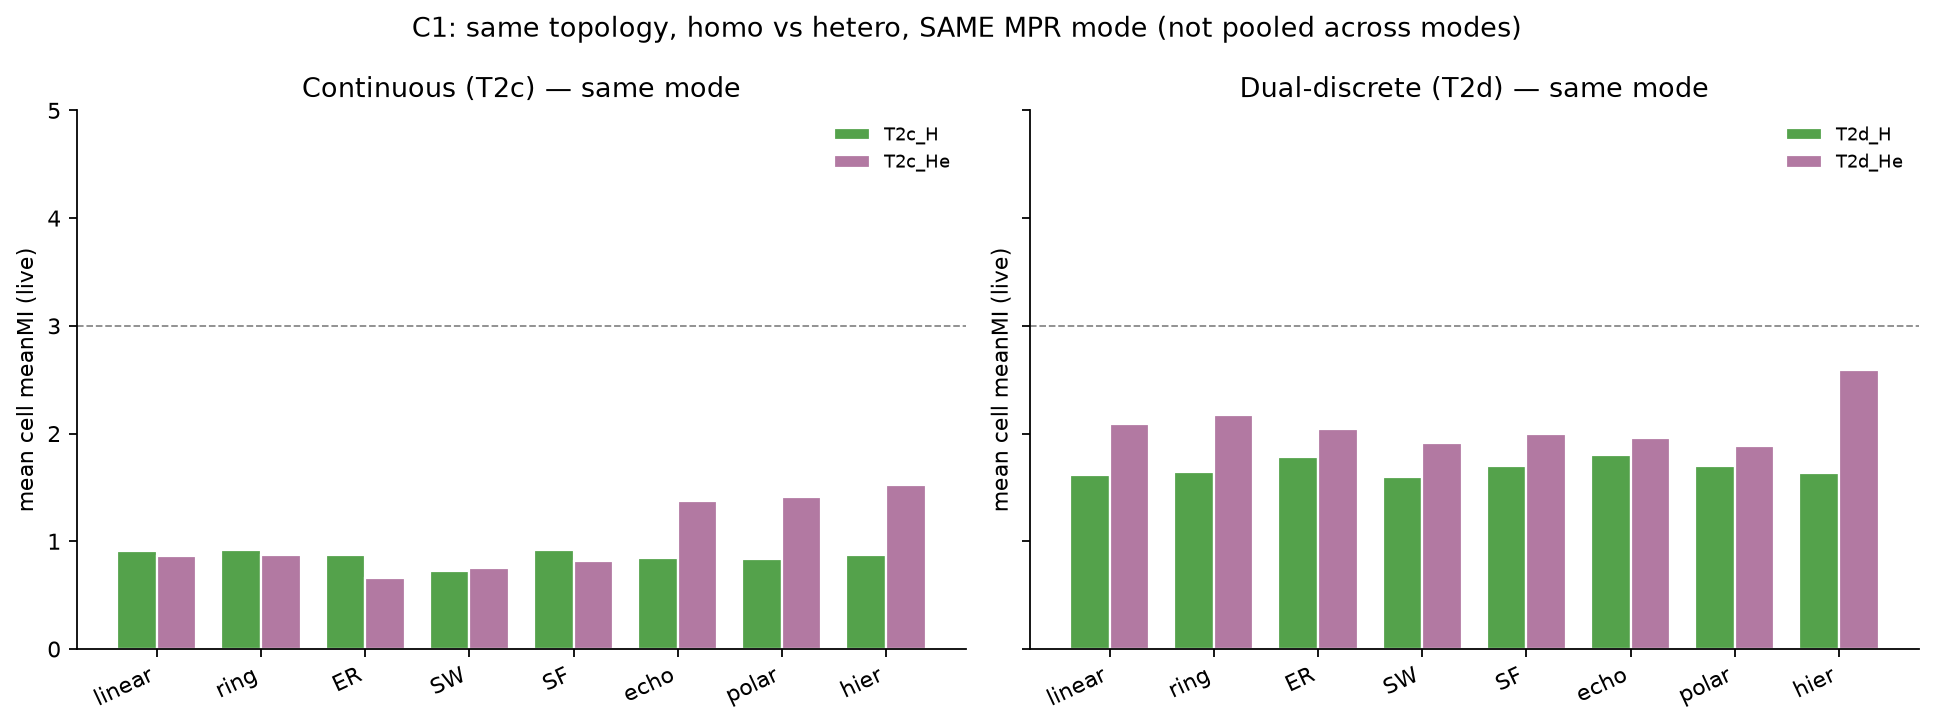
\includegraphics[width=\textwidth]{figures/fig01_c1_h_vs_he_same_mode.png}
\caption{C1 same-mode H and He live-cell means for all eight topologies.
Continuous and dual-discrete panels remain separate; dead cells are excluded
from means rather than set to zero.  $N=1$.}
\label{fig:c1-h-he}
\end{figure}

\begin{figure}[t]
\centering
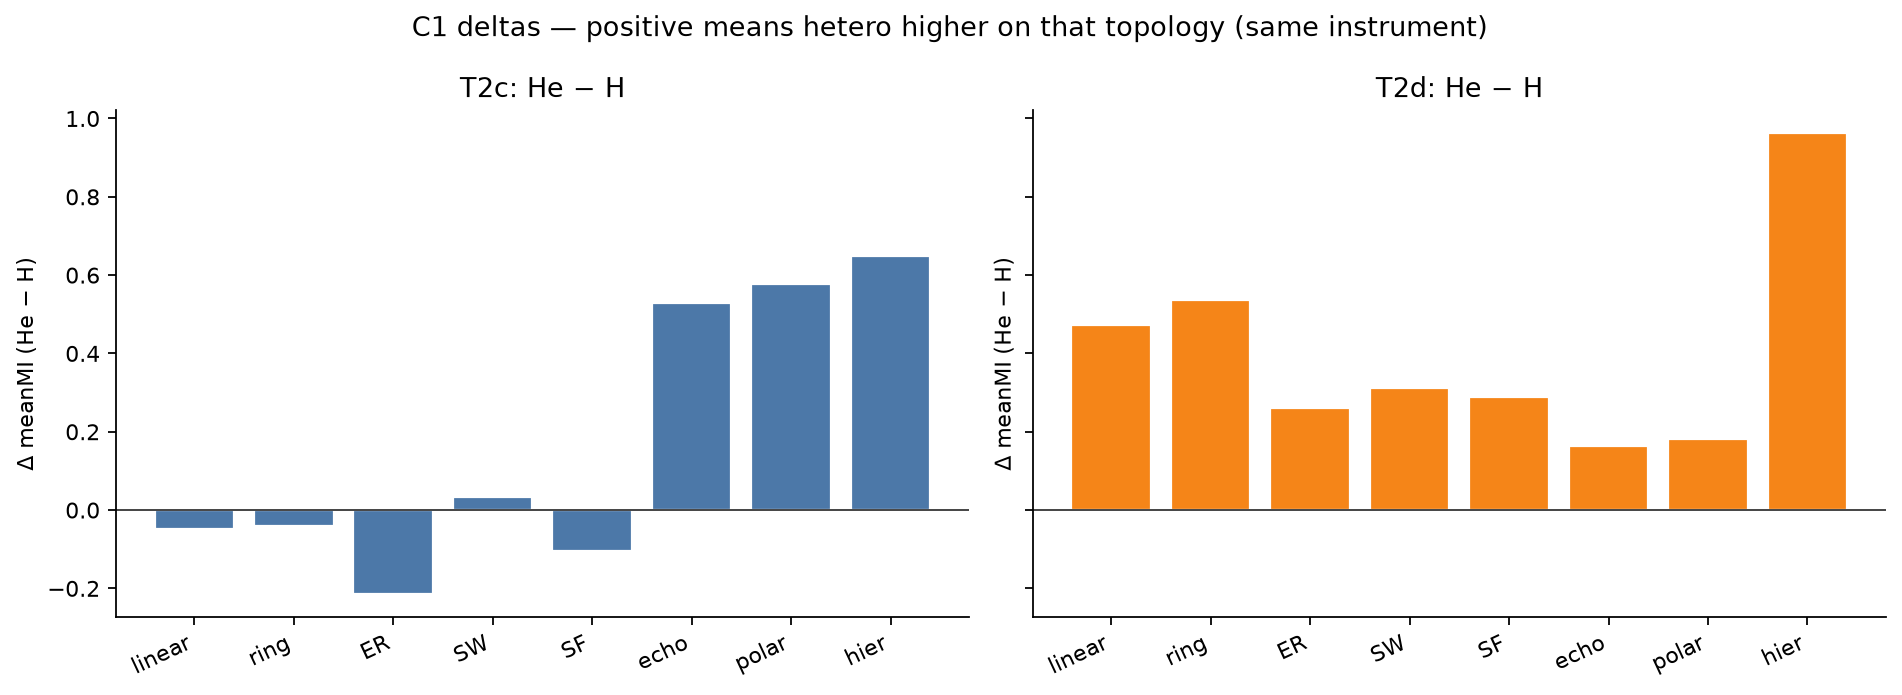
\includegraphics[width=\textwidth]{figures/fig02_c1_delta_he_minus_h.png}
\caption{C1 topology-level $\Delta(\mathrm{He}-\mathrm{H})$.  Continuous has
four positive and four negative differences; dual-discrete has eight positive
differences.  These are descriptive one-seed contrasts.}
\label{fig:c1-delta}
\end{figure}

The article-resolved topology pattern is shown in
\texttt{fig17\_topology\_article\_mpr.png}; topology-by-persona and
topology-by-mix views are in \texttt{fig15\_persona\_topology\_mpr.png} and
\texttt{fig16\_mix\_topology\_mpr.png}.  The corresponding denominators and
hatch pattern are visualised in \texttt{fig18\_dead\_rates.png}.  Those
figures should be read with the same live-only and mode-separation rules used
in the tables above.


\section{Results on the 63-node D-net}
\label{sec:results-dnet}

\subsection{Graph and persona placement}

The D-net experiments used the custom graph in
\path{thesisExperiment/data/derived/debnath_hashtag_cascade.json}.
It contains 63 nodes and 228 directed edges, collapsing to 171 unique
undirected pairs.  The nodes are accounts keyed by published hashtags and
the edges encode hashtag co-occurrence and same-cluster links.  Although the
edges occupy the importer's \texttt{retweets[]} field, they are not observed
retweets: Twitter/X hydration failed, and the object is not a retweet
cascade.  Both D-net persona conditions used exactly this topology and the
same seed node, \texttt{user\_chemtrails\_hub}.

The heterogeneous placement retained the reconstructed Debnath type mix.
Of the 63 placements, 56 used the exact reconstructed persona identifier.
The remaining seven used a coarser persona identifier while retaining the
mapped Debnath type:
\begin{itemize}
  \item \texttt{user\_depopulation\_amp}:
  \texttt{conspiracy\_depopulation} $\rightarrow$
  \texttt{conspiracy\_believer};
  \item \texttt{user\_climateaction\_piggyback\_amp} and
  \texttt{user\_climateaction\_piggyback\_peri\_1}:
  \texttt{conspiracy\_climate\_piggyback} $\rightarrow$
  \texttt{conspiracy\_believer};
  \item \texttt{user\_biodiversity\_hub},
  \texttt{user\_biodiversity\_peri\_1}, and
  \texttt{user\_foodsecurity\_amp}:
  \texttt{biodiversity\_food\_security} $\rightarrow$
  \texttt{environmental\_concern}; and
  \item \texttt{user\_mitigation\_amp}:
  \texttt{mitigation\_first\_policy} $\rightarrow$
  \texttt{climate\_action\_advocate}.
\end{itemize}
Thus the heterogeneous arm placed 28 conspiracy-family, 19
climate-action, 13 environmental, and three expert personas.  The
homogeneous arm instead assigned \texttt{conspiracy\_believer} to all 63
nodes.  The empirical hashtag identities were 28 conspiracy, 19
climate-action, 14 environmental-concern, and two other nodes; this
difference in counting reflects the coarser simulation placement, including
the type-only fallback for \texttt{user\_mitigation\_amp}, rather than a
change to the graph.

\subsection{Four D-net arms}

Four completed configurations crossed continuous versus dual-discrete
auditing with homogeneous conspiracy versus heterogeneous Debnath-mapped
personas.  Each configuration propagated two seed articles, producing the
eight article-level results in Table~\ref{tab:dnet-arms}.  These are
auditor scores from the simulation, not measurements made on Twitter.

\begin{table}[htbp]
\centering
\caption{Article-level auditor scores in the four D-net configurations.
The continuous sidecar from a dual run is shown only as a diagnostic and is
not interchangeable with the continuous-run headline.}
\label{tab:dnet-arms}
\small
\begin{tabular}{llrrr}
\toprule
Configuration & Article & Headline score & $n$ scored & Dual sidecar \\
\midrule
\texttt{Dnet\_c\_H\_conspiracy}
  & SCoPEx & 1.7349 & 970 & --- \\
\texttt{Dnet\_c\_H\_conspiracy}
  & chemtrails--Gates & 3.3378 & 984 & --- \\
\texttt{Dnet\_c\_He\_mixed}
  & SCoPEx & 0.9983 & 591 & --- \\
\texttt{Dnet\_c\_He\_mixed}
  & chemtrails--Gates & 2.5068 & 1,035 & --- \\
\texttt{Dnet\_d\_H\_conspiracy}
  & SCoPEx & 4.2537 & 1,076 & 2.2495 \\
\texttt{Dnet\_d\_H\_conspiracy}
  & chemtrails--Gates & 3.7303 & 749 & 3.1251 \\
\texttt{Dnet\_d\_He\_mixed}
  & SCoPEx & 2.6880 & 407 & 1.1302 \\
\texttt{Dnet\_d\_He\_mixed}
  & chemtrails--Gates & 1.5297 & 1,027 & 1.1497 \\
\bottomrule
\end{tabular}
\end{table}

Within each article and instrument, homogeneous conspiracy scored above the
mixed placement: 1.7349 versus 0.9983 and 3.3378 versus 2.5068 under the
continuous auditor, and 4.2537 versus 2.6880 and 3.7303 versus 1.5297 under
the dual-discrete auditor.  Article ordering depended on the instrument.
Chemtrails--Gates exceeded SCoPEx in both continuous arms, whereas SCoPEx
exceeded chemtrails--Gates in both dual-discrete arms.

\subsection{Do the small-topology findings hold?}

Only the composition result transfers cleanly.  In the eight-node grid,
conspiracy-family homogeneous cells were the high-score family on both
instruments (3.1691 dual-discrete and 2.2194 continuous).  The D-net result
is consistent with that finding: replacing the mixed type placement with
63 conspiracy-believer seats raised the score for both articles under both
auditors.

The collapsed H/He result does not transfer as an H/He law.  Across the
eight small topologies, collapsed He exceeded collapsed H by 0.1549 under
continuous scoring and by 0.3986 under dual-discrete scoring, although the
continuous He$>$H ordering held on only four of the eight individual
topologies.  On D-net, H exceeded He in all four like-for-like article and
instrument comparisons.  This reversal is consistent with the different
composition of the labels: small-topology H pooled conspiracy personas with
scientists, while D-net H means conspiracy-only.

Nor does the small-grid instrument ordering hold without exception.  The
eight-topology aggregates placed dual-discrete above continuous on every
topology.  On D-net, the dual headline exceeded the corresponding
continuous-run headline for homogeneous SCoPEx, homogeneous
chemtrails--Gates, and mixed SCoPEx, but not for mixed
chemtrails--Gates (1.5297 dual-discrete versus 2.5068 continuous).
Because these are different auditors, even the three concordant
comparisons are instrument differences rather than estimates in a shared
unit.  D-net has only one fixed 63-node topology, so it cannot replicate or
rank the eight small topology treatments.

\subsection{Auditor MI is not empirical Twitter MPR}

Debnath provides no empirical 0--5 misinformation-propagation-rate
(\textsc{mpr}) outcome for this graph.  The source tweet identifiers were
not hydrated, the graph has no empirical tweet clock, and no tweet-level
content score can be paired with a simulated event.  Accordingly, the
values in Table~\ref{tab:dnet-arms} are LLM-as-judge auditor misinformation
indices (\textsc{mi}) inside the simulation.  They must not be described as
Twitter \textsc{mpr}, as Twitter \textsc{mi}, or as a match to observed
misinformation.  The dual-discrete headline, its continuous sidecar, and
the continuous-only headline are also separate instruments and are not
averaged.

\subsection{Structural comparison and validation diagnostics}

The copied graph has global transitivity 0.3146, mean local clustering
0.5153, and mean unique degree 5.4286.  The
\texttt{user\_chemtrails\_hub} node has 33 unique neighbours.  Using
unweighted unique-undirected pairs, the mixed-label conspiracy cut has
Newman--Girvan modularity 0.4297; the homogeneous one-community partition
has modularity 0.  Mixed-label identity homophily is 0.8377
in the simulation; homogeneous identity homophily is 1.0 by construction,
so the latter is not evidence of an emergent echo chamber.

For the rooted cascade-shape comparison, the empirical object had depth
4, breadth 33, reached size 61, and structural virality 2.7.  Across 16
simulated D-net cascades, the corresponding means were 2.5625, 40.9375,
53.5, and 1.7963.  Breadth was the only one of the three validation metrics
(depth, breadth, and structural virality) within the pre-specified
30\% band; the resulting structural-similarity score was 0.6885.

The distributional diagnostics do not validate a digital twin.
With one empirical object and 16 simulated cascades, the
Kolmogorov--Smirnov results were $D=1.0000$, $p=0.1104$ for depth;
$D=0.8125$, $p=0.2954$ for breadth; and $D=1.0000$, $p=0.1104$ for
structural virality.  Jensen--Shannon divergence was 1.0000 for all three
metrics, and all three distribution-match flags were false.  The empirical
sample size of one makes the KS comparisons underpowered; their
non-significant $p$-values are not evidence of equivalence.  Finally, DTFS
was 0.2754, below the 0.70 validation threshold
(\texttt{isValidated=false}).  Its content-correlation component was fixed
at zero because no empirical \textsc{mpr} or tweet-text \textsc{mi} exists.
The structural evidence therefore supports a comparison of cascade shape,
not empirical misinformation fidelity or digital-twin validation.


\section{Applying the Pfeffer firestorm framework}
\label{sec:pfeffer-application}

\subsection{The original framework and the thesis remapping}

\Textcite{pfeffer2014firestorms} define an online firestorm as a sudden
discharge of large quantities of negative word-of-mouth and complaint
messages directed at a person, company, or group.  The messages are
predominantly opinion rather than fact and are therefore highly affective.
The article is a qualitative--synthetic account based on observed cases; it
does not present an agent-based model, a tipping-point estimator, or a
climate-discourse experiment.

The Outlook of \textcite{pfeffer2014firestorms} identifies seven
interrelated factors:
\begin{enumerate}
    \item \emph{speed and volume of communication};
    \item \emph{binary choices};
    \item \emph{network clusters};
    \item \emph{unrestrained information flow};
    \item \emph{lack of diversity};
    \item \emph{cross-media dynamics}; and
    \item \emph{network-triggered decision processes}.
\end{enumerate}
These are the original factors used here.  In particular, valence and
surprise are not numbered Outlook factors.  Valence is motivated by the
affective character in the paper's definition of a firestorm, while surprise
is a thesis operationalisation of the novelty, speed, and volume mechanism in
factor~1.

The thesis vocabulary---valence, surprise, identity, clustering, echo,
temporal, and cross-media---is consequently a computational remapping, not a
renaming of Pfeffer et al.'s list.  The first six terms describe variables or
observables that can at least partly be represented in the simulation;
cross-media is included as a seventh ledger row but is held because the model
has no legacy-media layer.  Conversely, Pfeffer et al.'s binary-choice factor
has no dedicated thesis row.  The agents choose among
\texttt{forward}, \texttt{reinterpret}, and \texttt{drop}, so the engine is
ternary rather than an implementation of the paper's like/share/retweet
either--or mechanism.

\begin{table}[t]
\centering
\caption{Original Outlook factors and their treatment in the thesis.  The
right-hand column is an operational mapping, not Pfeffer et al.'s
terminology.}
\label{tab:pfeffer-original-remap}
\small
\begin{tabular}{p{0.05\textwidth}p{0.32\textwidth}p{0.53\textwidth}}
\toprule
\# & Pfeffer et al.\ (2014) & Thesis treatment \\
\midrule
1 & Speed and volume of communication
  & Surprise (shock versus drip) and temporal horizon; surprise is held at
    drip and empirical timing is unavailable. \\
2 & Binary choices
  & No dedicated observable or sweep; simulated actions are ternary. \\
3 & Network clusters
  & Clustering and part of the echo measurement. \\
4 & Unrestrained information flow
  & Partly represented by echo and hub reach, but not the hundreds or
    thousands of weak ties discussed in the paper. \\
5 & Lack of diversity
  & Identity composition and part of echo/homophily; homogeneous versus
    mixed belief profiles are compared. \\
6 & Cross-media dynamics
  & Held; neither the empirical reconstruction nor the engine contains a
    legacy-media or newsroom layer. \\
7 & Network-triggered decision processes
  & Related to the temporal ledger row, but the four adoption stages are not
    logged or estimated. \\
\bottomrule
\end{tabular}
\end{table}

\subsection{Order of application: empirical structure before simulation}

The application proceeds in two distinct stages.  First, structural
observables are calculated on the empirical fallback derived from
\textcite{debnath2023conspiracy}.  This object is a hashtag co-occurrence
graph with 63 nodes, 228 directed edges, and 171 unique undirected pairs.
It is not a retweet, reply, follower, or \texttt{conversation\_id} cascade.
The 814,924 tweet identifiers in the associated dataset were not hydrated,
and the graph contains no usable tweet clock.  Its labels and edges can
therefore support a bounded comparison of hashtag structure, but not a
reconstruction of user-to-user diffusion.

Second, D-net imports the same 63-node, 228-edge topology and runs agents on
it.  This ordering matters: transitivity, local clustering, hub degree, and
the mixed-label conspiracy cut already exist before any simulated message is
generated.  D-net copies this structure; it does not produce or validate it.
The post-simulation evidence consists of content-auditor scores, realised
actions and reach on that fixed graph, together with label-dependent
quantities for the homogeneous and mixed assignments.

\paragraph{Empirical hashtag structure.}
The graph has global transitivity \(0.315\), mean local clustering \(0.515\),
and mean unique degree \(5.43\).  The \texttt{\#chemtrails} hub has 33 unique
neighbours.  On the 171 unique-undirected pairs, the six assigned graph
clusters have \(Q=0.5489\), the four assigned discourse identities have
\(Q=0.5322\), and the binary conspiracy cut has \(Q=0.4297\).
These label-partition statistics are distinct from clustering coefficients.
Identity edge homophily is \(0.873\);
belief-profile-family homophily is \(0.838\).  The identity composition is
28 conspiracy, 19 climate-action, 14 environmental, and two expert/other
nodes.  Thus conspiracy discourse is a plurality (\(28/63=0.444\)), not a
monoculture.

\paragraph{D-net after simulation.}
The mixed D-net condition retains 28 conspiracy nodes and the empirical
type-level composition, with 19 climate-action, 13 environmental, and three
expert nodes after belief-profile assignment.  The homogeneous condition
instead assigns all 63 seats the
\texttt{conspiracy\_believer} profile.  Because both conditions use the same
edge set, transitivity, local clustering, and hub degree remain \(0.315\),
\(0.515\), and 33.  Mixed D-net identity homophily is \(0.838\), whereas the
homogeneous value is \(1.0\) by construction.  The latter is not evidence
that an echo chamber emerged.  It is the mechanical result of giving every
node the same identity.  Mixed belief-profile families have \(Q=0.4908\),
and the mixed binary conspiracy cut has \(Q=0.4297\).  Under homogeneous
labels there is only one community, for which \(Q=0\).

Across the four primary D-net cells, 61 of 63 nodes receive a message within
the held eight-tick horizon.  This demonstrates reach under the engine's
rules on the imported graph.  It does not establish that the empirical
Twitter discourse spread to 61 users in eight equivalent units of time.
Simulation ticks have no defensible conversion to hours, and the eight-hop
budget is a computationally compressed horizon.

\subsection{What the application can and cannot reveal}

\begin{table}[t]
\centering
\caption{Interpretive boundary of the Pfeffer application.  Empirical values
refer to the hashtag graph before simulation; simulated values refer to
D-net after a run.}
\label{tab:pfeffer-reveal-limits}
\scriptsize
\begin{tabular}{p{0.12\textwidth}p{0.36\textwidth}p{0.42\textwidth}}
\toprule
Observable & What the method reveals & What the method cannot reveal \\
\midrule
Clustering
& Before simulation, the hashtag construction contains substantial closure:
  transitivity \(0.315\), local clustering \(0.515\), and a hub of degree
  33.  The mixed-label cut has \(Q=0.404\).
& These values are not retweet triadic closure or emergent D-net clusters.
  The graph is a documented co-occurrence construction, not a
  Watts--Strogatz fit, and previously reported Debnath eigenvector
  centralities were not re-estimated here. \\

Echo
& Empirical identity homophily \(0.873\) and belief-profile-family
  homophily \(0.838\) show that most represented ties remain within discourse
  blocks.  Mixed D-net retains comparable block echo
  (\(0.838\)).
& The measure does not identify algorithmic ranking, weak-tie exposure, or
  an emergent chamber.  Homogeneous D-net homophily of \(1.0\) is tautological
  and cannot measure echo formation. \\

Identity
& The comparison separates a mixed empirical-type composition
  (conspiracy share \(0.444\)) from the homogeneous intervention
  (share \(1.0\)).  It therefore isolates identity composition as a model
  input on a common topology.
& The labels are theory-grounded reductions, not HDBSCAN communities
  recovered from hydrated tweets, and they do not establish individual
  users' identities or follower-network homophily. \\

Valence proxy
& The empirical side supplies only the paper-reported toxicity mean
  (approximately \(0.17\)) and a hashtag prior proxy (\(0.1097\)); the
  simulated side supplies an LLM-auditor misinformation index.  On the
  continuous instrument, the chemtrails seed has higher mean \(\mathrm{MI}\)
  than the SCoPEx seed in both homogeneous and mixed D-net.
& Toxicity, a hashtag prior, and auditor \(\mathrm{MI}\) are different
  constructs and scales.  Debnath provides no empirical \(\mathrm{MPR}\).
  The comparison cannot be described as Twitter \(\mathrm{MI}\), an
  empirical-to-simulated \(\mathrm{MPR}\) match, or validation of a
  firestorm. \\

Surprise
& The ledger records the seeded regime: a single
  \texttt{user\_chemtrails\_hub} provides drip seeding.  The
  paper-reported SCoPEx volume spike motivates the construct.
& Surprise is held, not tested.  There is no all-node shock condition and no
  reconstructed empirical volume series, novelty half-life, or attention
  decay. \\

Temporal
& D-net records engine progression for eight ticks and shows 61/63-node
  reach within that budget.
& Empirical timing is unavailable because the hashtag fallback has no tweet
  clock.  Ticks cannot be translated into minutes or hours, and the method
  cannot estimate inter-arrival times, half-life, or Pfeffer et al.'s
  knowledge--persuasion--propagation--affirmation sequence. \\

Cross-media
& The ledger makes the omission explicit rather than attributing it to a
  topology.
& Cross-media dynamics are held on both sides.  There is no social-to-legacy-
  media-to-social loop, newsroom agent, external-volume estimate, or basis
  for treating a hierarchical graph as cross-media amplification. \\
\bottomrule
\end{tabular}
\end{table}

The valence result requires particular care.  In the continuous runs, mean
auditor \(\mathrm{MI}\) for SCoPEx is \(1.735\) in homogeneous D-net and
\(0.998\) in mixed D-net; for the chemtrails seed it is \(3.338\) and
\(2.507\), respectively.  These values show content degradation under a
particular auditor and graph intervention.  They do not measure indignation
or toxicity.  The dual-discrete instrument is a separate scale and does not
preserve the same article ordering in every cell, so the two instruments are
not averaged.

Likewise, the network-mean threshold \(k^*\), where used, is a thesis rule
based on simulated \(\mathrm{MI}\).  It is neither a statistic introduced by
\textcite{pfeffer2014firestorms} nor an empirical estimate from
\textcite{debnath2023conspiracy}.  Structural cascade comparison also does
not repair this gap: the available comparison has one empirical graph, and
its reported digital-twin fit score is \(0.2754\), below the \(0.70\)
validation threshold.  The D-net application should therefore be read as a
controlled, theory-mapped simulation on an empirical structural stand-in,
not as a validated digital twin of the geoengineering conversation.

\subsection{Interpretation}

The application supports three bounded conclusions.  First, clustering and
block homophily are properties of the empirical hashtag representation
before simulation; they are consistent with the structural mechanisms in
Pfeffer et al.'s factors 3 and 5, but do not prove a user-level firestorm.
Second, holding topology fixed while changing the belief-profile
composition distinguishes mixed from homogeneous D-net outcomes and avoids
mistaking an all-identical assignment for emergent echo.  Third, content
auditing can describe simulated factual degradation after propagation, but
it cannot supply the missing empirical temporal, binary-choice, weak-tie, or
cross-media processes.  The framework is thus applied as an explicit
mapping and limitation ledger, not as a claim that all seven original
factors were experimentally realised.
\fussy

\chapter{Discussion}
\label{chap:discussion}

This chapter interprets the Phase~2 results in relation to the research
questions and the literature.  The distinction between evidence,
interpretation, and implication is maintained throughout.  This distinction is
necessary because the campaign comprises one run per configuration
($N=1$), one graph seed, an eight-tick horizon, and 292 dead cells among
1,728 configured cells.  The reported quantities are therefore descriptive
properties of the present LLM simulation.  They are neither estimates of
population effects nor measurements of misinformation on Twitter.

\section{Synthesis of the research questions}
\label{sec:discussion-rqs}

\subsection{RQ1: What does the instrument comparison establish?}

The measurement result precedes all substantive comparisons. Dual-discrete scores exceeded continuous scores on every topology in both arms, while topology ranks aligned weakly. The campaign therefore shows that MI and MPR conclusions depend on the auditor regime. This finding answers RQ1: neither instrument can serve as an unqualified ground truth, and cross-mode pooling is not admissible.

\subsection{RQ3: How does network topology affect misinformation
propagation?}

\paragraph{Evidence.}
Topology changed the live-cell scores, the frequency of irreversible
\kstar{}, and the probability that a cascade remained scorable.  However, no
topology occupied the highest or lowest position consistently across identity
composition and scoring instrument.  In homogeneous continuous runs,
scale-free networks had the highest topology mean ($0.9205$), whereas
small-world networks had the lowest ($0.7215$).  In homogeneous
dual-discrete runs, echo chambers had the highest mean ($1.7984$), again with
small-world networks lowest ($1.5977$).  In heterogeneous runs, the
hierarchical topology had the highest mean under both instruments ($1.5242$
continuous and $2.5934$ dual-discrete).  These latter estimates must be read
together with the hierarchical dead-cell rates of $27.8\%$ and $22.2\%$,
respectively.  Polarised heterogeneous continuous runs likewise combined a
high live-cell mean ($1.4137$) with a $30.6\%$ dead-cell rate.

\paragraph{Interpretation.}
The results do not support a topology-invariant ranking.  Topology appears to
condition which messages are observed and scored, but it does so jointly with
persona placement, article content, and cascade survival.  In particular,
live-only means on topologies with many dead cells describe the surviving
cascades rather than the generator as a whole.  The scale-free versus random
comparison is primarily a hub and degree-sequence contrast; it is not a
controlled comparison of clustering coefficients.  Similarly, the
hierarchical generator represents authority-oriented transmission and should
not be interpreted as a model of cross-media dynamics.

\paragraph{Implication.}
Topology should be treated as a conditioning structure, not as a sufficient
cause of factual degradation.  Subsequent work should use repeated graph
seeds, report cascade survival as an outcome, and match graph properties when
isolating a specific mechanism such as clustering, centralisation, or
community separation.  On the present evidence, selecting a single
\enquote{most harmful} topology would overstate what the design identifies.

\subsection{RQ2: What is the role of identity composition?}

\paragraph{Evidence.}
When all eight generated topologies were collapsed within one instrument, the
heterogeneous arm exceeded the homogeneous arm: by $0.1549$ in continuous
\MI{} (H $0.8643$, He $1.0192$) and by $0.3986$ in dual-discrete \MI{}
(H $1.6814$, He $2.0800$).  The continuous direction was nevertheless split:
He exceeded H on four of eight topologies, whereas H exceeded He on the other
four.  The dual-discrete direction was He$>$H on all eight topologies.
Composition-specific results were substantially more differentiated than
these arm labels.  Homogeneous conspiracy-family cells reached $2.2194$
continuous and $3.1691$ dual-discrete, compared with $0.1118$ and $0.8687$
for homogeneous science/environment personas.  Among heterogeneous mixes,
\texttt{mix\_00}, containing four conspiracy personas, scored $1.7712$
continuous and $3.1321$ dual-discrete; conspiracy-free \texttt{mix\_02}
scored $0.2645$ and $1.1882$.

\paragraph{Interpretation.}
The collapsed H/He contrast is not an estimate of a general effect of
diversity.  The homogeneous arm contains both conspiracy-only and
scientist-only societies, while the heterogeneous arm contains mixes with
different conspiracy shares and different persona identities.  Averaging
within these broad labels changes the distribution of substantive roles.
Consequently, the observed He$>$H collapse is compatible with a strong
composition gradient: conspiracy-conditioned cells score high, whereas
science-conditioned cells score low.  It does not establish that
heterogeneity intensifies misinformation, just as the low value of
\texttt{mix\_02} does not establish that diversity prevents it.

\paragraph{Implication.}
Future comparisons should hold the proportion and identity of
conspiracy-conditioned seats constant while varying only within-network
diversity or placement.  Network means should be accompanied by
persona-conditioned \MPR{} and exposure-matched comparisons.  This would
separate a genuine interaction between heterogeneous neighbours from the
mechanical dilution or enrichment produced by changing the number of
high-scoring personas.

\subsection{Measurement implications across RQ2 and RQ3}

\paragraph{Evidence.}
Dual-discrete scores exceeded continuous scores on all eight topologies in
both arms.  The topology-mean difference was $0.8201$ for homogeneous and
$1.0450$ for heterogeneous runs.  Among cells live under both modes, the
median paired difference was $0.8125$ for H ($n=398$) and $0.9778$ for He
($n=198$).  Instrument choice also affected the incidence of irreversible
\kstar{}: the collapsed He rates were $32.1\%$ under dual-discrete scoring and
$7.6\%$ under continuous scoring.  Moreover, topology rankings agreed only
weakly across modes in the exploratory analysis (Spearman
$\rho=0.095$ for H and $\rho=0.167$ for He).

\paragraph{Interpretation.}
The two modes are not interchangeable measurements on a common numerical
scale.  The discrete instrument awards categorical penalties for omitted or
contradicted answers, whereas the continuous instrument resolves degradation
differently.  The systematic level difference and weak rank agreement show
that instrument choice can affect both absolute severity and comparative
claims about topology.  The continuous sidecar generated during a dual run is
useful for diagnosing disagreement, but it is not a third independent
\MPR{}.

\paragraph{Implication.}
Substantive conclusions should be reported separately for each instrument.
Averaging the two modes would create a quantity without a defined auditor.
The disagreement also motivates external validation: a preregistered sample
of rewrites should be assessed by human coders, and calibration should examine
whether each instrument preserves article- and persona-level ordering rather
than merely correlating at the event level.  Until such validation is
available, \kstar{} is instrument-relative.

\subsection{RQ4: Does the D-net analysis generalise the generated-topology
findings?}

\paragraph{Evidence.}
D-net used a 63-node custom graph reconstructed from hashtag co-occurrence,
not a retweet cascade.  Its homogeneous condition assigned
\texttt{conspiracy\_believer} to all 63 seats; its mixed condition retained a
conspiracy share of $28/63$.  On the identical edge set, homogeneous
conspiracy exceeded the mixed condition for both articles and both
instruments: continuous SCoPEx $1.7349$ versus $0.9983$, continuous
chemtrails--Gates $3.3378$ versus $2.5068$, dual-discrete SCoPEx $4.2537$
versus $2.6880$, and dual-discrete chemtrails--Gates $3.7303$ versus
$1.5297$.  Structural comparison was less favourable.  Breadth fell within
the specified $30\%$ band, whereas depth and structural virality did not;
DTFS was $0.2754$ and failed the $0.70$ validation threshold.  Tests comparing
one empirical graph with 16 simulated cascades were underpowered.

\paragraph{Interpretation.}
D-net provides a useful stress test of the composition interpretation because
the topology is held fixed while persona labels change.  It does not provide
out-of-sample validation of the eight-node generators, and it is not a
digital twin of Debnath et al.'s Twitter corpus.  The graph imports
co-occurrence structure and then simulates message propagation on that
structure; it neither reconstructs empirical retweet paths nor reproduces an
empirical misinformation score.  The D-net result therefore supports the
narrow statement that a conspiracy-only assignment scored above the retained
mixed assignment on this larger custom graph.

\paragraph{Implication.}
The qualitative composition gradient travels from the generated graphs to
D-net, but numerical effect sizes and cascade-shape claims do not.  Stronger
generalisation would require hydrated interaction data, common community and
centrality estimators, temporal information, multiple reconstructed cascades,
and repeated simulation seeds.  Simulated auditor \MI{} must remain separate
from Debnath et al.'s toxicity and network measures
\parencite{debnath2023conspiracy,ruths2014social}.

\section{Reconciling the collapsed and D-net orderings}
\label{sec:discussion-reconciliation}

\paragraph{Evidence.}
The generated-topology collapse gives He$>$H. In D-net, homogeneous
conspiracy scores exceed the mixed assignment. These comparisons use
different definitions of H.
Across the eight-node grid, H denotes twelve separate homogeneous persona
societies, including four conspiracy personas as well as climate-action,
environmental, journalist, and scientist personas.  D-net H denotes one
specific treatment: all 63 nodes are assigned the
\texttt{conspiracy\_believer} persona.  D-net He preserves a majority
non-conspiracy composition.  Restricting the generated-topology H cells to
the conspiracy family already reverses the broad collapse: conspiracy H is
well above overall He on both instruments.

\paragraph{Interpretation.}
There is therefore no empirical contradiction to resolve.  The label H
encodes within-network uniformity, but it does not encode which identity is
uniform.  Collapsing across homogeneous scientist and homogeneous conspiracy
societies answers a different question from comparing a conspiracy monoculture
with a mixed society.  D-net changes both diversity and the prevalence of the
high-scoring persona when moving from H to He.  Its ordering is consequently
consistent with composition, but cannot distinguish composition from a
causal benefit of heterogeneity.

\paragraph{Implication.}
H and He should not be used as portable substantive treatments without an
attached composition descriptor.  A defensible notation would distinguish,
for example, H-conspiracy, H-science, He-44\%-conspiracy, and
He-0\%-conspiracy.  A matched factorial design could then vary diversity while
holding conspiracy share, seed position, and topology fixed.  This
reformulation is more informative than asking whether H or He is
\enquote{higher} in the abstract.

\section{Relation to the award paper and adjacent literature}
\label{sec:discussion-literature}

\subsection{The CIKM/LASS study as prior method, not a benchmark result}

\paragraph{Evidence from the literature.}
\textcite{maurya2025simulating} introduced the auditor--node framework, MI and
MPR, and the severity taxonomy used by the present system.  Its published
evaluation concerned 30-hop linear branches, a different article collection,
a larger persona inventory, ten auditor questions, and a different model
configuration.  It reported that identity- and ideology-oriented homogeneous
branches could accelerate degradation and that experts could stabilise it;
it also reported propaganda-tier outcomes in approximately $85\%$ of
heterogeneous branch--domain pairs.  Thus, the award paper itself does not
establish a universal rule that heterogeneous societies must score below
homogeneous societies.

\paragraph{Interpretation of the present comparison.}
The present study transfers the instrument to climate and geoengineering
content and extends the setting from linear branches to generated and custom
graphs.  The non-zero, persona-sensitive scores indicate that the instrument
remains responsive in this domain.  The observed collapsed He$>$H ordering is
not a failed replication of a universal CIKM H$>$He hypothesis, because no
such universal hypothesis follows from the prior heterogeneous result.
Conversely, D-net H-conspiracy$>$He-mixed cannot be presented as a
replication: identity inventories, graph objects, hop budgets, auditor
questions, and model settings differ, and the present campaign has only one
replicate.

\paragraph{Implication.}
The defensible contribution is a boundary analysis of the prior method, not a
numerical reproduction of the award paper.  A direct conceptual replication
would require matched linear chains, an expert-inclusive heterogeneous arm,
the same climate articles in both arms, a sufficiently broad article set, and
node-type-conditioned outcomes.  The eight-hop graph campaign can motivate
that test but cannot substitute for it.

\subsection{Topology and diffusion literature}

\paragraph{Evidence from the literature.}
Classical diffusion models establish that network structure affects reach and
activation opportunities \parencite{kempe2003influence}.  Small-world and
preferential-attachment models formalise different structural properties
\parencite{watts1998collective,barabasi1999emergence}.  Empirical work further
shows that cascade depth and breadth are not captured by size alone
\parencite{goel2016virality}, and that false news can diffuse farther and
faster than true news in observational data \parencite{vosoughi2018false}.

\paragraph{Interpretation of the present comparison.}
The present results are compatible with the general proposition that
structure conditions diffusion, but they do not re-estimate these empirical
findings.  Here the state is mutable text, forwarding is mediated by an LLM,
and live-cell \MI{} is an auditor output.  Topology effects are also entangled
with cascade death and composition.  The data therefore add a
content-transformation perspective to network diffusion; they do not show
that one canonical graph class is intrinsically most susceptible to
misinformation.

\paragraph{Implication.}
Network controls in LLM societies should include both structural summaries
and content outcomes.  Matching degree, density, seed centrality, and
clustering would permit more specific tests than topology names alone.

\section{Pfeffer's firestorm theory: insights and boundaries}
\label{sec:discussion-pfeffer}

\paragraph{Evidence.}
\textcite{pfeffer2014firestorms} identify seven interrelated factors: speed
and volume of communication, binary choices, network clusters, unrestrained
information flow, lack of diversity, cross-media dynamics, and
network-triggered decision processes.  The present six-knob vocabulary is a
computational remapping rather than this original list.  The campaign varied
network structure and identity composition and compared article frames.  It
held surprise as a single-node drip, fixed the horizon at eight ticks, omitted
a cross-media layer, and used ternary actions---forward, reinterpret, and
drop---rather than binary platform actions.  D-net's empirical structure had
transitivity $0.315$, mean local clustering $0.515$, and mixed-label
homophily close to $0.84$, but these structures were pre-wired rather than
generated by the simulation.

\paragraph{Interpretation.}
Two Pfeffer insights receive limited support as useful design principles.
First, network clusters and identity structure cannot be reduced to a single
topology label: the high-scoring composition can be concentrated or diluted
within the same graph.  Second, lack of diversity is not adequately tested by
the binary H/He label unless identity prevalence is controlled.  The D-net
comparison illustrates both points particularly clearly.  By contrast, this
campaign does not test speed and volume as a shock manipulation,
unrestrained information flow at platform scale, binary-choice dynamics,
cross-media amplification, or the four stages of network-triggered adoption.
Nor does \kstar{} originate in Pfeffer's framework; it is a thesis-specific
auditor threshold.

\paragraph{Implication.}
Pfeffer's framework is most productive here as an audit of what the
simulation represents and omits.  It should not be presented as a
seven-factor confirmation.  A fuller test would add shock versus drip
seeding, a binary-action ablation, a legacy-media or exogenous-broadcast
layer, and explicit logging of repeated exposure and affirmation.  Such
extensions would move the framework from retrospective mapping towards
identified mechanism tests.

\section{Alternative explanations and validity of the interpretation}
\label{sec:discussion-validity}

Several alternative explanations remain plausible.  Persona prompts may
induce role compliance rather than persistent beliefs; high conspiracy scores
may therefore partly measure how faithfully the model follows an instruction
to use conspiratorial language.  The action policy gives reinterpretation a
substantial role, which creates opportunities for factual mutation by design.
The same model family participates in generation and automated assessment,
and the five author-defined questions constrain what counts as degradation.
Article differences combine topic, wording, affective charge, and prior fit
with persona prompts, so they are not a clean manipulation of valence.
Finally, excluding dead cells from means avoids coding them as factual zeros,
but produces survivor-conditioned estimates.

These limitations do not make the campaign uninformative.  They narrow the
appropriate claim.  The experiment demonstrates that, under the documented
prompts and graph protocols, auditor scores vary with persona composition,
topology, and scoring mode.  It does not establish human susceptibility,
platform-level firestorm dynamics, or causal effects in an empirical
population.  Human evaluation, model ablations, repeated seeds, and a
fail-closed auditor are therefore validation requirements rather than
optional refinements \parencite{zheng2023judge,park2023generative}.

\section{Overall implications}
\label{sec:discussion-implications}

For simulation methodology, the principal implication is that treatment
labels must preserve their substantive content.  \enquote{Homogeneous} and
\enquote{heterogeneous} are insufficient without persona shares, placement,
and node-conditioned outcomes.  Likewise, topology names should be
accompanied by realised graph statistics and cascade-survival rates.

For measurement, discrete and continuous \MI{} should be treated as separate
operationalisations.  Agreement in a direction across both instruments is
stronger descriptive evidence than a result present under only one, but
neither becomes ground truth through convergence.  Divergence is itself a
result about the sensitivity of the conclusion to the auditor.

For empirical generalisation, D-net is an intermediate case: larger and
structurally grounded in a hashtag graph, yet still neither a retweet cascade
nor a temporal reconstruction.  Its contribution is to show that the
composition interpretation survives a change in graph size and source under
the same simulator.  It does not validate the simulator against Twitter.

Taken together, the research questions yield a restrained conclusion.
Topology conditions propagation but has no stable winner; identity
composition is more informative than the H/He label; severity and \kstar{}
are instrument-dependent; and D-net supports only qualitative, not numerical,
generalisation.  Pfeffer's framework explains why these dimensions should be
considered jointly, while also making visible the mechanisms that the current
campaign leaves untested.

\chapter{Validity, Ethics, and Reproducibility}
\label{chap:limitations}

The Phase~2 results describe one configured simulation campaign. They are not
population estimates and not a validated digital twin of online climate
discourse. The harvest is therefore diagnostic: it shows which patterns
appeared under the specified graph generators, personas, articles, language
model, and scoring instruments, and where those patterns are sensitive to
design choices and API availability.

\section{Internal and statistical validity}

\paragraph{One replicate.}
The parser retained one run per configuration ($N=1$). Configurations
recorded \texttt{graphRandomSeed: 42}, but only the echo-chamber and polarised
builders consumed it; ER, small-world, scale-free, and action sampling used
unseeded \texttt{Math.random}. Article cells within a configuration share the
realised graph, persona assignment, protocol, and hosted-model context, so they
are not independent campaign replicates. Inboxes and per-article histories
were cleared between articles, and post-hoc trust updates could not alter
already completed trajectories.  The reported means and rank orders are
descriptive comparisons of this harvest; they do not provide confidence
intervals, population-level significance tests, or causal estimates of a
topology or identity-mix effect.  In particular, a small \(p\)-value computed
over pooled cells would not repair the absence of independent simulation
replicates.

\emph{Mitigation.}  Results are separated by scoring mode and accompanied by
live-cell counts and dead-cell rates.  Claims are phrased as observations
\enquote{in this harvest}, and the analysis avoids interpreting event counts
as sample size.  Future work should run independently seeded graph and model
replicates, predefine topology-level contrasts, and estimate uncertainty with
a multilevel or cluster-aware analysis whose experimental unit is the
independent run.

\paragraph{Eight-hop horizon.}
The campaign stops after eight ticks/hops, a cost compression relative to the
prior linear-chain length of 30.  This horizon is neither an empirical firestorm
duration nor Debnath et al.'s protocol: their \enquote{eight} is a skip-gram
context window of eight words.  The short horizon right-censors propagation
and weakens the interpretation of \(k^{\ast}\), which is defined as the first
observed tick above the threshold with no later observed recovery.  A cascade
that appears sustained within the window at tick eight may recover at tick nine.

\emph{Mitigation.}  Tick counts are not translated into clock time, and
\(k^{\ast}\) is reported as an eight-tick simulation outcome.  Future work
should conduct a horizon sensitivity analysis (including the 30-step
reference), use survival or censoring-aware summaries, and calibrate a time
scale only if timestamped empirical cascades become available.

\paragraph{Model dependence and stochastic services.}
Both the agents and the auditor use \texttt{gpt-4o-mini}.  The findings may
therefore reflect this model's instruction following, safety tuning,
linguistic priors, and version at the time of execution.  A hosted model can
change without a corresponding repository change, and API sampling may not be
perfectly reproducible even when the graph seed is fixed.  High misinformation
scores for conspiracy personas are compatible with prompt obedience; they are
not evidence that a field community would behave in the same way.

\emph{Mitigation.}  The model name, configuration, graph seed, raw run
directories, parser rules, and harvest timestamp are retained.  Future work
should pin provider model snapshots where possible, record sampling and API
metadata, repeat runs across several model families and temperatures, and
report model-by-condition interactions rather than presenting one model as a
generic human proxy.

\paragraph{API failure and fallback process.}
A forensic audit of the 288 selected runs found 203,928 successful responses
and 64,270 HTTP-error responses in the client counters; 121 runs recorded at
least one error.  The client made no automatic retries.  Errors were strongly
time-clustered: 57,417 occurred among runs started in the 04:00 UTC hour.
Failed rewrites propagated the unchanged input while retaining the
\texttt{reinterpret} action; failed audits left 36,194 eligible events with a
null score.  Null scores were excluded from \MI{}, \MPR{}, and \(k^{\ast}\),
but reduced \texttt{nScored} and could cause hatching.  The malformed-response
path would instead fail open to all-correct scores (\(\MI=0\)); no such parse
warning was found in the selected archived log sections.  Raw responses and
request identifiers were not retained, so provider-side uniqueness and exact
event linkage cannot be reconstructed.

The same-mode He--H sensitivity is consequential.  The canonical continuous
delta is \(+0.1549\), but becomes \(-0.0295\) when restricted to runs with
zero recorded HTTP errors.  The dual-discrete delta remains positive
(\(+0.3986\) canonical; \(+0.4695\) in zero-error runs).  This is a
conditioned sensitivity analysis, not a corrected causal estimate, because
API availability was associated with time and condition.  The continuous
collapsed H--He direction is therefore not robust to this restriction, while
the dual-discrete direction is stable across the audited checks.  Complete
forensic tables are retained separately; raw run results were not rewritten.

\emph{Mitigation.}  These failures are reported as an outcome-relevant
execution process rather than folded into cascade death.  Future runs should
use bounded backoff, fail-closed schema validation, per-request identifiers,
stage and article labels, immutable raw-response hashes, and explicit
fallback flags on events.  Propagation sparsity, rewrite failure, audit
failure, and parse failure should be separate denominators.

\paragraph{Auditor circularity.}
The generator and judge use the same \texttt{gpt-4o-mini} endpoint and client
defaults, so dual scoring tests two prompts of one model rather than two
independent instruments. High conspiracy-persona scores may primarily measure
role-prompt compliance. The campaign has no human or cross-family criterion
for accuracy, realism, or calibration. The same model family generates the
messages and judges them against five author-curated questions.  Shared model priors can create correlated generator
and judge errors, while the selected questions determine what counts as
missing or incorrect.  Discrete and continuous scores are also different
instruments: the dual-run discrete headline, its continuous sidecar, and the
continuous-only campaign are not interchangeable.  Their disagreement shows
that misinformation prevalence is partly measurement-dependent.

\emph{Mitigation.}  The two headlines are never averaged, dual gap is treated
as an instrument diagnostic rather than a third \MPR{}, and the question key
is retained for inspection.  Future validation should blind independent human
coders to condition, measure inter-rater reliability, adjudicate disagreements,
test alternative question sets, and use judge models from model families not
used to generate the content.

\paragraph{Hatched-cell policy.}
Of 1,728 thesis cells, 292 are hatched because
\texttt{nScored}$\leq 1$ (232 with zero scored events and 60 with one).
Positive configuration-level LLM usage does not prove that the article cell
itself received a successful auditor call.  They are kept in the ledger
but excluded from live-only means; they are neither zeros nor evidence that a
mix prevented misinformation.  If death depends on topology, persona, or
scoring mode, complete-case means describe surviving cascades and may be
selection-biased.  This concern is material for slices such as hierarchical
and polarised heterogeneous runs, which have comparatively high dead rates.

\emph{Mitigation.}  Every live mean is paired with its denominator and hatch
rate, and no dead cell is imputed as zero.  Future work should diagnose the
mechanism producing unscored cells, predefine a minimum-information rule,
rerun failed cells under the same protocol, and report sensitivity bounds or
selection models rather than relying only on complete cases.

\section{Construct and external validity}

\paragraph{Descriptive comparisons, not interventions.}
The grid changes several consequential features at once.  Homogeneous and
heterogeneous labels encode different persona compositions, while generators
also differ in degree sequence, reachability, and cluster assignment.
Collapsed H--He differences therefore do not isolate \enquote{diversity}, and
topology rank differences do not identify a causal network effect.  The
pooled tables concatenate cells; they do not form a physical super-graph.

\emph{Mitigation.}  Same-mode contrasts are kept separate, composition is
shown by persona family and mix, and D-net is reported outside the eight-node
pool.  Future experiments should use matched compositions, graph
randomisations that preserve relevant degree sequences, factorial ablations,
and preregistered estimands for identity, topology, and their interaction.

\paragraph{Persona reduction.}
The personas are theory-faithful prompt reductions of discourse types, not
individuals, survey respondents, or HDBSCAN centroids reconstructed from the
full Debnath corpus.  Rich and changing identities are compressed into short,
stable instructions.  The simulation therefore risks stereotyping
conspiracy-oriented, activist, scientific, or environmental participants and
may overstate within-group consistency.  A model's performance of a persona
must not be interpreted as a psychological diagnosis or a moral ordering of
real people.

\emph{Mitigation.}  Results are attributed to prompt configurations rather
than demographic groups, and the auditor's scientific key evaluates claims
rather than the worth of a persona.  Future work should co-design personas
with domain experts and affected communities, represent uncertainty and
within-group variation, test multiple prompt formulations, and audit outputs
for caricature and disparate treatment.

\paragraph{Hashtag graph, hydration failure, and absent empirical MPR.}
The 63-node D-net object is a hashtag co-occurrence reconstruction with 228
directed importer edges; it is explicitly marked
\texttt{notARetweetCascade=true}.  The edge container must not be read as
observed retweets, replies, or follower ties.  The study did not hydrate the
reported 814,924 tweet identifiers. The accessible OSF identifiers were stored
in lossy scientific notation, the Mendeley identifier dump was unavailable to
the study, and the researchers had no Twitter/X bearer token.  The fallback therefore
cannot reproduce user-level diffusion or temporal ordering.  Debnath et al.
did not report the present 0--5 misinformation index or \MPR{}, so there is no
empirical Twitter \MPR{} against which simulated \MPR{} can be matched.

\emph{Mitigation.}  The graph is labelled as a structural hashtag fallback,
tweet IDs are not invented, and simulated auditor scores are never described
as observed Twitter misinformation.  Future work requires a lawful,
lossless identifier source and approved API access, followed by an explicit
separation of hashtag co-occurrence, retweet, reply, mention, and follower
networks.  Any empirical content outcome would also require a separately
validated annotation protocol rather than retrofitting simulated \MPR{}.

\paragraph{Distributional validation with \(n_{\mathrm{real}}=1\).}
The KS and Jensen--Shannon comparisons use one empirical graph against
simulated cascades.  With \(n_{\mathrm{real}}=1\), a two-sample KS result has
little power and does not estimate natural variation among empirical
firestorms.  The DTFS of \(0.2754\) falls below the configured validation threshold of
\(0.70\). Individual metric matches do not alter this failed implementation
diagnostic.  Breadth similarity alone does not establish a
digital twin.

\emph{Mitigation.}  These quantities are presented as diagnostics and the
failed threshold is retained.  Future work should collect multiple comparable
empirical cascades, define metrics and tolerances before looking at simulation
outputs, use uncertainty-aware posterior predictive checks, and validate
structure, timing, content, and intervention response separately.

\section{Reproducibility and resource constraints}

The repository retains configs, model names, seeds, raw outputs, parser code,
derived tables, hatch rules, and the official harvest timestamp.  These
artefacts support computational traceability: a reader can follow a reported
number to a cell and inspect the transformation.  They do not guarantee exact
reproduction because the external model service, model weights, API defaults,
and provider-side moderation can change.  Re-running the full campaign also
incurs substantial monetary, energy, and time costs, and indiscriminate reruns
could overwrite or silently diverge from the recorded harvest.

\emph{Mitigation.}  Phase~2 outputs are isolated from Phase~1, completed runs
are preserved, secrets are excluded, and analysis can be regenerated without
new LLM calls.  A reproducibility release should add immutable checksums,
software and package lockfiles, model snapshot identifiers where available,
machine-readable provenance, exact cost/token totals, and a small deterministic
fixture for testing parsers without paid calls.  Replication plans should
budget API calls in advance and prioritise statistically informative
replicates over a larger but unreplicated grid.

\section{Privacy, research ethics, and dual use}

\paragraph{API privacy and cost.}
Sending content to hosted APIs transfers data to a third party and may create
retention, jurisdiction, and terms-of-service obligations.  Although the present campaign uses curated articles and synthetic personas, a
future empirical collection could process usernames, tweet text, profile
fields, or subsequently deleted content.  Public
availability does not remove contextual privacy or justify redistributing
personal data.  API access is also financially unequal and can make nominally
reproducible research inaccessible to groups without equivalent budgets.

\emph{Mitigation.}  The failed hydration workflow discarded sampled tweet text
and user fields after aggregate hashtag extraction, did not fabricate IDs,
and did not expose credentials.  Any future empirical collection should
undergo institutional ethics review, follow platform terms and data-minimisation
principles, store identifiers separately with access controls, honour deletion
where feasible, publish aggregates instead of raw personal data, document
retention, and disclose expected and realised API costs.

\paragraph{Dual-use risk.}
A simulator that identifies combinations of topology, identity prompts, and
message framing associated with high propagation or distortion could support
defensive stress testing, but it could also be used to optimise propaganda,
harassment, astroturfing, or evasion of moderation.  Detailed persona prompts
and high-performing cascade recipes can lower the cost of such misuse.

\emph{Mitigation.}  The thesis should report scientific findings without
packaging operational targeting instructions, avoid claims about vulnerable
real-world groups, and release sensitive artefacts proportionately.  Future
work should include a formal dual-use review, threat modelling, access tiers
for potentially actionable configurations, abuse monitoring, and evaluation
of defensive applications such as fact-check timing without deploying
content to live platforms.

\paragraph{No human evaluation.}
Human-evaluation templates exist in run directories, but no completed,
ethics-approved human study was conducted. There is therefore no evidence
that people find the rewrites realistic, that experts agree with the auditor,
or that the personas faithfully represent lived discourse. The absence of
human evaluation is a criterion-validity limitation as well as an ethical
safeguard: incomplete templates must not be presented as participant data.
The computational campaign used curated public texts and synthetic personas.
No formal ethics-determination, review, exemption, or approval artefact for
this master's thesis is present in the repository.
This sentence records that absence.
It does not claim that review was not required, that an exemption was
granted, or that the work has been institutionally cleared.
\UserInput{confirm with the responsible TUM school or ethics body whether
review, exemption, or a not-required determination applies, and deposit the
written artefact}
Licensing of OSF/Mendeley identifier access remains a submission-time
documentation requirement.

\emph{Mitigation and future work.}  A follow-up study should obtain ethics
approval before recruitment, use informed consent and fair compensation,
minimise exposure to harmful misinformation, provide withdrawal and debriefing
procedures, and recruit both subject-matter experts and lay raters for distinct
questions.  The protocol should preregister realism and factuality rubrics,
blind raters to condition, measure inter-rater agreement, and compare human,
independent-model, and current-auditor scores.  Human review should complement,
not merely rubber-stamp, automated scoring.

\section{Priority future work}

The next study should prioritise a smaller, preregistered validation design
over a larger unreplicated grid. Such a study should use independent seeds, matched
compositions, longer horizons, cross-model generation and judging, and blinded
human annotation.  In parallel, empirical comparison should remain structural
until multiple lawfully obtained, timestamped cascades and a validated content
measure are available.  Only after those conditions are met would it be
reasonable to test claims about generalisable topology effects, real-world
firestorm timing, or predictive correspondence with social-media
misinformation.


\chapter{Conclusion}
\label{chap:conclusion}

This thesis examined audited semantic propagation in an LLM-agent society. It
connected a measurement instrument to persona composition, topology, a separate
complex network, and Pfeffer's firestorm account. The evidence supports a
bounded mechanism study. It does not support a model of real Twitter users.

\section{Answers to the research questions}

\paragraph{RQ1: measurement.}
The continuous and dual-discrete auditors produced different levels and weakly
aligned topology rankings. Dual-discrete MI exceeded continuous MI on all eight
topology aggregates in both identity arms. The mean topology gaps were 0.8201
for H and 1.0450 for He. These values show instrument dependence. They do not
show that one auditor measured the true amount of misinformation. Continuous
and discrete MPR must therefore remain separate.

\paragraph{RQ2: persona composition.}
Explicit composition described the results more consistently than the H/He
label. Homogeneous conspiracy-family means were 2.2194 continuous and 3.1691
dual-discrete. Science and environment means were 0.1118 and 0.8687. The
conspiracy-heavy \texttt{mix\_00} also exceeded conspiracy-free
\texttt{mix\_02} under both instruments. These contrasts apply to the executed
prompts and model. They do not establish a general effect of human diversity.

\paragraph{RQ3: topology and tipping.}
Topology conditioned the composition contrast, but no universal topology
ranking emerged. Continuous He--H differences changed sign across the eight
graphs. Dual-discrete differences were positive on all eight. Dead-cell rates
also varied by topology, and live-only means describe surviving cascades.
The observed \(k^{*}\) values are eight-tick, instrument-specific outcomes.
They are not empirical ignition times.

\paragraph{RQ4: complex-network generalisation.}
The 63-node D-net preserved an empirically motivated hashtag structure and
supported a controlled composition comparison. Conspiracy-only H exceeded the
mixed assignment for both articles under both instruments. Structural
correspondence remained partial. Breadth met the selected tolerance, whereas
depth and structural virality did not. The Digital Twin Fidelity Score was
0.2754 and validation failed. D-net is therefore a separate boundary test, not
a validated retweet cascade or a source of empirical Twitter MPR.

\section{Contributions and boundary}

The thesis contributes a transparent theory-to-design ledger, a 1,728-cell
climate factorial, an explicit measurement-sensitivity analysis, a
composition-conditioned interpretation, and an honest 63-node boundary test.
The canonical harvest contains 288 configurations, 1,728 cells, and 292
hatched-dead cells. It uses \texttt{gpt-4o-mini}, eight hops, and one run per
configuration. The C5 ``combined'' result is a table union. It is not a
physical supergraph.

Pfeffer, Zorbach, and Carley identified seven Outlook factors
\parencite{pfeffer2014firestorms}. The six-knob vocabulary in this thesis is a
computational remapping. Cross-media dynamics remained held. Empirical timing
was unavailable. The engine's ternary actions did not implement the original
binary-choice factor. These omissions prevent a seven-factor confirmation.

\section{Outlook}

The next study should prioritise validation over scale. Independent graph and
model seeds should support uncertainty estimates. Matched persona compositions
should isolate diversity from prevalence. Independent human coders should
assess factuality and realism under an approved protocol. Longer horizons
should test censoring at tick eight. Lawfully obtained timestamped interaction
data would permit a genuine temporal and cascade comparison. Until those
conditions are met, this testbed is best used to probe mechanisms and expose
measurement assumptions.


\printbibliography[title={References}]

\backmatter
% \appendix
\chapter{Reproducibility materials}
\label{app:reproducibility}

This appendix records the executable specification of the Phase~2 campaign.
Paths are relative to the repository root. The file
\path{thesisExperiment/configs/grid_phase2.json} provides the canonical
machine-readable design. If the appendix conflicts with a generated artefact,
readers should follow this file and the raw run metadata. Configurations
recorded \texttt{graphRandomSeed: 42}, but only the echo-chamber and polarised
builders consumed it; ER, small-world, scale-free, and action sampling used
unseeded \texttt{Math.random}. The parser retained one complete
positive-call directory per configuration. Continuous and dual-discrete
misinformation indices are separate instruments and must not be averaged.

\section{Configuration matrix}
\label{app:config-matrix}

\begin{longtable}{@{}p{0.13\textwidth}p{0.13\textwidth}p{0.12\textwidth}p{0.12\textwidth}p{0.10\textwidth}p{0.10\textwidth}p{0.10\textwidth}@{}}
\caption{Phase~2 factorial configuration matrix.  A cell is one
configuration--article pair.  D-net and probes are outside the 1,728-cell
factorial grid.}
\label{tab:appendix-config-matrix}\\
\toprule
Slice & Instrument & Identity arm & Topologies & Identity settings & Configs & Article cells\\
\midrule
\endfirsthead
\multicolumn{7}{@{}l}{\tablename~\thetable\ continued}\\
\toprule
Slice & Instrument & Identity arm & Topologies & Identity settings & Configs & Article cells\\
\midrule
\endhead
\midrule
\multicolumn{7}{r@{}}{\emph{continued on next page}}\\
\endfoot
\bottomrule
\endlastfoot
T2c H & continuous & H & 8 & 12 personas & $8\times12=96$ & $96\times6=576$\\
T2d H & dual; discrete headline & H & 8 & 12 personas & $8\times12=96$ & $96\times6=576$\\
T2c He & continuous & He & 8 & 6 mixes & $8\times6=48$ & $48\times6=288$\\
T2d He & dual; discrete headline & He & 8 & 6 mixes & $8\times6=48$ & $48\times6=288$\\
\midrule
T2 total & two instruments & H and He & 8 & 18 settings & 288 & 1,728\\
\midrule
D-net & continuous or dual & H or He & custom & 2 assignments & 4 & 8\\
Probes & field checks & selected & custom or chain & selected & 5 configs & 5 parsed rows\\
\end{longtable}

All T2 configurations use \texttt{gpt-4o-mini} for both the propagating agent
and auditor, eight nodes, eight processing ticks, a configured maximum of
eight hops, a single-node single-time seed into \texttt{node\_0}, an inbox cap
of four, an always-active schedule, relation evolution with
\texttt{trustDelta=0.05}, and six seed articles. Linear-chain and ring
configurations use action weights 0.10/0.85/0.05 for
forward/reinterpret/drop and trust threshold 0.08. The other six main-grid
generators use 0.35/0.50/0.15 and threshold 0.15.
Output is isolated under \path{thesisExperiment/runs_phase2/}; Phase~1
\path{runs/}, \path{results/tables/}, and \path{configs/full/} are not inputs to
the Phase~2 headlines.

Configuration names have the grammar shown in
Listing~\ref{lst:config-name-grammar}.  The parser matches the longest known
topology token before interpreting the remainder as a persona or mix.

\begin{lstlisting}[basicstyle=\ttfamily\small,breaklines=true,
  caption={Phase~2 configuration-name grammar.},
  label={lst:config-name-grammar}]
T2{c|d}_{H|He}_{topology}_{persona-id|mix-id}

c  -> miScoringMode = "continuous"
d  -> miScoringMode = "dual" (headline is discrete)
H  -> one homogeneous persona
He -> one heterogeneous eight-seat mix

Examples:
T2c_H_linear_chain_climate_scientist
T2d_He_polarized_mix_00
\end{lstlisting}

\section{Network topology definitions}
\label{app:topologies}

\begin{longtable}{@{}p{0.16\textwidth}p{0.25\textwidth}p{0.45\textwidth}@{}}
\caption{The eight directed, eight-node T2 topology generators.}
\label{tab:appendix-topologies}\\
\toprule
Identifier & Parameters & Construction\\
\midrule
\endfirsthead
\multicolumn{3}{@{}l}{\tablename~\thetable\ continued}\\
\toprule
Identifier & Parameters & Construction\\
\midrule
\endhead
\bottomrule
\endlastfoot
\texttt{linear\_chain} & edge trust 0.7 & Directed edges
$v_i\rightarrow v_{i+1}$ for $i=0,\ldots,6$.\\
\texttt{ring} & edge trust 0.7 & Linear chain plus
$v_7\rightarrow v_0$.\\
\texttt{random\_er} & $p=0.42$; recorded \texttt{minSeedOutDegree}=2 is ignored & Each ordered
non-self pair is sampled with unseeded \texttt{Math.random}; no seed-degree guard is applied; edge trust is $0.3+U(0,0.5)$.\\
\texttt{small\_world} & $k=4$, $\beta=0.1$ & Directed ring lattice to two
neighbours on each side; forward-side edges are rewired with probability
$\beta$.\\
\texttt{scale\_free} & Barabási--Albert $m=2$ & A fully connected
$m+1$ seed is extended by preferential attachment; selected old--new pairs
receive edges in both directions.\\
\texttt{echo\_chamber} & 2 chambers; $p_{\mathrm{in}}=0.75$,
$p_{\mathrm{out}}=0.08$; trust 0.85/0.15; seed out-degree 2 & Alternating chamber
membership; dense high-trust within-chamber and sparse low-trust cross-chamber
directed edges.\\
\texttt{polarized} & $p_{\mathrm{in}}=0.75$, $p_{\mathrm{out}}=0.05$; trust
0.88/0.10; seed out-degree 2 & Two tightly connected halves with sparse,
low-trust cross-cluster edges.\\
\path{hierarchical} & branching factor 3; down/up trust 0.85/0.30 &
Rooted three-ary tree with parent--child and weaker child--parent edges.\\
\end{longtable}

Homophily-adjusted generators calculate trust from the Jaccard overlap of
persona tags and clamp it to $[0.05,0.95]$.  The stored
\path{graph_topology.json}, rather than the generator label alone, is the
authoritative realised graph.  D-net is not a ninth T2 generator: it is a
63-node, 228-directed-edge custom graph copied from the reconstructed hashtag
co-occurrence object.

\section{Persona and article inventory}
\label{app:inventory}

\subsection{Personas}

\begin{longtable}{@{}p{0.28\textwidth}p{0.19\textwidth}p{0.13\textwidth}p{0.27\textwidth}@{}}
\caption{Merged Phase~2 persona inventory.  ``H'' marks membership in the
12-person homogeneous grid; the other five personas are available to
heterogeneous mixes or graph cluster pools.}
\label{tab:appendix-personas}\\
\toprule
Persona identifier & Family/type & H grid & Operational role\\
\midrule
\endfirsthead
\multicolumn{4}{@{}l}{\tablename~\thetable\ continued}\\
\toprule
Persona identifier & Family/type & H grid & Operational role\\
\midrule
\endhead
\bottomrule
\endlastfoot
\path{conspiracy_believer} & conspiracy & yes & high-centrality chemtrails account\\
\path{conspiracy_haarp_weather} & conspiracy & yes & HAARP and weather-warfare frame\\
\path{conspiracy_depopulation} & conspiracy & yes & depopulation and Gates-target frame\\
\path{conspiracy_climate_piggyback} & conspiracy & yes & climate-action hashtag hijack\\
\path{climate_action_advocate} & climate action & yes & mitigation, justice, accountability\\
\path{climate_justice_youth} & climate action & yes & youth and intergenerational justice\\
\path{mitigation_first_policy} & climate action & yes & policy and SRM-governance analysis\\
\path{environmental_concern} & environment & yes & general ecological-risk frame\\
\path{ozone_stratosphere_specialist} & environment & yes & atmospheric chemistry and ozone\\
\path{biodiversity_food_security} & environment & yes & ecosystems, rainfall, and crops\\
\path{climate_scientist} & expert & yes & assessed-science correction\\
\path{science_journalist} & expert/media & yes & sourced factual summary\\
\path{conspiracy_peripheral_skywatcher} & conspiracy & no & low-centrality first-person sky report\\
\path{climate_action_sweden_scopex} & climate action & no & Swedish SCoPEx consent protest\\
\path{platform_moderator_toxicity} & institution & no & procedural harm reduction\\
\path{caregiver_air_quality} & env./health & no & household health and air quality\\
\path{hashtag_attention_communicator} & communication & no & high-visibility hashtag amplification\\
\end{longtable}

These are theory-faithful reductions of discourse roles, not HDBSCAN centroids
estimated from the unavailable 814,924 tweets.  The full prompt text and
metadata are in \path{thesisExperiment/personas/merged.json}; compact
per-condition files are in \path{thesisExperiment/personas/phase2/}.
The six heterogeneous mixes, in node-seat order, are:

\begin{lstlisting}[basicstyle=\ttfamily\footnotesize,breaklines=true,
  caption={Heterogeneous eight-seat persona mixes.},
  label={lst:heterogeneous-mixes}]
mix_00 = [conspiracy_believer, conspiracy_haarp_weather,
  conspiracy_depopulation, conspiracy_climate_piggyback,
  climate_action_advocate, climate_justice_youth,
  mitigation_first_policy, environmental_concern]
mix_01 = [conspiracy_depopulation, conspiracy_climate_piggyback,
  climate_action_advocate, climate_justice_youth,
  mitigation_first_policy, environmental_concern,
  ozone_stratosphere_specialist, biodiversity_food_security]
mix_02 = [climate_action_advocate, climate_justice_youth,
  mitigation_first_policy, environmental_concern,
  ozone_stratosphere_specialist, biodiversity_food_security,
  climate_scientist, science_journalist]
mix_03 = [mitigation_first_policy, platform_moderator_toxicity,
  ozone_stratosphere_specialist, climate_action_sweden_scopex,
  biodiversity_food_security, climate_scientist,
  conspiracy_believer, climate_justice_youth]
mix_04 = [climate_action_advocate, conspiracy_peripheral_skywatcher,
  science_journalist, biodiversity_food_security,
  climate_action_sweden_scopex, platform_moderator_toxicity,
  ozone_stratosphere_specialist, conspiracy_depopulation]
mix_05 = [climate_scientist, climate_action_advocate,
  conspiracy_climate_piggyback, biodiversity_food_security,
  platform_moderator_toxicity, science_journalist,
  ozone_stratosphere_specialist, conspiracy_peripheral_skywatcher]
\end{lstlisting}

These declared orders are realised for linear, ring, ER, small-world, and
scale-free generators. Echo-chamber, polarised, and hierarchical
configurations assign from filtered cluster pools and, for five of six mixes,
realise only four or five unique personas. Polarised assignment alternates by
node index and does not align with the graph's two contiguous halves.

\subsection{Articles}

\begin{longtable}{@{}p{0.28\textwidth}p{0.19\textwidth}p{0.10\textwidth}p{0.31\textwidth}@{}}
\caption{Merged article inventory.  Every article contains five yes/no
ground-truth questions.  ``Core'' marks the six articles used in every T2
configuration.}
\label{tab:appendix-articles}\\
\toprule
Article identifier & Domain & Use & Short topic\\
\midrule
\endfirsthead
\multicolumn{4}{@{}l}{\tablename~\thetable\ continued}\\
\toprule
Article identifier & Domain & Use & Short topic\\
\midrule
\endhead
\bottomrule
\endlastfoot
\path{scopex_2017} & geoengineering & core, D-net & SCoPEx measurement proposal\\
\path{chemtrails_gates_2018_2021} & misinformation & core, D-net & chemtrails, SCoPEx, and Gates\\
\path{sai_geoengineering} & geoengineering & core & SAI proposal versus deployment\\
\path{paris_agreement} & policy & core & Paris treaty and NDCs\\
\path{climate_consensus} & science & core & anthropogenic-warming consensus\\
\path{polar_bears} & science & core & sea ice and hunting habitat\\
\path{spice_uk_cancelled} & geoengineering & library & cancelled SPICE field test\\
\path{glaciers_retreat} & science & library & global glacier retreat\\
\path{co2_fertilization} & misinformation & library & plant growth versus climate harm\\
\path{sea_level_rise} & science & library & thermal expansion and land ice\\
\path{net_zero} & policy & library & emissions--removals balance\\
\path{attribution_extremes} & science & library & probabilistic event attribution\\
\path{paris_agreement_2015} & policy & library & expanded Paris explainer\\
\path{consensus_97_percent} & science & library & conditional 97\% consensus\\
\path{glacier_retreat} & science & library & WGMS glacier mass balance\\
\path{polar_bears_sea_ice} & science & library & IUCN and ice-season evidence\\
\path{co2_plant_food} & science & library & fertilisation and ocean acidification\\
\path{sai_solar_geoengineering} & geoengineering & library & SAI risks and termination shock\\
\path{net_zero_2050} & policy & library & carbon budgets and mid-century pathways\\
\path{extreme_weather_attribution} & science & library & likelihood and intensity\\
\path{climatefever_polar_bears} & science & library & ClimateFEVER evidence labels\\
\path{climatefever_co2_claims} & science & library & ocean-degassing and greenhouse claims\\
\path{volcanic_vs_human_co2} & science & library & volcanic versus anthropogenic emissions\\
\path{great_barrier_reef_bleaching} & science & library & marine heat and bleaching\\
\end{longtable}

The source text, exact questions, expected Boolean answers, and source URLs are
stored in \path{thesisExperiment/articles/merged.json}. Scholarly provenance for
the six core articles is summarised in \Cref{tab:article-provenance}. The
inventories above identify experimental inputs; they do not reproduce the full
stimuli.

\section{Prompt templates and IFD fields}
\label{app:prompts-ifd}

Each reinterpretation uses the selected persona's \texttt{systemPrompt} and the
fixed user template below.  Forward actions make no rewrite call.  Agent and
auditor outputs are model outputs, not human ratings.

\begin{lstlisting}[basicstyle=\ttfamily\small,breaklines=true,
  caption={Rewrite user prompt from \texttt{src/SimulationNode.js}.},
  label={lst:rewrite-prompt}]
Here is the information you received. Rewrite it through your
perspective in 100-200 words. Return only the rewritten text,
no preamble:

<incoming content>
\end{lstlisting}

\begin{lstlisting}[basicstyle=\ttfamily\footnotesize,breaklines=true,
  caption={Discrete and continuous auditor templates from
  \texttt{src/Auditor.js}.},
  label={lst:auditor-prompts}]
DISCRETE SYSTEM
You are a fact-checker. For each question, the expected correct
answer is provided.
Evaluate the given text and return a score for each question:
  1  = text correctly states the expected answer
  0  = text does not contain enough information to address the question
 -1  = text contradicts or distorts the expected answer
Return only a JSON object: {"answers": [1, 0, -1, ...]}

CONTINUOUS SYSTEM
You are a fact-checker. For each question, the expected correct
answer is provided.
Rate how accurately the given text addresses each question on a
scale from 0.0 to 1.0:
  1.0 = text fully and correctly states the expected answer
  0.5 = text does not address this question (missing or neutral)
  0.0 = text directly contradicts or inverts the expected answer
Intermediate values represent partial accuracy.
Return only a JSON object: {"scores": [1.0, 0.5, 0.8, ...]}

USER, BOTH MODES
Text:
<text>

Questions (with expected answers):
1. <question> (expected: Yes|No)
...

IFD_SCORE_QUERY: Return only the JSON with values 1, 0, or -1.
CONTINUOUS_SCORE_QUERY: Return only the JSON with float scores 0.0 to 1.0.
\end{lstlisting}

For $m=5$ questions, discrete scores $s_i\in\{-1,0,1\}$ produce
\[
  \mathrm{MI}_{d}=n_{\mathrm{missing}}+n_{\mathrm{incorrect}},\quad
  \mathrm{CR}=n_{\mathrm{correct}}/m,\quad
  \mathrm{MR}=n_{\mathrm{missing}}/m,\quad
  \mathrm{IR}=n_{\mathrm{incorrect}}/m.
\]
Continuous scores $q_i\in[0,1]$ produce
\[
  \mathrm{CR}=\frac{1}{m}\sum_iq_i,\qquad
  \mathrm{MI}_{c}=m(1-\mathrm{CR}).
\]
For descriptive CR/MR/IR counts in continuous mode, $q_i\geq0.67$ is
correct, $q_i\leq0.33$ is incorrect, and intermediate values are missing.
In dual mode two calls are made in parallel.  The top-level IFD and
\texttt{misinfoIndex} mirror the discrete result; the sidecar stores both
results, absolute gap
$|\mathrm{MI}_{d}-\mathrm{MI}_{c}|$, and Pearson agreement after mapping
$-1,0,1$ to $0,0.5,1$.

\begin{longtable}{@{}p{0.21\textwidth}p{0.18\textwidth}p{0.48\textwidth}@{}}
\caption{Fields in an event's \texttt{ifd} object.}
\label{tab:appendix-ifd-fields}\\
\toprule
Field & Type/range & Definition\\
\midrule
\endfirsthead
\multicolumn{3}{@{}l}{\tablename~\thetable\ continued}\\
\toprule
Field & Type/range & Definition\\
\midrule
\endhead
\bottomrule
\endlastfoot
\texttt{mi} & $[0,5]$ & Discrete count or continuous $m(1-\mathrm{CR})$.\\
\texttt{cr}, \texttt{mr}, \texttt{ir} & $[0,1]$ & Correct, missing, and incorrect rates.\\
\texttt{cms} & non-negative & Discrete $\mathrm{IR}/(\mathrm{CR}+10^{-9})$;
continuous $(1-\mathrm{CR})/(\mathrm{CR}+10^{-9})$.\\
\texttt{ie} & non-negative & Entropy-like score over the mode's rate terms.\\
\texttt{scores} & array length 5 & Per-question discrete or continuous scores.\\
\texttt{mode} & string & \texttt{discrete}, \texttt{continuous}, or
\texttt{dual}.\\
\texttt{dual.discrete} & object & Complete discrete IFD object.\\
\texttt{dual.continuous} & object & Complete continuous IFD object.\\
\texttt{dual.gap} & float & Absolute MI difference; a diagnostic, not a third MPR.\\
\texttt{dual.agreement} & $[-1,1]$ or null & Pearson correlation of aligned
question scores.\\
\end{longtable}

On auditor JSON parse failure the current engine defaults discrete questions to
1 and continuous questions to 1.0, emitting a warning.  This is a consequential
implementation choice and is retained here for reproducibility.

\section{Raw run schema}
\label{app:raw-schema}

\begin{lstlisting}[basicstyle=\ttfamily\small,breaklines=true,
  caption={Raw run directory layout.},
  label={lst:raw-layout}]
runs_phase2/<experimentName>_<YYYY-MM-DD_HH-MM-SS>/
  metadata.json
  state.json
  graph_topology.json
  human_eval_template.csv
  results_<articleId>.json
  nodes/node_0.json ... nodes/node_7.json
\end{lstlisting}

T2 runs contain six \path{results_*.json} files.  D-net contains two and stores
63 \path{nodes/user_*.json} files; probes contain one result.  The parser
selects the newest complete directory with \texttt{llmUsage.calls>0} for each
\texttt{experimentName}.

\begin{longtable}{@{}p{0.22\textwidth}p{0.67\textwidth}@{}}
\caption{Raw JSON schema by file.}
\label{tab:appendix-raw-schema}\\
\toprule
Object & Fields and interpretation\\
\midrule
\endfirsthead
\multicolumn{2}{@{}l}{\tablename~\thetable\ continued}\\
\toprule
Object & Fields and interpretation\\
\midrule
\endhead
\bottomrule
\endlastfoot
\texttt{metadata.json} & \texttt{experimentId}, \texttt{status},
\texttt{timestamp}, full \texttt{config}, \texttt{llmUsage}, and per-article
\texttt{results}.  \texttt{config.experimentName} is the reliable name when
the optional top-level name is null.\\
\texttt{llmUsage} & \texttt{calls}, \texttt{promptTokens},
\texttt{completionTokens}, \texttt{totalTokens}, \texttt{errors},
\texttt{model}, and \texttt{estimatedUsd}.  No credential is stored.\\
\texttt{state.json} & \texttt{experimentId}, \texttt{phase}, \texttt{status},
propagation progress, audit progress, \texttt{error}, and
\texttt{lastUpdated}.\\
\texttt{node\_*.json} & \texttt{nodeId}, \texttt{personaId},
\texttt{modelId}, outgoing \texttt{relations}, node \texttt{params},
\texttt{inbox}, event \texttt{history}, and action \texttt{stats}.\\
History event & \texttt{tick}, \texttt{articleId}, \texttt{sourceNodeId},
\texttt{hops}, \texttt{action}, \texttt{contentIn}, \texttt{contentOut},
\texttt{misinfoIndex}, \texttt{ifd}, \texttt{frameAnalysis}, \texttt{reason},
\texttt{chainTrust}, \texttt{provenance}, and \texttt{timestamp}.\\
\path{results_<article>.json} & \texttt{nodeSummaries}, \texttt{metrics},
\texttt{provenanceMetrics}, and \texttt{networkEvolution}.  Typical metrics
include network MI over time, IFD metrics, structural virality, critical mass,
and persona IFD; dual runs add dual metrics.\\
\path{graph_topology.json} & realised node records and directed
\texttt{\{from,to,trust\}} edges.\\
\end{longtable}

\section{Parsed table schema}
\label{app:table-schema}

The canonical wide schema is shared by
\texttt{TH\_rows.csv}, \texttt{THe\_rows.csv},
\texttt{continuous.csv}, \texttt{dual\_discrete.csv},
\texttt{dead\_cells.csv}, and \texttt{all\_rows.csv}.

\begin{longtable}{@{}p{0.24\textwidth}p{0.65\textwidth}@{}}
\caption{Canonical parsed-cell fields, in CSV column order.}
\label{tab:appendix-table-schema}\\
\toprule
Field & Meaning\\
\midrule
\endfirsthead
\multicolumn{2}{@{}l}{\tablename~\thetable\ continued}\\
\toprule
Field & Meaning\\
\midrule
\endhead
\bottomrule
\endlastfoot
\texttt{runDir} & Selected timestamped raw directory.\\
\texttt{experimentName} & Stable configuration identifier.\\
\texttt{slice}, \texttt{arm} & T2 slice and H/He arm.\\
\texttt{topology}, \texttt{rest} & Generator/custom label and persona or mix identifier.\\
\texttt{miScoringMode} & \texttt{continuous} or \texttt{dual}.\\
\texttt{articleId} & Seed article; together with experiment name forms the cell key.\\
\texttt{status}, \texttt{llmCalls} & Run completion state and real model-call count.\\
\texttt{nEvents}, \texttt{nScored} & Collected events and events with non-null MI.\\
\texttt{dead} & True iff \texttt{nScored<=1}.\\
\texttt{meanMI} & Mean event \texttt{misinfoIndex}; the cell headline.\\
\texttt{meanNodeMPR} & Mean of per-node mean MI; shown beside, not merged with, \texttt{meanMI}.\\
\texttt{maxMI} & Maximum scored-event MI.\\
\texttt{meanDiscreteMI} & Mean discrete MI where available.\\
\texttt{meanContinuousMI} & Mean continuous MI, including dual sidecar where available.\\
\texttt{meanDualGap} & Mean absolute dual gap; not an MPR.\\
\texttt{meanAgreement} & Mean dual per-event Pearson agreement.\\
\texttt{kStarDiscrete} & First tick at which mean discrete MI exceeds 3 and remains above 3.\\
\texttt{kStarContinuous} & Continuous equivalent of $k^\ast$.\\
\path{kStarCensoredDiscrete} & True when discrete $k^\ast$ occurs at the last observed tick.\\
\texttt{hatchStatus}, \texttt{hatchNote} & Live/dead rendering status and interpretation warning.\\
\end{longtable}

\begin{sloppypar}\raggedright
The file \texttt{dual\_gap.csv} is narrow. Its fields are
\texttt{experimentName}, \texttt{articleId}, \texttt{topology},
\texttt{meanDualGap}, \texttt{meanAgreement}, \texttt{meanDiscreteMI}, and
\texttt{meanContinuousMI}. Join it to the wide dual table with experiment
name and article identifier as the composite key. Pair T2c with T2d with
topology, persona or mix, and article identifier as the composite key. Never
join by row number. Dead cells remain in the ledger and are excluded from live
means rather than imputed as zero.
\end{sloppypar}

\section{D-net mapping}
\label{app:dnet-mapping}

The empirical object is
\path{thesisExperiment/data/derived/debnath_hashtag_cascade.json}, schema
\texttt{thesisExperiment.debnath\_hashtag\_cascade.v1}.  It is a hashtag
co-occurrence graph, not a retweet or \texttt{conversation\_id} cascade; its
\texttt{retweets[]} array is an importer edge container.  It has 63 nodes, 228
directed edges, seed \texttt{user\_chemtrails\_hub}, no empirical MPR, and no
empirical time series.  D-net scores only \texttt{scopex\_2017} and
\texttt{chemtrails\_gates\_2018\_2021}.

\begin{longtable}{@{}p{0.25\textwidth}rrrr@{}}
\caption{D-net identity mapping counts.}
\label{tab:appendix-dnet-counts}\\
\toprule
Layer & Conspiracy & Climate action & Environmental & Expert/other\\
\midrule
\endfirsthead
\toprule
Layer & Conspiracy & Climate action & Environmental & Expert/other\\
\midrule
\endhead
\bottomrule
\endlastfoot
Empirical cluster identity & 28 & 19 & 14 & 2\\
Intended BP family & 28 & 19 & 13 & 3\\
Mixed D-net persona family & 28 & 19 & 13 & 3\\
Homogeneous D-net & 63 & 0 & 0 & 0\\
\end{longtable}

The mixed assignment exactly matches the reconstructed intended persona ID for
56 of 63 seats.  The seven coarsened assignments preserve discourse type:

{\footnotesize
\begin{longtable}{@{}p{0.28\textwidth}p{0.17\textwidth}p{0.22\textwidth}p{0.21\textwidth}@{}}
\caption{D-net seats whose mixed persona ID is coarser than the reconstruct
mapping.}
\label{tab:appendix-dnet-mismatches}\\
\toprule
Node & Hashtag & Intended BP & Mixed seat\\
\midrule
\endfirsthead
\multicolumn{4}{@{}l}{\tablename~\thetable\ continued}\\
\toprule
Node & Hashtag & Intended BP & Mixed seat\\
\midrule
\endhead
\bottomrule
\endlastfoot
\path{user_depopulation_amp} & \texttt{\#depopulation} &
\path{conspiracy_depopulation} & \path{conspiracy_believer}\\
\path{user_climateaction_piggyback_amp} & \texttt{\#climateaction} &
\path{conspiracy_climate_piggyback} & \path{conspiracy_believer}\\
\path{user_climateaction_piggyback_peri_1} & \texttt{\#climateaction} &
\path{conspiracy_climate_piggyback} & \path{conspiracy_believer}\\
\path{user_biodiversity_hub} & \texttt{\#biodiversity} &
\path{biodiversity_food_security} & \path{environmental_concern}\\
\path{user_biodiversity_peri_1} & \texttt{\#biodiversity} &
\path{biodiversity_food_security} & \path{environmental_concern}\\
\path{user_foodsecurity_amp} & \texttt{\#foodsecurity} &
\path{biodiversity_food_security} & \path{environmental_concern}\\
\path{user_mitigation_amp} & \texttt{\#mitigation} &
\path{mitigation_first_policy} & \path{climate_action_advocate}\\
\end{longtable}
}

The complete 63-row node map is retained in
\path{thesisExperiment/analysis_full/PFEFFER_DEBNATH_VS_SIM.md}; duplicating it
here would create a second canonical mapping.  Homogeneous D-net deliberately
overwrites all 63 seats with \path{conspiracy_believer}.  H and He use the
same edge set, so clustering is fixed while label-dependent homophily changes.

\section{Reproduction commands}
\label{app:commands}

Run the following from the repository root.  Parsing and plotting consume
existing runs; the D-net and campaign runners can make paid API calls and are
shown only for provenance.

\begin{lstlisting}[language=bash,basicstyle=\ttfamily\small,breaklines=true,
  caption={Parse, compare, replot, and compile commands.},
  label={lst:reproduction-commands}]
# Rebuild canonical Phase 2 CSVs and parse summaries.
node thesisExperiment/scripts/parse_phase2.js

# Recompute the structural Debnath/D-net comparison only if its
# empirical topology has changed.
node thesisExperiment/scripts/compare_phase2.js

# Replot both analysis layers.
python3 thesisExperiment/analysis_phase2/plot_phase2.py
python3 thesisExperiment/analysis_full/analyze_full.py

# Recompute the Pfeffer/Debnath mapping overlay without new LLM runs.
node thesisExperiment/scripts/pfeffer_debnath_vs_sim.js

# Compile the existing standalone Phase 2 LaTeX chapter.
make -C thesisExperiment/latex_phase2
# Equivalent:
cd thesisExperiment/latex_phase2
pdflatex -interaction=nonstopmode -halt-on-error main
biber main
pdflatex -interaction=nonstopmode -halt-on-error main
pdflatex -interaction=nonstopmode -halt-on-error main

# Potentially paid execution commands; normally skip because harvest is complete.
node thesisExperiment/scripts/run_dnet.js
node thesisExperiment/scripts/master_phase2.js --skip-probe
\end{lstlisting}

This appendix is compiled with the thesis master
\path{thesisExperiment/thesis_final/main.tex}. Rebuild from
\path{thesisExperiment/thesis_final/} with
\texttt{latexmk -pdf -interaction=nonstopmode -halt-on-error main.tex},
as recorded in \path{thesisExperiment/thesis_final/BUILD.md}.

\section{Artifact index}
\label{app:artifact-index}

\begin{longtable}{@{}p{0.39\textwidth}p{0.51\textwidth}@{}}
\caption{Canonical Phase~2 artefact paths.}
\label{tab:appendix-artifacts}\\
\toprule
Path & Purpose\\
\midrule
\endfirsthead
\multicolumn{2}{@{}l}{\tablename~\thetable\ continued}\\
\toprule
Path & Purpose\\
\midrule
\endhead
\bottomrule
\endlastfoot
\path{thesisExperiment/configs/grid_phase2.json} & machine-readable design and inventories\\
\path{thesisExperiment/configs/phase2/} & 288 T2 configs, four D-net configs, index, and probes\\
\path{thesisExperiment/personas/merged.json} & 17-person merged library\\
\path{thesisExperiment/personas/phase2/} & exact H and He persona files\\
\path{thesisExperiment/articles/merged.json} & 24 articles with questions and expected answers\\
\path{thesisExperiment/runs_phase2/} & raw Phase~2 runs and status records\\
\path{thesisExperiment/results_phase2/tables/} & canonical parsed CSVs\\
\path{thesisExperiment/results_phase2/summary.json} & harvest counts and generated-at stamp\\
\path{thesisExperiment/results_phase2/PARSE.md} & human-readable parse ledger\\
\path{thesisExperiment/results_phase2/debnath_compare.json} & structural comparison\\
\path{thesisExperiment/analysis_phase2/} & first analysis and plots\\
\path{thesisExperiment/analysis_full/} & C1--C5 tables, plots, notes, and key numbers\\
\path{thesisExperiment/analysis_full/PFEFFER_DEBNATH_VS_SIM.md} & full D-net map and observable audit\\
\path{thesisExperiment/data/derived/debnath_hashtag_cascade.json} & 63-node reconstructed custom graph\\
\path{thesisExperiment/latex_phase2/} & standalone Phase~2 results chapter\\
\path{thesisExperiment/AGENT_HANDOFF.md} & detailed schema and harvest handoff\\
\path{thesisExperiment/CONSOLIDATION_LOG.md} & branch provenance, overlap resolutions, and canonical 292-dead-cell decision\\
\path{thesisExperiment/CONSOLIDATED_OVERLAPS/} & retained non-canonical conflict copies\\
\end{longtable}

\section{Data availability and consolidation provenance}
\label{app:security-provenance}

A public persistent DOI was not present in the repository when this statement
was written and is not invented here.
The present PDF therefore documents a GitHub-hosted, commit-addressable
harvest rather than a DOI-backed release.
The public repository URL is
\url{https://github.com/RajGM/LLM_Society}.
The \texttt{origin/main} commit recorded here is
\texttt{042023488cefb343e739ad4b4bdba5d23171ff48}
(author date 2026-09-19 17:12:23 UTC).
No \texttt{LICENSE} file was found at the repository root.
The README licence badge claims MIT; \texttt{package.json} lists
\texttt{ISC}.
Those claims do not substitute for a licence file.
\UserInput{choose and deposit a licence file; add an archive DOI only if one
exists}
SHA-256 checksums of canonical harvest index files, computed from the
working tree used to compile this PDF:
{\footnotesize\raggedright
\begin{tabular}{@{}p{\textwidth}@{}}
\path{thesisExperiment/results_phase2/summary.json}\\
\texttt{198f9efd40a424a561a6f85a2cca88e071992a9bda305a93a99d4c0cdb285b27}\\[0.5em]
\path{thesisExperiment/results_phase2/PARSE.md}\\
\texttt{21b030d54897aba7832a21d975b09dd5b49099198563544e65a2cb2f23f4f95b}\\[0.5em]
\path{thesisExperiment/CONSOLIDATION_LOG.md}\\
\texttt{275262b044c551109594e12912091de23394d812dd1009ec96d0ce772d81fe70}\\[0.5em]
\path{thesisExperiment/analysis_full/key_numbers.json}\\
\texttt{55a4d4e6e4253d088d6fb5ec780f5d38388c51f414baa9b45f89ec30ac0c3835}\\[0.5em]
\path{thesisExperiment/data/derived/debnath_hashtag_cascade.json}\\
\texttt{35a6afa4afb63b5da7d2084892469aea601094c1d5bc0784c2e0ed0268ccf673}\\
\end{tabular}\par}
API credentials must not appear in configurations,
manuscripts, terminal transcripts, issues, manifests, committed files, or
printed \path{.env} contents.

The consolidation record is
\path{thesisExperiment/CONSOLIDATION_LOG.md}. It identifies source branches,
merge order, retained overlap copies, official artefact locations, and the
resolution of the historical 290-versus-292 dead-cell discrepancy. The
canonical parse ledger contains 292 dead T2 cells. The repository retains
older 290-cell analysis copies under
\path{thesisExperiment/CONSOLIDATED_OVERLAPS/analysis_phase2_hatch290/}
for provenance; these copies are non-canonical and must not be used in place
of the 292-cell tables.


\end{document}
